%% USEFUL LINKS:
%% -------------
%%
%% - UiO LaTeX guides:          https://www.mn.uio.no/ifi/tjenester/it/hjelp/latex/
%% - Mathematics:               https://en.wikibooks.org/wiki/LaTeX/Mathematics
%% - Physics:                   https://ctan.uib.no/macros/latex/contrib/physics/physics.pdf
%% - Basics of Tikz:            https://en.wikibooks.org/wiki/LaTeX/PGF/Tikz
%% - All the colors!            https://en.wikibooks.org/wiki/LaTeX/Colors
%% - How to make tables:        https://en.wikibooks.org/wiki/LaTeX/Tables
%% - Code listing styles:       https://en.wikibooks.org/wiki/LaTeX/Source_Code_Listings
%% - \includegraphics           https://en.wikibooks.org/wiki/LaTeX/Importing_Graphics
%% - Learn more about figures:  https://en.wikibooks.org/wiki/LaTeX/Floats,_Figures_and_Captions
%% - Automagic bibliography:    https://en.wikibooks.org/wiki/LaTeX/Bibliography_Management  (this one is kinda difficult the first time)
%%
%%                              (This document is of class "revtex4-1", the REVTeX Guide explains how the class works)
%%   REVTeX Guide:              http://www.physics.csbsju.edu/370/papers/Journal_Style_Manuals/auguide4-1.pdf
%%
%% COMPILING THE .pdf FILE IN THE LINUX IN THE TERMINAL
%% ----------------------------------------------------
%%
%% [terminal]$ pdflatex report_example.tex
%%
%% Run the command twice, always.
%%
%% When using references, footnotes, etc. you should run the following chain of commands:
%%
%% [terminal]$ pdflatex report_example.tex
%% [terminal]$ bibtex report_example
%% [terminal]$ pdflatex report_example.tex
%% [terminal]$ pdflatex report_example.tex
%%
%% This series of commands can of course be gathered into a single-line command:
%% [terminal]$ pdflatex report_example.tex && bibtex report_example.aux && pdflatex report_example.tex && pdflatex report_example.tex
%%
%% ----------------------------------------------------

\PassOptionsToPackage{square,comma,numbers,sort&compress,super}{natbib}
\documentclass[aps,pra,english,notitlepage,reprint,nofootinbib]{revtex4-1}  % defines the basic parameters of the document
% For preview: skriv i terminal: latexmk -pdf -pvc filnavn
% If you want a single-column, remove "reprint"

% Allows special characters (including æøå)
% \usepackage[mathletters]{ucs}
% \usepackage[utf8x]{inputenc}
% \usepackage[english]{babel}
\usepackage{silence}
\WarningFilter{revtex4-1}{Repair the float}

%% Note that you may need to download some of these packages manually, it depends on your setup.
%% I recommend downloading TeXMaker, because it includes a large library of the most common packages.

\usepackage{physics,amssymb}  % mathematical symbols (physics imports amsmath)
\usepackage{amsmath}
\usepackage{graphicx} 
% include graphics such as plots
\usepackage{xcolor}           % set colors
% \usepackage{hyperref}         % automagic cross-referencing
%\usepackage{url}
% \usepackage{cleveref}
\usepackage{listings}         % display code
\usepackage{subfigure}        % imports a lot of cool and useful figure commands
\usepackage{subcaption}
%\usepackage{float}
%\usepackage[section]{placeins}
\usepackage{algorithm}
\usepackage[noend]{algpseudocode}
\usepackage{cprotect}
\usepackage{multirow}
\usepackage{array, booktabs}
\newcolumntype{C}[1]{>{\centering\let\newline\\\arraybackslash\hspace{0pt}}m{#1}}
\usepackage[noend]{algpseudocode}
\usepackage{subfigure}
\newcommand{\imp}{\hspace{5pt}\Rightarrow\hspace{5pt}}
\newcommand\numberthis{\addtocounter{equation}{1}\tag{\theequation}}
\usepackage{tikz}
\usepackage{hyperref}         % automagic cross-referencing
\usepackage{cleveref}
% defines the color of hyperref objects
% Blending two colors:  blue!80!black  =  80% blue and 20% black
\hypersetup{ % this is just my personal choice, feel free to change things
    colorlinks,
    linkcolor={red!50!black},
    citecolor={blue!50!black},
    urlcolor={blue!80!black},
    breaklinks=true}
\urlstyle{same}


\renewcommand{\bibsection}{\section*{References}}
\newcommand{\psp}{\hspace{1pt}}
% ===========================================


\begin{document}

\title{\texorpdfstring{\begin{Large}Project 1\end{Large}\\\vspace{5pt}FYS-STK4155}{Lg}}
\author{Håvard Skåli, Erik Røset \& Oskar Idland}
\date{\today}
\affiliation{University of Oslo, Department of Physics}

\begin{abstract}
We have explored various regression techniques and resampling methods within the context of machine learning, motivated by the need to develop robust models that can accurately predict and generalize from complex datasets. The main objective was to analyze and compare the performance of Ordinary Least Squares (OLS), Ridge, and Lasso regression in fitting synthetic and real-world data, focusing on the bias-variance tradeoff and model generalizability. We applied these regression techniques to the Franke function, a synthetic benchmark used in numerical analysis, and extended our analysis to cosmological N-body simulation data generated using the public G\begin{scriptsize}ASOLINE\end{scriptsize}2 SPH code. To assess model performance and generalization, we employed resampling methods such as bootstrap and $k$-fold cross-validation, examining how they help to evaluate model accuracy under different training and test data conditions. Due to runtime limitations we only tested polynomial degrees up to 31 for the cosmological data, and found that the model was insufficient in representing its intricate structure. As a result, introducing regularization with the Ridge and Lasso techniques led to poor model performance, while the employment of resampling methods proved to show negligible improvements. For future studies, optimizing our code and testing larger polynomial degrees could be an area of interest.
\end{abstract}
\maketitle
\onecolumngrid
\begin{center}
  \vspace{-15pt}
  % LINK TO REPOSITORY
  \href{https://github.com/Oskar-Idland/FYS-STK4155-Projects}{https://github.com/Oskar-Idland/FYS-STK4155-Projects}%{GitHub Repository}
  \vspace{5pt}
\end{center}
\twocolumngrid
% ===========================================


\section{Introduction}\label{sec:introduction}
In many scientific and practical applications, developing models that can accurately predict outcomes and generalize to new data is a critical challenge. Complex datasets often contain noise and exhibit nonlinear relationships, making it essential to employ robust regression techniques that balance model flexibility with the risk of overfitting. This work is motivated by the need to understand how different regression methods perform when applied to synthetic and real-world data, and how resampling techniques can aid in evaluating model accuracy and generalizability. The primary goal is to develop a solid understanding of the Ordinary Least Squares (OLS), Ridge and Lasso regression techniques, and their application to both synthetic and real-world data. We also intend to investigate how resampling methods such as bootstrap and cross-validation can help assess model performance.

We begin by applying the abovementioned methods to the Franke function, a widely used test function in numerical analysis, and extend the analysis to cosmological N-body simulation data made with the public version of the G\begin{scriptsize}ASOLINE\end{scriptsize}2 Smoothed Particle Hydrodynamics (SPH) code \cite{gasoline}. Our approach involves fitting polynomial regression models of varying complexity to the Franke function as well as the simulation data, and studying the changes in commonly used metrics such as the Mean-Squared Error (MSE) and the $R^2$ score in both cases. This allows us to evaluate the impact of model complexity, regularization parameters and the size of training data on the accuracy and generalizability of the models. The overarching aim is to gain insights into how different regression methods handle overfitting, model complexity and data variability, and to develop a framework for critically evaluating model performance using resampling techniques. 

In \cref{sec:theory} we present relevant background theory, the majority of which has been sourced from the lecture notes by Morten Hjorth-Jensen \cite{notes}. We go into detail explaining central concepts such as OLS, Ridge and Lasso regression, the bias-variance tradeoff and two crucial resampling methods; bootstrapping and cross-validation, both of which will be implemented in this work. A few of the most important expressions introduced in this section are derived in \cref{appsec:derivations}. Our methodology is explained in \cref{sec:methods}, specifically how we define the essential design matrix, scale our data and implement the regression and resampling techniques. We also give an overview of our code structure and present the cosmological simulation data. In \cref{sec:results discussion} we present, interpret and discuss the results of our analyses in light of expectations based on our previous knowledge of the implemented regression and resampling methods. In \cref{appsec:figures} we include some additional figures that are not essential to our discussions, yet still referred to in the aforementioned section because they are necessary in reasoning our choice of presented results. Lastly, we summarize and conclude the main findings of our work in \cref{sec:conclusion}, and provide some open questions for further exploration. 

% ===========================================
\section{Theory}\label{sec:theory}
\subsection{Regression Analysis}
Regression analysis is a fundamental statistical technique used to model the relationship between one or more independent variables (also known as predictors or features) and a dependent variable (or target). The goal of regression analysis is to find the mathematical relationship that best explains the variation in the dependent variable based on the values of the independent variables.

Given a dataset consisting of $n$ data points $\{(\mathbf{x}_i, y_i)\}_{i=0}^{n-1}$, where $\mathbf{x}_i$ represents the input features (which is a vector in the case of multiple features), and $y_i$ is the corresponding target value, the goal is to find a model that predicts $\tilde{y}_i$ based on $x_i$ such that it is as close to $y_i$ as possible. For a linear model, the relationship between $x_i$ and $\tilde{y}_i$ can be expressed as
\begin{equation}
\tilde{y}_i = \mathbf{x}_i^\top \boldsymbol{\beta} = \beta_0 + \beta_1 x_{i1} + \beta_2 x_{i2} + \dots + \beta_p x_{ip},
\end{equation}
where $\mathbf{x}_i^\top$ is the vector of input features for the $i$-th data point and $\boldsymbol{\beta} = \begin{pmatrix}\beta_0& \beta_1& \dots & \beta_p\end{pmatrix}^\top$ is the vector of regression coefficients that we want to estimate. This can be written as a full-fledged matrix equation by using the so-called design or feature matrix $\mathbf{X} \in \mathbb{R}^{n \times (p+1)}$, which contains all input features and the bias term (so that the intercept $\beta_0$ is included):
\begin{equation}
  \mathbf{\tilde{y}}=\mathbf{X}\boldsymbol{\beta}.
\end{equation}

At its core, regression analysis seeks to find a mathematical function that relates the independent variables to the dependent variable. In its most basic form, the relationship between a dependent variable $\mathbf{y}$ and an independent variable $\mathbf{x}$ is modeled as
\begin{equation}
  \mathbf{y} = f(\mathbf{x}) + \boldsymbol{\epsilon},
\end{equation}
where $f(\mathbf{x})$ is the function we are trying to estimate, which represents the relationship between $\mathbf{x}$ and $\mathbf{y}$. This is then what we approximate with our model $\mathbf{\tilde{y}}$. Furthermore, $\boldsymbol{\epsilon}$ is the error term, representing the part of the variation in $\mathbf{y}$ that is not explained by the model (due to noise or other unobserved factors). 

\subsubsection{Ordinary Least Squares}\label{subsubsec:ols}
The Ordinary Least Squares (OLS) method is one of the most fundamental and widely used techniques in regression analysis. Its objective is to find the best-fitting line or curve for a given set of data by minimizing the sum of the squared differences between the observed values and the predicted values. These squared differences are called errors, hence the sum of squared errors (SSE):
\begin{equation}
\text{SSE} = \sum_{i=0}^{n-1} \left( y_i - \tilde{y}_i \right)^2.
\end{equation}
Minimizing this sum is equivalent to minimizing the cost function
\begin{equation}
C(\mathbf{X},\boldsymbol{\beta}) = \left(\mathbf{y}-\mathbf{X}\boldsymbol{\beta} \right)^2 = (\mathbf{y} - \mathbf{X} \boldsymbol{\beta})^\top (\mathbf{y} - \mathbf{X} \boldsymbol{\beta}), \label{eq:OLS cost}
\end{equation}
since the solution to this minimization problem gives the optimal values of $\boldsymbol{\beta}$.

To minimize $C(\boldsymbol{\beta})$, we take its derivative with respect to $\boldsymbol{\beta}$ and set it to zero:
\begin{equation}
\frac{\partial C(\boldsymbol{\beta})}{\partial \boldsymbol{\beta}} = -2 \mathbf{X}^\top (\mathbf{y} - \mathbf{X} \boldsymbol{\beta}) = 0.
\end{equation}
This gives the normal equation
\begin{equation}
\mathbf{X}^\top \mathbf{X} \boldsymbol{\beta} = \mathbf{X}^\top \mathbf{y},
\end{equation}
which, by solving for $\boldsymbol{\beta}$ yields the OLS estimator:
\begin{equation}
\boldsymbol{\hat{\beta}} = (\mathbf{X}^\top \mathbf{X})^{-1} \mathbf{X}^\top \mathbf{y}.
\end{equation}
This formula provides the best-fitting coefficients $\boldsymbol{\beta}$ that minimize the sum of squared errors. In \cref{subapp:beta OLS} we derive the following important results:
\begin{align}
  \mathbb{E}\big[\hat{\boldsymbol{\beta}}\big] &= \boldsymbol{\beta},
  \\
  \text{Var}\big[\hat{\boldsymbol{\beta}}\big] &= \sigma^2\left(\mathbf{X}^\top\mathbf{X}\right)^{-1}.
\end{align}
Here $\mathbb{E}\big[\hat{\boldsymbol{\beta}}\big]$ and $\text{Var}\big[\hat{\boldsymbol{\beta}}\big]$ are the expectation value and variance of the OLS estimator, respectively, while $\sigma^2$ is the variance of the error term $\boldsymbol{\epsilon}$. 


\subsubsection{Ridge}\label{subsubsec:ridge} 
While OLS provides a foundational method for regression, it can lead to problems when the data has high multicollinearity or when there are more features than data points, leading to overfitting. OLS attempts to minimize the sum of squared errors, but it does not impose any restrictions on the model complexity. This often results in high variance when the model learns to fit noise in the training data, especially when the design matrix $\mathbf{X}$ is poorly conditioned (i.e., when columns of $\mathbf{X}$ are nearly linearly dependent). This is because the matrix $\mathbf{X}^\top \mathbf{X}$ becomes close to singular, making its inverse highly sensitive to small changes in the data. 

To mitigate the issue with OLS, Ridge regression introduces a regularization term to the cost function \eqref{eq:OLS cost}, penalizing large coefficients and preventing the model from becoming overly complex. The modified cost function is
\begin{equation}
  C_{\text{Ridge}}(\mathbf{X},\boldsymbol{\beta}) = \frac{1}{n}\left|\left|\mathbf{y}-\mathbf{X}\boldsymbol{\beta} \right|\right|_2^2 + \lambda \left|\left|\boldsymbol{\beta}\right|\right|_2^2,
\end{equation}
where $\lambda \geq 0$ is a hyperparameter that controls the strength of the regularization, and the subscripts 2 simply mean that we are taking the $L^2$ norm. This is defined as
\begin{equation*}
  \left|\left|\mathbf{x}\right|\right|_2 = \sqrt{\sum_ix_i^2}.
\end{equation*}

We see that when $\lambda = 0$, Ridge regression reduces to OLS, as the regularization term disappears. On the other hand, when $\lambda$ is large, the coefficients $\boldsymbol{\beta}$ must shrink to minimize the cost function, potentially reducing overfitting. It is important to note, however, that if $\lambda$ becomes too large the coefficients tend to zero, and we may end up with underfitting instead. We therefore need to determine the hyperparameter carefully in order to find the perfect balance between the two extremes. 

To minimize this altered cost function, we again take the derivative with respect to $\boldsymbol{\beta}$ and set it to zero:
\begin{equation}
  \frac{\partial C_{\text{Ridge}}(\boldsymbol{\beta})}{\partial \boldsymbol{\beta}} = -2 \mathbf{X}^\top (\mathbf{y} - \mathbf{X} \boldsymbol{\beta}) + 2 \lambda \boldsymbol{\beta} = 0.
\end{equation}
Rearranging this equation gives us the Ridge regression normal equation:
\begin{equation}
  (\mathbf{X}^\top \mathbf{X} + \lambda \mathbf{I}) \boldsymbol{\beta} = \mathbf{X}^\top \mathbf{y},
\end{equation}
where $\mathbf{I}$ is the identity matrix. Notice the term $\lambda \mathbf{I}$ added to $\mathbf{X}^\top \mathbf{X}$, which makes the matrix invertible even when $\mathbf{X}^\top \mathbf{X}$ is poorly conditioned. This leads to the Ridge regression estimator:
\begin{equation}
  \boldsymbol{\hat{\beta}}_{\text{Ridge}} = (\mathbf{X}^\top \mathbf{X} + \lambda \mathbf{I})^{-1} \mathbf{X}^\top \mathbf{y}.
\end{equation}
Here, the regularization term $\lambda$ shrinks the coefficients and prevents them from becoming too large, thereby controlling the model's variance. 



\subsubsection{Lasso}\label{subsubsec:lasso} 
Like Ridge regression, Lasso regression (Least Absolute Shrinkage and Selection Operator) is a regularization technique designed to improve the generalizability of the model by introducing a penalty term to the cost function. While Ridge regression uses the $L^2$ norm for regularization, Lasso regression employs the $L^1$ norm, defined as 
\begin{equation*}
  \left|\left|\mathbf{x}\right|\right|_1 = \sum_i|x_i|.
\end{equation*}
This leads to a different form of regularization, since the cost function now takes the form
\begin{equation}
  C_{\text{Lasso}}(\mathbf{X},\boldsymbol{\beta}) = \frac{1}{n}\left|\left|\mathbf{y}-\mathbf{X}\boldsymbol{\beta} \right|\right|_2^2 + \lambda \left|\left|\boldsymbol{\beta}\right|\right|_1.
\end{equation}

The difference from Ridge regression has important implications, mainly because the $L^2$ norm makes it impossible for any of the coefficients to vanish completely. This can be problematic in high-dimensional datasets where we might expect many features to be irrelevant. By using the $L^1$ norm, Lasso regression has the unique ability to drive some coefficients to exactly zero, effectively performing both regularization and feature selection. Thus, Lasso regression not only addresses overfitting but also simplifies the model by automatically excluding irrelevant features, making it particularly useful for sparse models where only a subset of features are truly important.


\subsection{Properties of Predictive Models}\label{subsec:tradeoff}
\subsubsection{Predicted Values}
In the context of predictive modeling, $\mathbf{\tilde{y}}$ represents the model's predicted values of the target variable $\mathbf{y}$. These predictions are made based on the features and parameters learned from the training data. For new or unseen data, the true target values $\mathbf{y}$ are often unknown, but the model generates an estimate $\mathbf{\tilde{y}}$ that approximates these values.

The performance of the model's predictions can be analyzed by decomposing the error into several components. The error of $\mathbf{\tilde{y}}$ stems from three main sources: noise variance $\sigma^2$, model bias and model variance. The latter two are expressed as
\begin{align}
  \text{Bias}\left[\tilde{y}\right] &= \mathbb{E}\left[\left(\mathbf{y}-\mathbb{E}\left[\mathbf{\tilde{y}}\right] \right)^2\right], \label{eq:Bias}
  \\
  \text{Var}\left[\tilde{y}\right] &= \mathbb{E}\left[\left(\mathbf{\tilde{y}}-\mathbb{E}\left[\mathbf{\tilde{y}}\right] \right)^2\right]. \label{eq:Var}
\end{align}
Each of these represents a different aspect of the total error that affects the model's performance.

\vspace*{-2.5pt}
\subsubsection{Model Bias}
\vspace*{-2.5pt}
From the expression \eqref{eq:Bias} we see that the model bias quantifies the deviation of average model predictions from the true target values, representing the systematic error caused by the model's failure to capture the true relationship between variables. This error arises when the model makes incorrect assumptions about the data or oversimplifies the relationship. For example, a linear model trying to fit highly non-linear data will result in high bias because the model cannot flexibly represent the complexity of the data.

\vspace*{-2.5pt}
\subsubsection{Model Variance}
\vspace*{-2.5pt}
We see from the expression \eqref{eq:Var} for the model variance that it represents the variability in the model's predictions across different training sets. A high model variance indicates that the model is overly sensitive to the specific training data, leading to overfitting, where the model performs well on the training set but poorly on new, unseen data such as the test set. This happens because the model has ``memorized'' the noise in the training data rather than capturing the true underlying pattern. High variance typically arises in overly complex models that are capable of capturing minute details, which may not generalize well to new data.

\vspace*{-2.5pt}
\subsubsection{Bias-Variance Tradeoff}
\vspace*{-2.5pt}
Measures of a predictive model's total error and how well it is likely to predict future samples are commonly expressed in terms of the mean-squared error (MSE) and the score function, respectively. These are given by
\begin{align}
  \text{MSE}(\mathbf{y},\mathbf{\tilde{y}}) &= \frac{1}{n}\sum_{i=0}^{n-1}\left(y_i-\tilde{y}_i\right)^2, \label{eq:MSE}
  \\
  R^2(\mathbf{y},\mathbf{\tilde{y}}) &= 1 -\frac{\sum_{i=0}^{n-1}\left(y_i-\tilde{y}_i\right)^2}{\sum_{i=0}^{n-1}\left(y_i-\overline{y}\right)^2}, \label{eq:R2}
\end{align}
where $\overline{y}$ is the mean value of $\mathbf{y}$ and $n$ is the number of data points. In \cref{subapp:cost} we show that the MSE alternatively can be expressed in terms of the model bias, model variance and noise variance as 
\begin{equation}
  \mathbb{E}\left[(\mathbf{y}-\mathbf{\tilde{y}})^2 \right] = \text{Bias}[\tilde{y}] + \text{Var}[\tilde{y}] + \sigma^2. \label{eq:model error}
\end{equation}
Since the noise variance adds an irreducible contribution to the total model error, an ideal model strikes a balance between bias and variance, where it is flexible enough to capture the underlying patterns in the data but not so flexible that it fits the noise. This balance is referred to as the bias-variance tradeoff. It is a fundamental concept in machine learning, specifically when building predictive models, and will be studied in great detail throughout this work.


\vspace*{-2.5pt}
\subsection{Resampling Methods}
\vspace*{-2.5pt}
Resampling methods are statistical techniques used to generate additional data samples from the available data. These methods are particularly useful in machine learning and data analysis when the dataset is limited, and we want to better assess the performance of a model. The primary goal of resampling is to estimate the accuracy of a model by splitting the data into different subsets or generating new samples of the data, repeatedly fitting the model, and evaluating its performance on different sets of data. In this work we implement two commonly used resampling techniques: bootstrap and cross-validation.

\vspace*{-2.5pt}
\subsubsection{Bootstrap}
\vspace*{-2.5pt}
The bootstrap method is a powerful resampling technique used to estimate the uncertainty and variability of a model by repeatedly drawing random samples, with replacement, from the original dataset. This resampling generates multiple ``bootstrapped'' datasets of the same size, where some samples may appear multiple times while others might be omitted. By computing the average performance of the multiple models created with the bootstrapped datasets it becomes easier to estimate the model's bias and variance.

The process of bootstrap resampling approximates the underlying distribution of a statistic, whether it's model performance, a parameter estimate or prediction error, without requiring strong parametric assumptions about the data. This makes it particularly useful when the theoretical distribution of a statistic is unknown or difficult to calculate. Bootstrap is especially convenient when the dataset is small, or when no explicit train-test split is available, as it makes the most out of the available data. It is also good for understanding the bias-variance tradeoff since it can be used to determine a model's variability, and it allows for the estimation of confidence intervals for predictions and model parameters. The downside is that it involves training a model multiple times, which can be computationally expensive, especially with large datasets or complex models.

\vspace*{-2.5pt}
\subsubsection{Cross-Validation}
\vspace*{-2.5pt}
Cross-validation is another resampling technique that involves partitioning the dataset into several distinct subsets (or ``folds''), and then systematically training the model on one subset while testing it on another. A common form is $k$-fold cross-validation, where the dataset is divided into $k$ equally-sized folds. The model is trained on $k-1$ folds and tested on the remaining fold. This process is repeated $k$ times, with each fold serving as the test set exactly once.

Since all observations are used for both training and validation, cross-validation maximizes the use of available data, hence it is especially useful in the case of limited datasets. It also helps in managing the bias-variance tradeoff by evaluating the model's performance on different subsets of data. By averaging the results across multiple folds, cross-validation reduces the variance of the model's predictions, as it minimizes overfitting to any particular subset of the data. Additionally, by testing the model on unseen data, it ensures that the bias is not too high, making it a good indicator of model generalization. It does require multiple model trainings, however, since e.g. 10-fold cross-validation requires 10 models to be trained. This makes it no less computationally expensive than the bootstrap method when working with complex models and/or large datasets.

\begin{figure*}
  \vspace*{-5pt}
  \centering %Centers the figure
  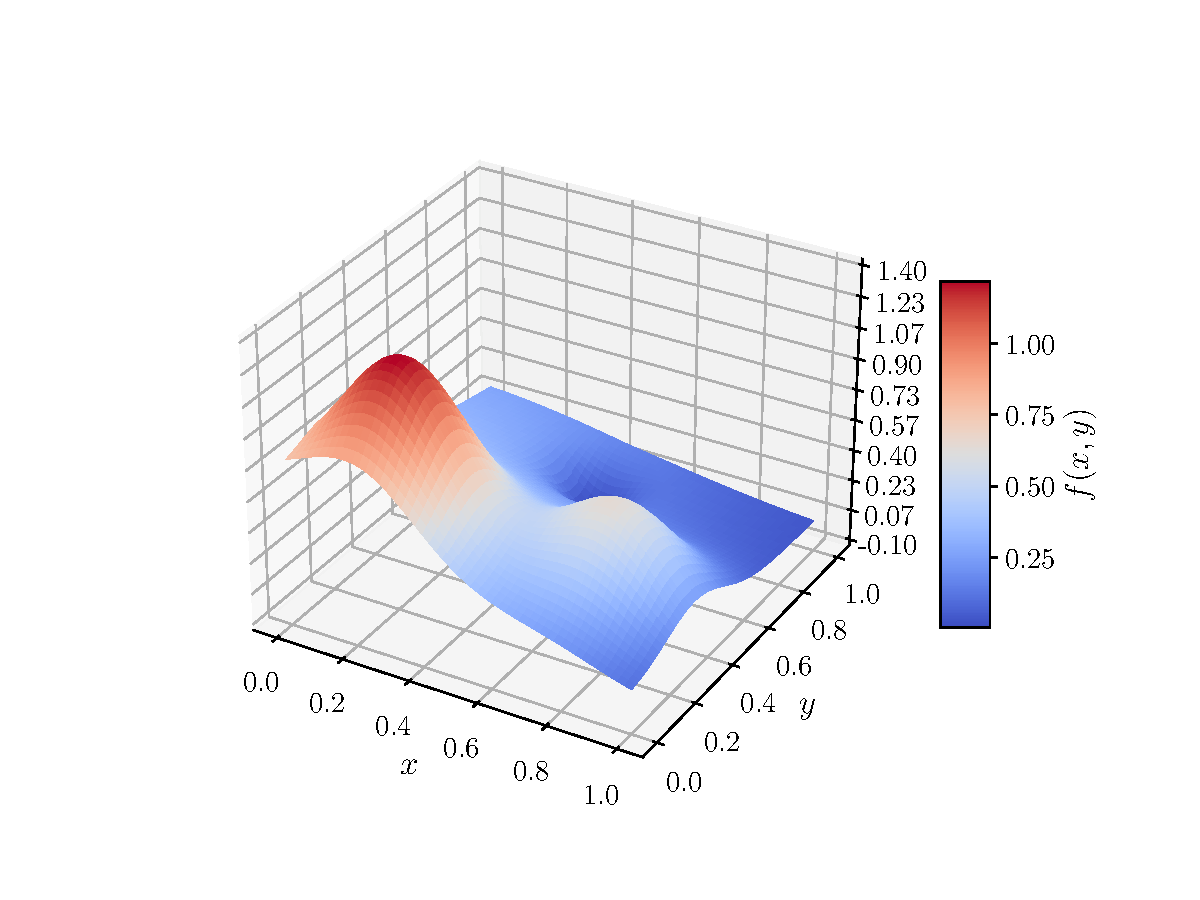
\includegraphics[trim=0 1.4cm 0 2cm,clip,width=\textwidth,keepaspectratio]{../figs/a_Franke_surf.pdf}
  \caption{Visualization of the two-dimensional Franke function expressed in \eqref{eq:Franke} on a $50\times50$ grid. In the right subplot we have added a noise contribution $\boldsymbol{\varepsilon}$ with standard deviation $\sigma=0.1$.}\label{fig:Franke}
  \vspace*{-5pt}
\end{figure*}


% EXPLAIN ANALYTICAL EXPRESSIONS ETC., REFER TO DERIVATIONS IN APPENDIX
% THESE ARE POSSIBLE SUBSECTIONS
\vspace*{-2.5pt}
\subsection{The Franke Function}\label{subsec:franke}
\vspace*{-2.5pt}
The Franke function is a two-dimensional synthetic function that is widely used in numerical analysis and computational mathematics, particularly in the fields of interpolation, regression analysis, and surface fitting. It is defined over the unit square $[0, 1] \times [0, 1]$ and expressed as
\begin{align*}
  f(x,y) =& \frac{3}{4} \exp{\left( -\frac{(9x - 2)^2}{4} - \frac{(9y - 2)^2}{4} \right)} \\
&+ \frac{3}{4} \exp{\left( -\frac{(9x + 1)^2}{49} - \frac{9y + 1}{10} \right)} \\
&+ \frac{1}{2} \exp{\left( -\frac{(9x - 7)^2}{4} - \frac{(9y - 3)^2}{4} \right)} \\
&- \frac{1}{5} \exp{\left( -(9x - 4)^2 - (9y - 7)^2 \right)}, \numberthis\label{eq:Franke}
\end{align*}
We will use the function multiple times throughout this work, as it produces a surface with both smooth and non-smooth regions, making it an excellent benchmark for testing regression and resampling algorithms. It simulates real-world data that may contain both complex variations and noise, mimicking scenarios that we will encounter as we move on to implementing the algorithms on actual simulation data.


\section{Methods \& Implementation}\label{sec:methods}
\subsection{Generating the Data}
\subsubsection{Synthetic Data}
The Franke function generated data used in this study was created by sampling the function on a grid of $N\times N$ points, where $N=50$. Furthermore, to emulate inherent variability and uncertainty in real-world data we added a gaussian noise component with a zero mean and standard deviation of $\sigma = 0.1$. The noise was added to simulate the inherent variability and uncertainty in real-world data. Visualizations of the function with and without added noise are plotted as surfaces in fig. \ref{fig:Franke}.

\subsubsection{Cosmological Simulation Data}
After implementing regression analysis and resampling methods using the Franke function we repeated the process using data from an N-body simulation of dark matter structure formation made with the public G\begin{footnotesize}ASOLINE\end{footnotesize}2 SPH code \cite{gasoline}. The initial conditions for the simulation were generated with MUSIC (MUlti-Scale Initial Conditions) \cite{music}, and standard Planck cosmology parameters $\Omega_\text{m}=0.3077$, $\Omega_{\Lambda}=0.6923$ and $H_0=67.81\:\text{km/s/Mpc}$ were used. The simulation box has length, width and height $L=20\:\text{Mpc}$, corresponding to a $500\times500\times500$ grid, and contains $64^3$ dark matter particles. 

The output data includes 128 ``snapshots'' of the box through time, where the time paramater in the simulation is the scale factor, defined as
\begin{equation*}
  a = \frac{1}{1+z}.
\end{equation*}
Here $z$ is the cosmological redshift, which is 0 today and thus in the 128th snapshot. We focused on the dark matter density $\rho$, and studied a snapshot at redshift $z\approx12.88$ because the distribution of $\rho$ is smoother at larger $z$. To get a function of two variables we averaged over one of the three axes so that we get a 2D grid, and because the density is so large and vastly different at different points in the box we took $\ln\rho$ to be our dependent variable instead of $\rho$. The resulting data is visualized as a contour plot and a surface plot in figure \ref{fig:density}. We chose not to add a synthetic noise component to this data, i.e. $\sigma=0$ in this case, since the simulation output can be interpreted as the true data if we were to perform real observations of dark matter density.

\begin{figure*}
  \vspace*{-5pt}
  \centering %Centers the figure
  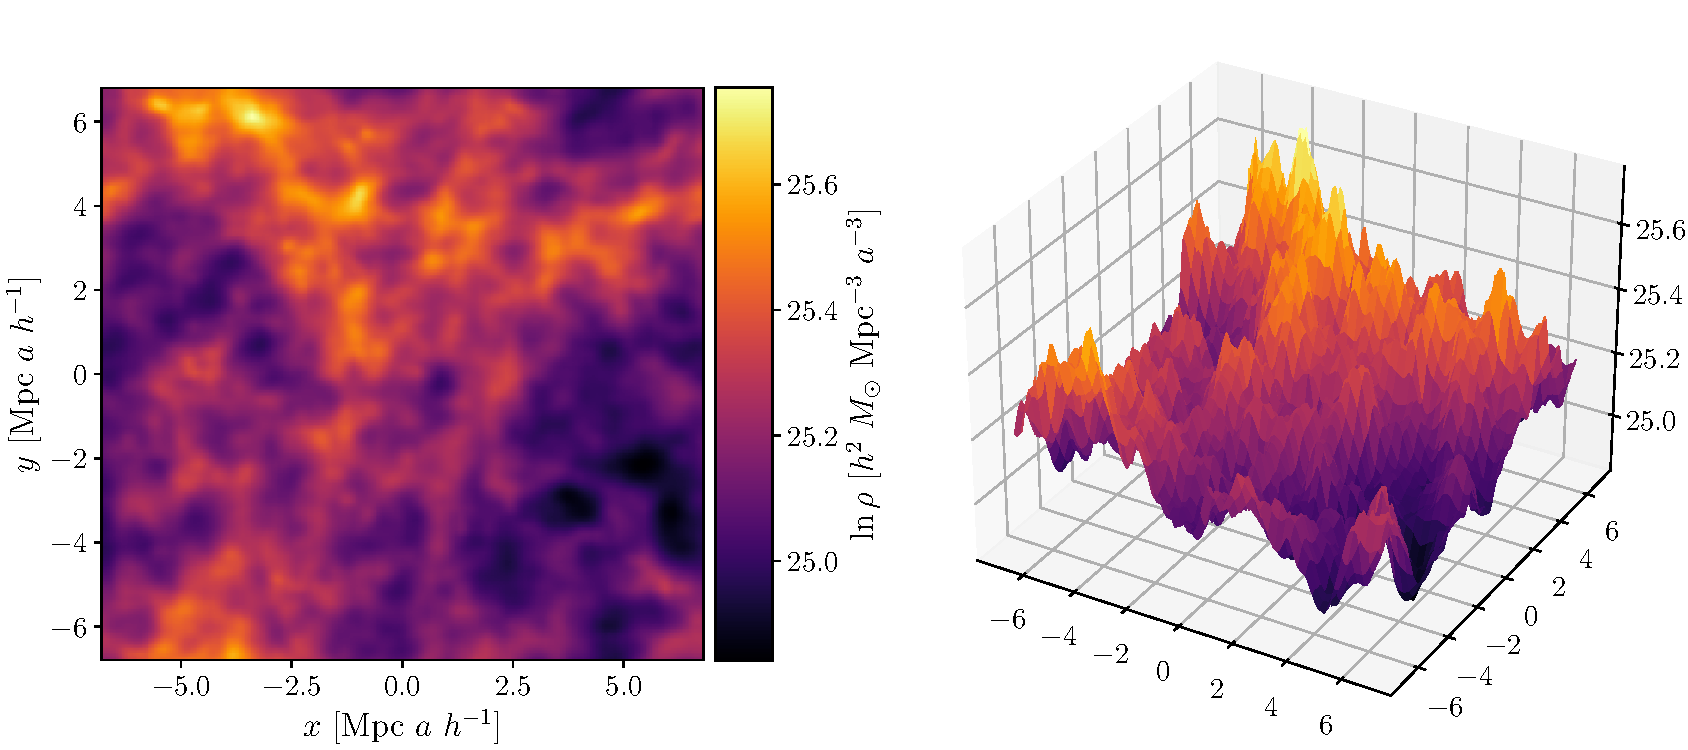
\includegraphics[width=0.9\textwidth]{../figs/density.pdf}
  \caption{Logarithm of dark matter density in the simulation box averaged over one of the three axes at redshift $z\approx12.88$. Visualized as contour plot on the left and as surface plot on the right. Because the Universe expands as time goes on the box does as well, and we therefore scale the coordinates of the box by multiplying with $a$. Similarly, space between the dark matter particles also increases with time, which is why the density is scaled by multiplying with $a^{-3}$. G\begin{footnotesize}ASOLINE\end{footnotesize}2 uses the rest of the scaling factors by default.}\label{fig:density}
  \vspace*{-5pt}
\end{figure*}



\subsection{Regression Analysis}
\subsubsection{Creating the Design Matrix}
Our first step when performing regression analyses on our data was to extend the design matrix $\mathbf{X}$ to the situation when we have two independent variables $\mathbf{x}$ and $\mathbf{y}$ instead of one $\mathbf{x}$. We then use $\mathbf{z}$ to denote our dependent variable. In the case of polynomial regression of degree $p$ with one independent variable vector $\mathbf{x}=\begin{pmatrix} x_0 &\ldots&x_{n}\end{pmatrix}^\top$ the design matrix has the form
\begin{equation*}
  \mathbf{X} = \begin{bmatrix}
    1 & x_0 & x_0^2 & \ldots & x_0^p
    \\
    1 & x_1 & x_1^2 & \ldots & x_1^p
    \\
    \vdots&\vdots&\vdots&\ddots&\vdots&
    \\
    1 & x_{n} & x_{n}^2 & \ldots&x_{n}^p
  \end{bmatrix}.
\end{equation*}
The feature vector in this case is $\boldsymbol{\beta}=\begin{pmatrix} \beta_0 &\ldots&\beta_{p}\end{pmatrix}^\top$, hence it is a column vector of length $p+1$, while our design matrix has dimensions $(n+1)\times (p+1)$

When we have two independent variables representing physical coordinates in a grid, each combination of $x_i$ and $y_j$ corresponds to a unique component $z_{ij}$ in $\mathbf{z}$. If $\mathbf{x}$ and $\mathbf{y}$ contain $n_x+1$ and $n_y+1$ components, respectively, the design matrix for polynomial degree $p$ then becomes
\begin{equation*}
  \mathbf{X} \hspace{-2pt}=\hspace{-3pt}\begin{bmatrix}
    1 & x_0 & y_0 & \ldots&x_0^p & x_0^{p-1}y_0 &\ldots& x_0y_0^{p-1}&y_0^p
    \\
    1 & x_1 & y_0 & \ldots & x_1^p & x_1^{p-1}y_0 &\ldots& x_1y_0^{p-1}&y_0^p
    \\
    \vdots&\vdots&\vdots&\ddots&\vdots&\vdots&\ddots&\vdots&\vdots
    \\
    1 & x_{n_x} & y_{0} & \ldots&x_{n_x}^p & x_{n_x}^{p-1}y_0 &\ldots& x_{n_x}y_0^{p-1}&y_0^p
    \\
    1 & x_0 & y_1 & \ldots& x_0^p & x_0^{p-1}y_1 &\ldots& x_0y_1^{p-1}&y_1^p
    \\
    \vdots&\vdots&\vdots&\ddots&\vdots&\vdots&\ddots&\vdots&\vdots
    \\
    1 & x_{n_x} & y_{n_y} & \ldots& x_{n_x}^p & x_{n_x}^{p-1}y_{n_y} &\ldots& x_{n_x}y_{n_y}^{p-1}&y_{n_y}^p
  \end{bmatrix}.
\end{equation*}
We thus see that for polynomial degree 0 we have one column, three columns for first degree, six for second, ten for third, etc. This is a well known series of numbers, and we can express the number of features $l$ in terms of the polynomial degree $p$ as
\begin{equation*}
  l = \frac{1}{2}(p+1)(p+2).
\end{equation*}
Our design matrix thus has dimensions $N\times l$ where $N=(n_x+1)\times(n_y+1)$.


\subsubsection{Preprocessing}
As a first step in our analyses it was essential to employ data scaling in order to ensure numerical stability. By utilizing the \verb|StandardScaler| function from the scikit-learn library \cite{scikit-learn} we standardized our datasets by subtracting the mean and dividing by the standard deviation for each feature. Although the data generated by the Franke function and the cosmological simulation data used in subsequent analyses are inherently two-dimensional and may not exhibit significant variation in scale between features, scaling still provides consistent benefits.

The primary motivation for applying this scaling function was to enhance the performance and stability of our algorithms. Scaling prevents features with larger magnitudes from disproportionately influencing the objective function and helps balance minor discrepancies between features that might affect the learning process. The performance of regression models is generally significantly improved when the data is scaled, as it ensures faster convergence and reducing the risk of numerical instability.

Another important preprocessing step was splitting the data into training and test sets, which enables the evaluation of the model's performance on unseen data and helps in assessing its generalization capabilities. We used the \verb|train_test_split| function from the scikit-learn library with a test size of 0.2. This ensured that a random 20\% of the data was reserved for testing, while the remaining 80\% was used to train the model. By splitting the data in this manner we could evaluate the model's performance on ``new'' data and determine how well it generalized to unseen samples.

To illustrate the impact of scaling, we computed the $\beta$-coefficients using unscaled (or ``raw'') and scaled versions of our design matrices when training OLS models on the Franke function-generated data as well as on the cosmological simulation data. We tested polynomial degrees in the intervals $[1,6]$ and $[1,41]$ (skipping every other degree) for the Franke and dark matter data, respectively. Visualizing the resulting coefficients allowed us to observe how scaling influenced the coefficients and affected the models' performances. 

\subsubsection{Exploring Complexity Dependency Using OLS}
Investigating the dependency on polynomial degree was a critical aspect of understanding how the regression models performed under varying conditions. By increasing the polynomial order, we enhanced our model's capacity to fit more complex patterns in the data. However, this also raised the risk of overfitting, where the model might capture noise along with the underlying structure. To explore this, we evaluated the performance of the models across different polynomial degrees using metrics such as the MSE and $R^2$ scores mentioned in the previous section. These evaluations allowed us to quantify how well each model balanced bias and variance. 

Using OLS we systematically varied the polynomial degree from 1 to 6 when fitting to the Franke function-generated data. For the cosmological simulation data we followed a similar approach, but because of the heightened complexity of this data we varied the polynomial degrees from 1 up to and including 41, using only every other step. The models' performances were then evaluated on the test portions of the datasets using the MSE and $R^2$ metrics. To visually assess the models' fit to the cosmological data and identify any potential overfitting or underfitting issues we also contour plotted and analyzed the fits for polynomial degrees 5, 10, 20, 30, and 50. Additionally, we produced a 3D surface of the 30-degree polynomial fit and plotted this alongside the raw data to help visualize the model's performance in capturing the underlying patterns.

\subsubsection{Introducing Regularization}
To further explore complexity dependency we introduced regularization terms through both Ridge and Lasso regression. In both cases we tested polynomial degrees ranging from 1 to 41 when training our models on the Franke function-generated data, using every second degree for Ridge and every fourth for Lasso, to see if we would observe any signs of overfitting. When moving on to the cosmological simulation data we used 11 evenly spaced polynomial degrees $\in[1,31]$ instead. This restricted choice of degrees was motivated by the runtime constraints of the algorithms, as this was a much more prominent issue due to the increased size of the dataset.

To thoroughly evaluate the models, we systematically tested a range of values for the hyperparameter $\lambda$, from $10^{-5}$ to 1. For the Franke data we used 30 values in this range, evenly spaced on a logarithmic scale, whereas only 11 values were tested for the cosmological simulation data due to the runtime constraint. Each of the $\lambda$ values were combined with every polynomial degree within the aforementioned ranges. The resulting MSE and $R^2$ scores were computed and contour plotted as functions of both $\lambda$ and polynomial degree. This dual-parameter visualization allowed us to identify the optimal combination of polynomial degree and $\lambda$ for each model, thereby providing a comprehensive view of how model performance changes with varying complexity and regularization strength.


\subsection{Bias-Variance Tradeoff}
As a starting point in our study of the bias-variance tradeoff explained in \cref{subsec:tradeoff}, and to validate our implementations, we attempted to imitate the analysis illustrated in fig. 2.11 in Hastie et al. \cite{ESL}, which we have included in \cref{fig:Hastie}. Specifically, we implemented OLS regression on the Franke function-generated data for polynomial degrees $\in[1,81]$ in steps of 4, and computed the MSE evaluated on both the training and test portions for each degree. The generation and splitting of the Franke data were conducted as described previously. 

\begin{figure}
  \centering %Centers the figure
  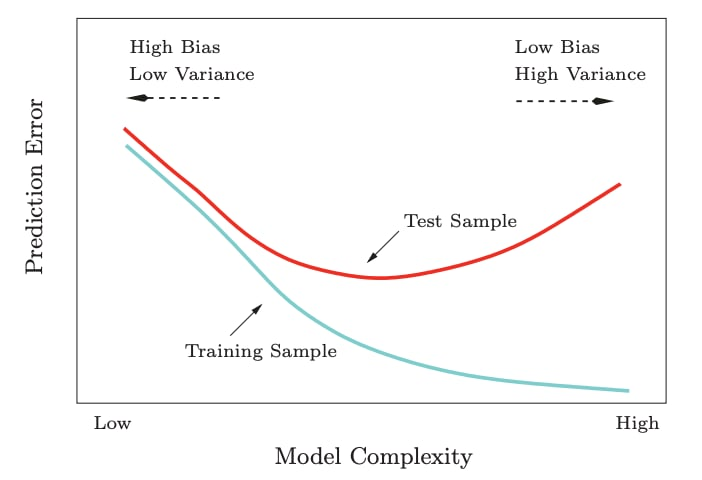
\includegraphics[width=\columnwidth]{../figs/hastie_bias_variance_tradeoff.jpg}
  \caption{Illustration of bias-variance trade-off as a function of model complexity, taken from fig. 2.11 in Hastie, Tibshirani, and Friedman \cite{ESL}}\label{fig:Hastie}
\end{figure}

\subsubsection{Bootstrap With OLS}
To further explore the bias-variance tradeoff and study the effects of resampling we implemented the bootstrap technique, which involved resampling the training data multiple times and fitting an OLS model to each resampled dataset. This was accomplished using the \verb|resample| function from the scikit-learn library. To evaluate the model's performance we averaged over the MSE, bias and variance values computed for each resampled dataset.

For the Franke function-generated data we designed four different cases, each varying a specific parameter to separately investigate the influence of model complexity, the number of data points, bootstrap steps, and test size fraction. The default values we used were polynomial degree 5, 50 data points (i.e. a $50\times50$ grid), 100 bootstraps, and a test size of 20\%. When varying the parameters in each respective scenario we used the following: 
\begin{itemize}
   \item [-] Polynomial degree: from 1 to 41 with a step of 2
   \item [-] Number of data points: [10, 20, 30, 40, 50, 100, 150, 200, 300, 400, 500, 1000]
   \item [-] Number of bootstraps: [1, 2, 5, 10, 20, 50, 100, 200, 500, 1000, 2000, 5000, 10000]
   \item [-] Test size: ranging from 5\% of the entire set to 95\% with a step of 5\%
\end{itemize}
For each case we computed the model's MSE, bias and variance and plotted them against the varying parameter to analyze how its performance changed with different settings. We did not repeat this process using the cosmological simulation data. This was mostly to save time, but also because this part of the analysis involved varying so many parameters that we believed repeating the process on a different set would contribute minimally to our discussions of the bias-variance tradeoff.

\subsection{Cross-Validation}
After implementing the bootstrap resampling technique we moved on to $k$-fold cross-validation. For this part of the analysis we used the \verb|KFold| function from the scikit-learn library, which generates indices that facilitate the partitioning of a dataset into $k$ equally-sized folds. We employed the shuffle option to randomly shuffle the data before partitioning, which helps ensure that the data distribution is random and reduces potential biases stemming from the original order of the data. 

We implemented cross-validation for OLS, Ridge, and Lasso regression by passing the chosen model, the design matrix, and the target variable together with the indices generated by \verb|Kfold| to either \verb|cross_val_predict| or \verb|cross_val_score|, both of which are functions from the scikit-learn library. The former function call provided the predicted values from each partition averaged over the $k$ folds, which we used to evaluate the model's generalization. The latter function returned the negative MSE for each fold, so we averaged these across all folds and adjusted the sign to obtain the final cross-validated MSE for the model.

For the Franke function-generated data we conducted cross-validation with $k \in [5,15]$ for polynomial degrees $\in [1,15]$ and visualized the MSE's as function of both parameters in a contour plot. In order to compare this method with the bootstrap technique we also plotted the estimated MSE's obtained with 100 bootstraps for the same degrees. We repeated this process with the cosmological simulation data as well, this time using polynomial degrees $\in [1, 31]$ with a step of 3.

To study how cross-validation affects the qualities of the fits obtained using Ridge and Lasso regression we repeated the aforementioned process with the same polynomial degrees and $k$'s, once with $\lambda = 0.001$ and again with $\lambda = 0.5$, but excluding bootstrap this time. Lastly, we used \verb|cross_val_predict| to estimate fits to the cosmological simulation data using OLS, Ridge and Lasso with polynomial degree 30, $k = 5$, and $\lambda = 0.001$ for the latter two. We then contour plotted the fits together with the actual data in order to visually assess the models' performances and the effect of cross-validation, and to properly compare the three regression variants.


\subsection{The Program}\label{subsec:program}
\subsubsection{Code Structure}\label{subsubsec:codestructure}
All the source code that we developed and used to produce our results is available on our GitHub repository, linked in \cref{appsec:code}. The \verb|README.md| file contains the entire project structure. Our code is divided into the following files and notebooks:

\verb|franke.ipynb|: Jupyter notebook containing the analysis of the Franke function data, which we used to to validate our implementation.

\verb|data_analysis.ipynb|: Jupyter notebook containing the analysis of the dark matter density data. Here we have applied and further tested our regression models.

\verb|functions.py|: Python script containing all the functions used in the notebooks, all properly documented. The file includes a main block, testing the functions.


\subsubsection{Tools}\label{subsubsec:tools}
All our code is written in Python \cite{Python}, and we used scikit-learn \cite{scikit-learn} to create most of our models. To vectorize our code we used \verb|numpy| \cite{Numpy}, and for visualization we used \verb|matplotlib.pyplot| \cite{Matplotlib}. Code completion and debugging was done in Visual Studio Code \cite{VSCode} with additional assistance of GitHub Copilot \cite{Copilot}. We used \verb|git| \cite{Git} for version control, and \verb|GitHub| \cite{GitHub} for remote storage of our code.


\section{Results \& Discussion}\label{sec:results discussion}
\subsection{Effects of Data Scaling}\label{subsec:scaling effect}
In the upper part of \cref{fig:error scaled vs raw} we have plotted the estimated MSE and $R^2$ scores evaluated on the Franke function test for polynomial degrees $\in[1,6]$. The left and right columns show the scores computed for the raw and scaled data, respectively. As expected there looks to be a constant factor between the raw and scaled MSE's, while the $R^2$ scores are equal in both cases. This is because $y_i$, $\tilde{y}_i$ and $\overline{y}$ (or in our case, $z_i$, $\tilde{z}_i$ and $\overline{z}$) are scaled equally, and from eq. \eqref{eq:R2} we thus see that the scaling cancels out from the numerator and denominator in the second term. 

\begin{figure*}
  \vspace*{-5pt}
  \centering %Centers the figure
  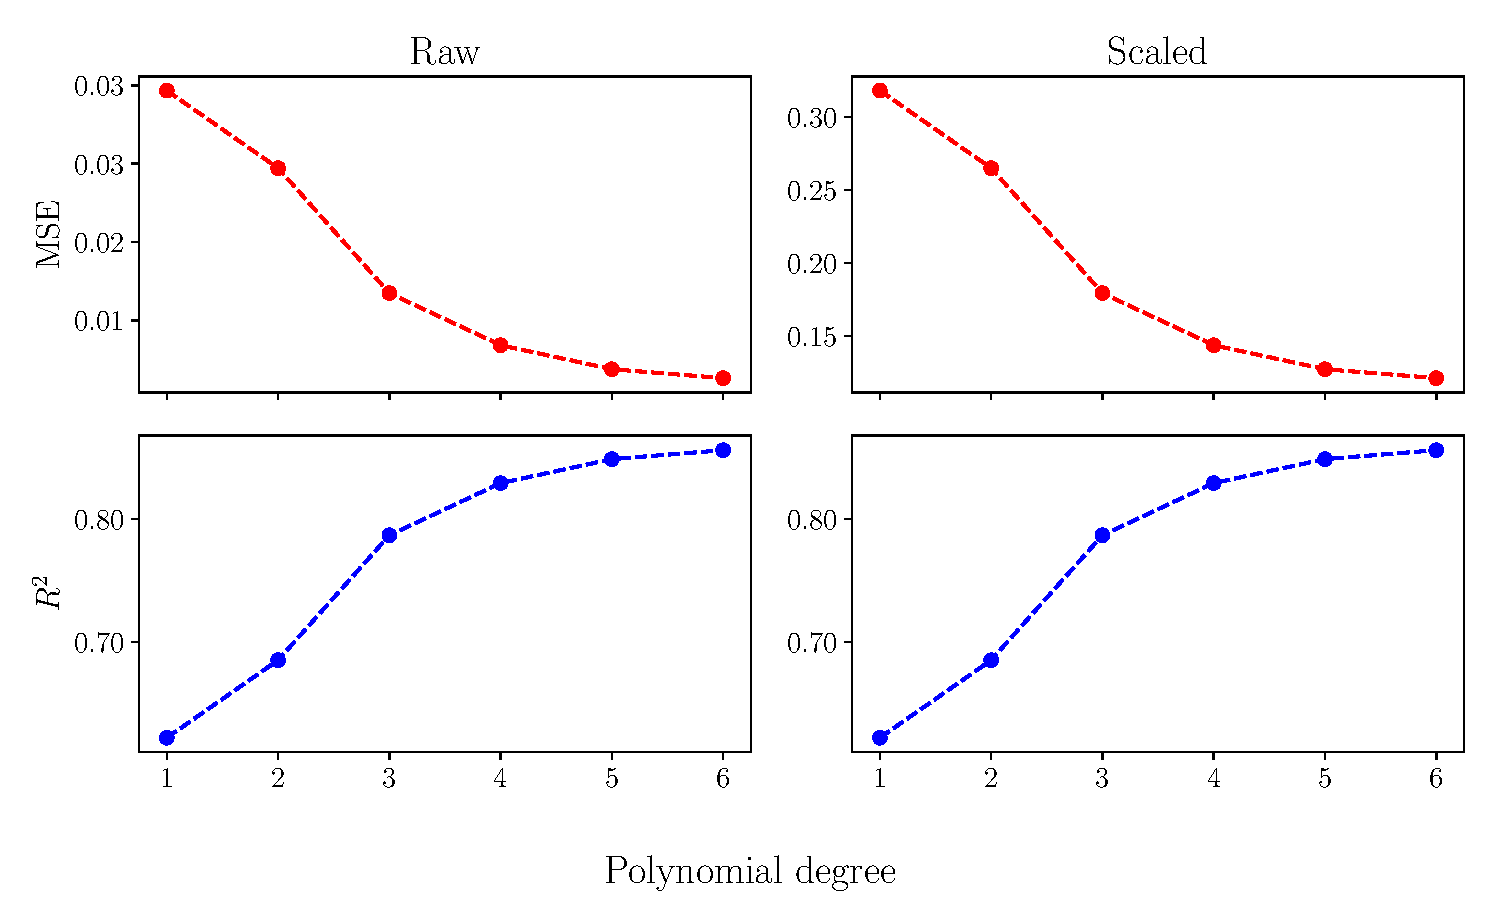
\includegraphics[trim = 0 1.5cm 0 0,clip,width=0.75\textwidth,keepaspectratio]{../figs/a_error_scaled_vs_raw.pdf}
  \centering
  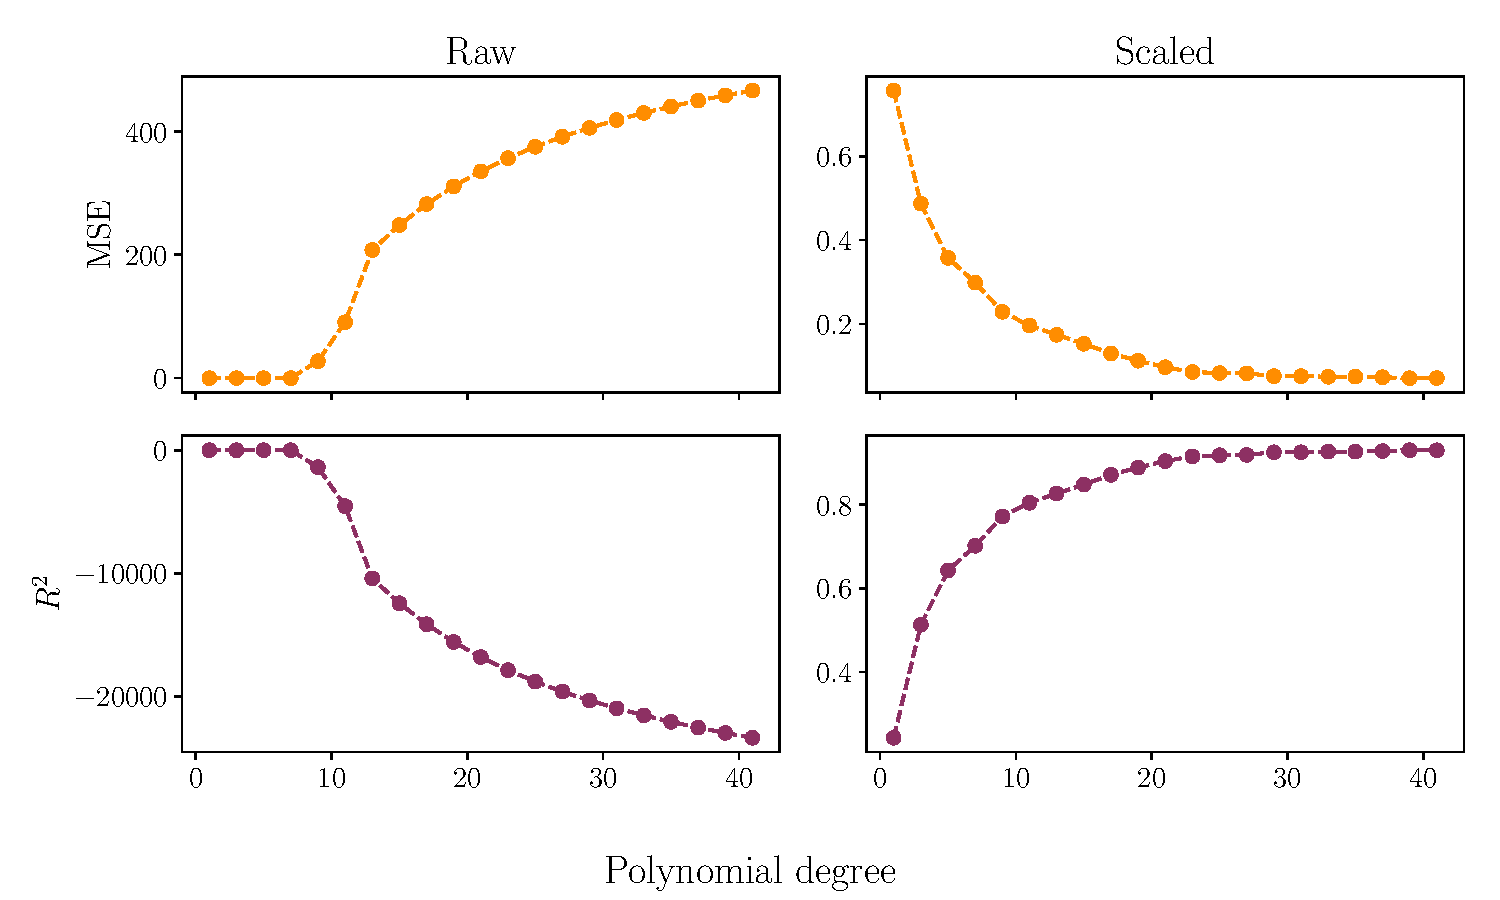
\includegraphics[width=0.75\textwidth]{../figs/g_error_scaled_vs_raw.pdf}
  \caption{MSE (upper rows) and $R^2$ (lower rows) evaluated on the Franke function test set (upper section) and the cosmological simulation test set (lower section) using unscaled (left column) and scaled (right column) values. For the Franke function we have used polynomial degrees in the interval $[1,6]$, while for the cosmological data we have used every other degree in the interval $[1,41]$.}\label{fig:error scaled vs raw}
  \vspace*{-5pt}
\end{figure*}

One might expect to see the same effects of scaling for the cosmological simulation data, but in the lower part of \cref{fig:error scaled vs raw} we see that this is not the case. Here we have plotted the MSE and $R^2$ scores for 21 evenly spaced polynomial degrees in the interval $[1,41]$, and we see that for degrees $\gtrsim9$ the raw scores diverge from the expected trend. Instead of a decreasing MSE and increasing $R^2$ as in the scaled case we get MSE's over 400 and very large, negative $R^2$ scores, a metric that should never be negative in the first place. This clearly shows why it is beneficial to scale the data, since it is safe to assume that the raw data catastrophe occurs due to numerical instability caused by loss of floating point precision. Moreover, we see that we never reach a turning point in the scores where they start to worsen with polynomial degree, which makes sense considering the complexity of our dataset.

In fact, we see from the bottom part of \cref{fig:beta scaled vs raw} that the scaled coefficients for the fits to the cosmological data (plotted in orange) grow in orders of magnitude with complexity (cirka up until degree $21$, where the largest stay around $10^4$), while the raw coefficients (plotted in purple) fall to zero around polynomial degree 9. The reason for the strong increase in the $\beta_\text{scaled}$'s is that $\mathbf{x}$ and $\mathbf{y}$ (both raw and scaled) are centered at 0, and in the scaled case these are divided by their standard deviations, hence most of the highest order polynomial terms decrease with the degree. We thus need very large coefficients for their contributions to the fit to be noticeable. The $\beta_\text{raw}$'s must be much smaller since the highest order terms grow rapidly with degree at the edges of the box, and eventually we encounter floating point errors. This is contrary to the coefficients estimated for the Franke function, where generally $\beta_\text{raw}\geq\beta_\text{scaled}$, as seen in the top part of the figure. This is because the Franke function is defined over the unit square, hence the raw coefficients grow with polynomial degree as well.

\begin{figure}
  \vspace*{-5pt}
  \centering %Centers the figure
  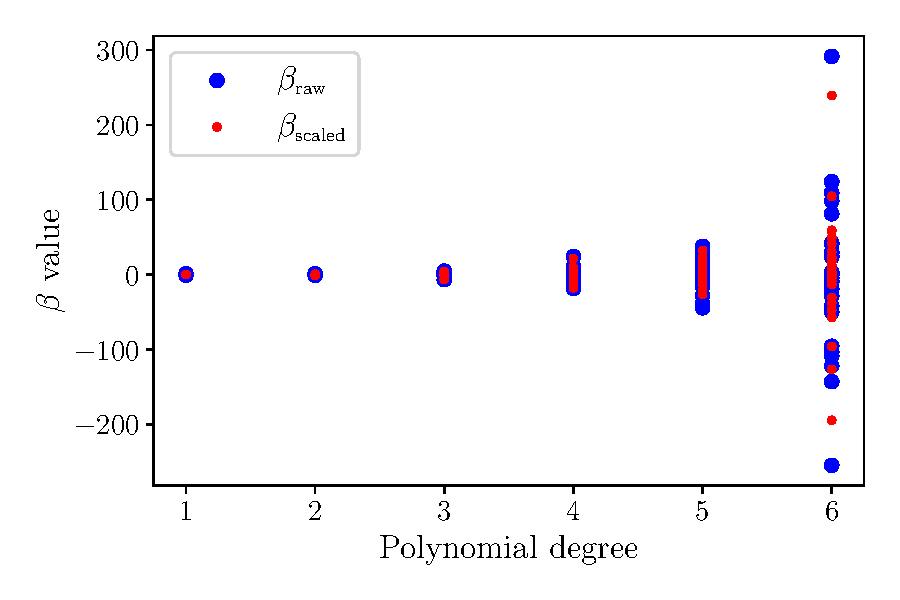
\includegraphics[trim = 0 1.3cm 0 0,clip,width=\columnwidth,keepaspectratio]{../figs/a_beta_scaled_vs_raw.pdf}
  \centering %Centers the figure
  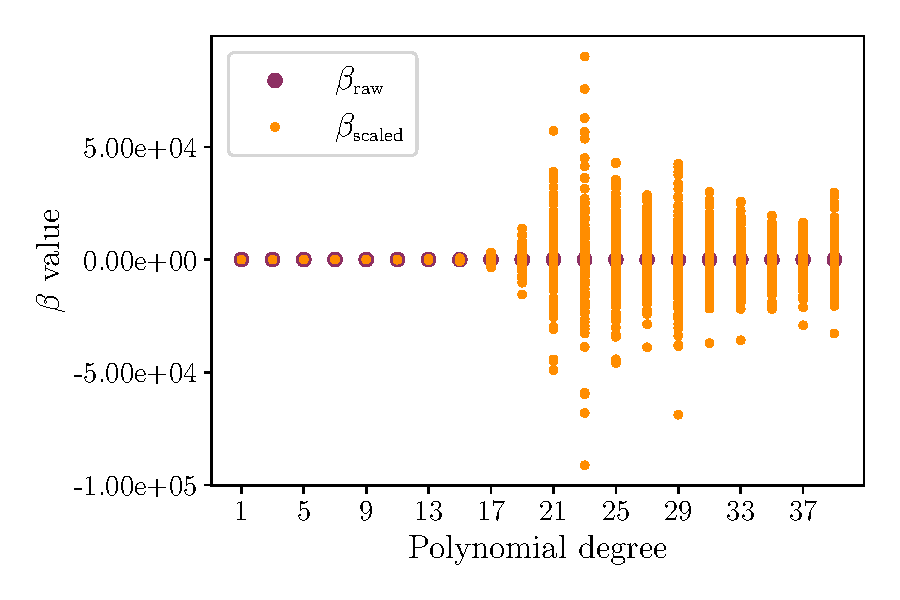
\includegraphics[width=\columnwidth]{../figs/g_beta_scaled_vs_raw.pdf}
  \caption{The coefficients $\beta$ for the Franke (top) and cosmological (bottom) fits estimated using unscaled and scaled data, plotted for polynomial degrees in the intervals $[1,6]$ and $[1,41]$ for Franke and dark matter, respectively. We have used a logarithmic scale for the $\beta$'s in the latter case.}\label{fig:beta scaled vs raw}
  \vspace*{-5pt}
\end{figure}

\subsection{Hyperparameter Dependency}\label{subsec:hyperparameter}
% \subsubsection{Ridge}
In \cref{fig:MSE R2} we have contour plotted MSE and $R^2$ scores evaluated on the test portion of the Franke function data for Ridge (top section) and Lasso (bottom section) regression. Here we see that in both cases it is generally favorable to opt for smaller hyperparameters, although Lasso is much more sensitive to changes in $\lambda$ above a threshold of around 7 than what Ridge is. This is because Lasso regression employs the $L^1$ norm, which means that the coefficients can be driven completely to zero if the hyperparameter is large enough, contrary to the $L^2$ norm used in Ridge egression. Thus, as we continue increasing the value of $\lambda$ in Lasso above a certain value our fits will practically be zero at all points, and the scores will then stay constant.

\begin{figure*}
  \vspace*{-5pt}
  \centering %Centers the figure
  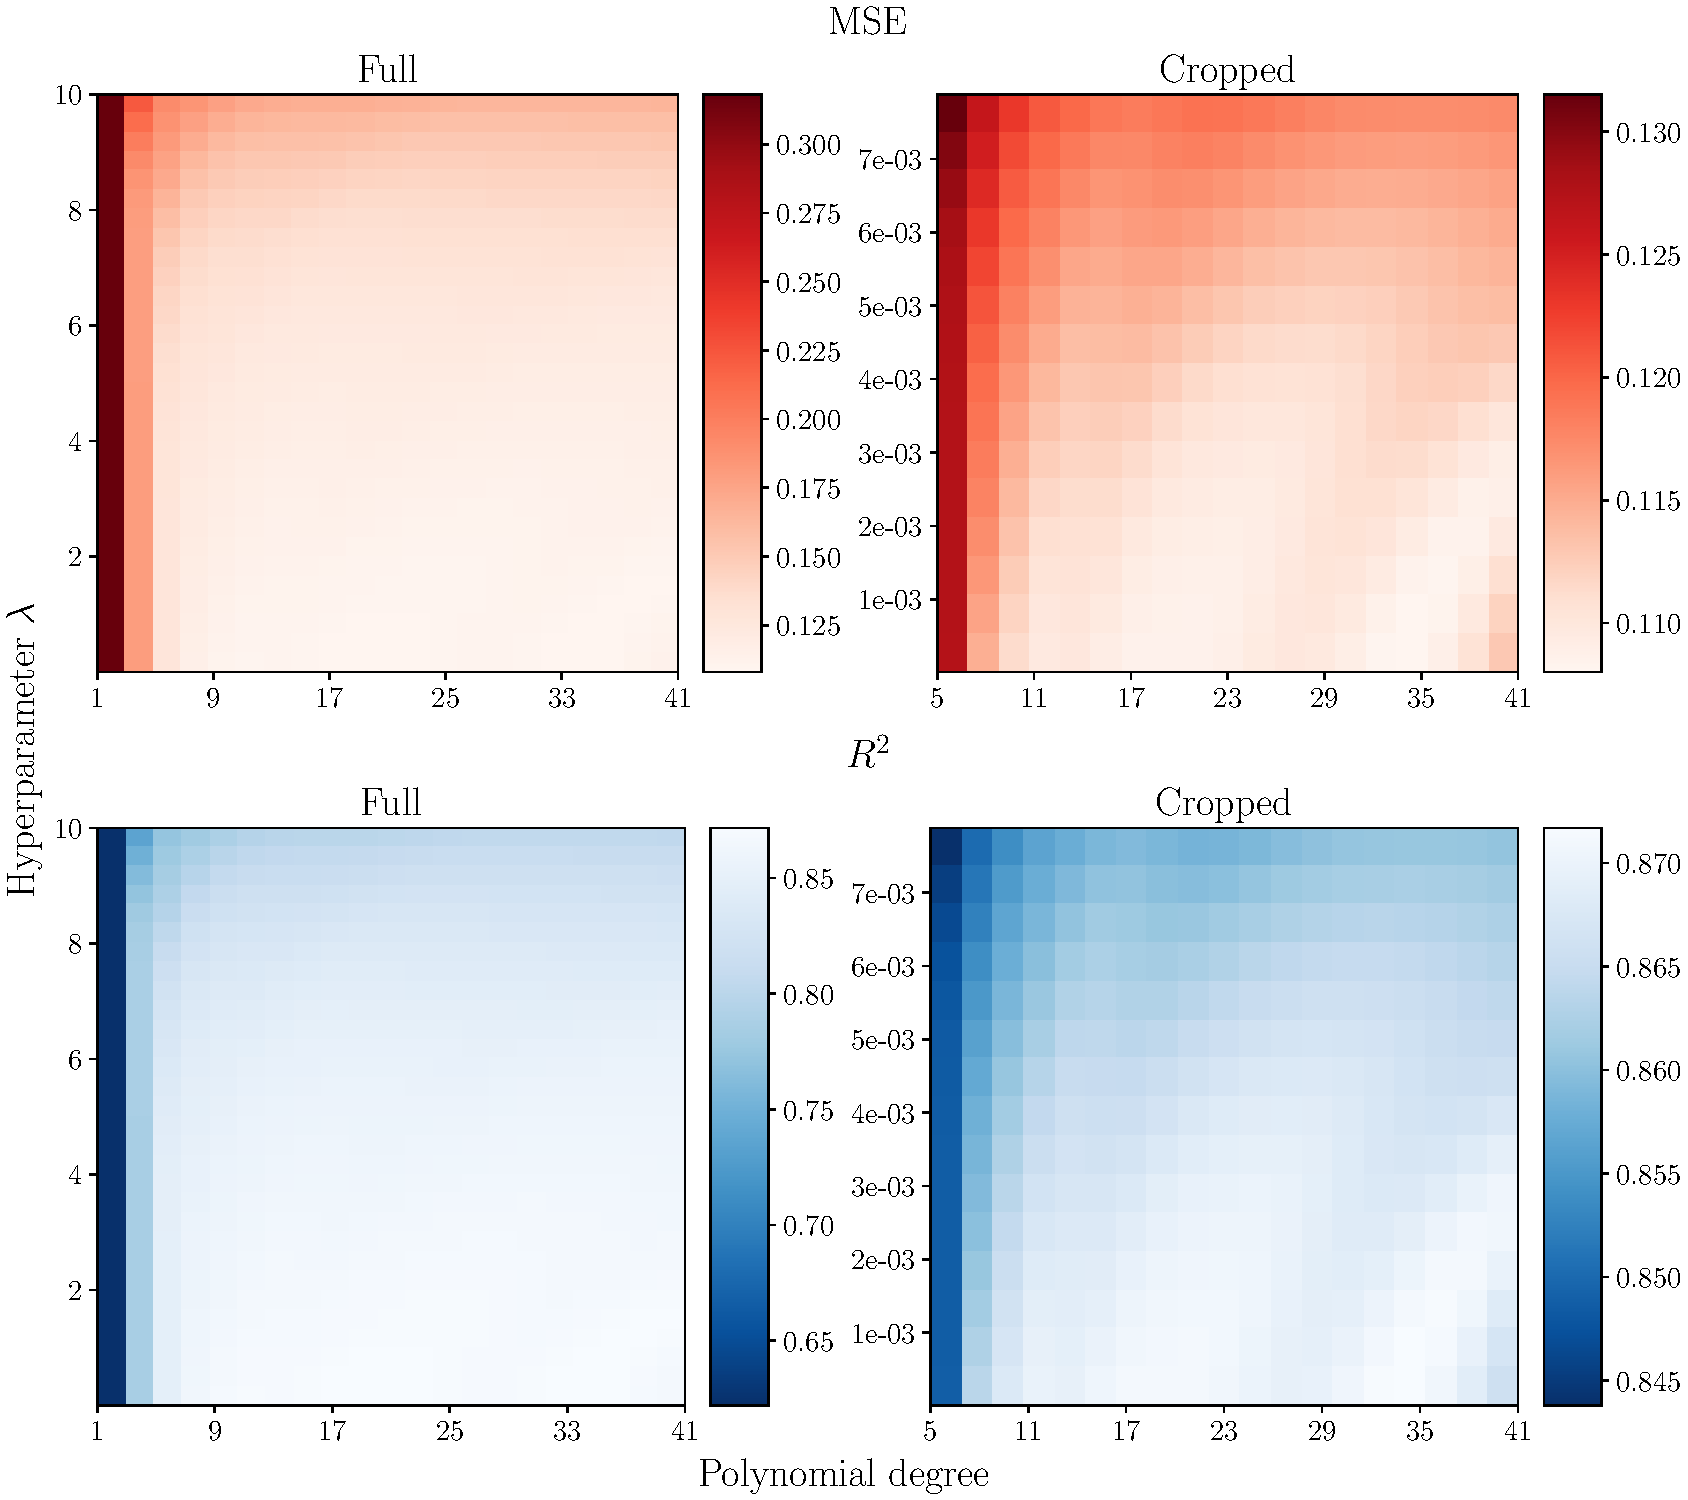
\includegraphics[width=0.7\textwidth]{../figs/b_MSE_R2.pdf}
  \centering
  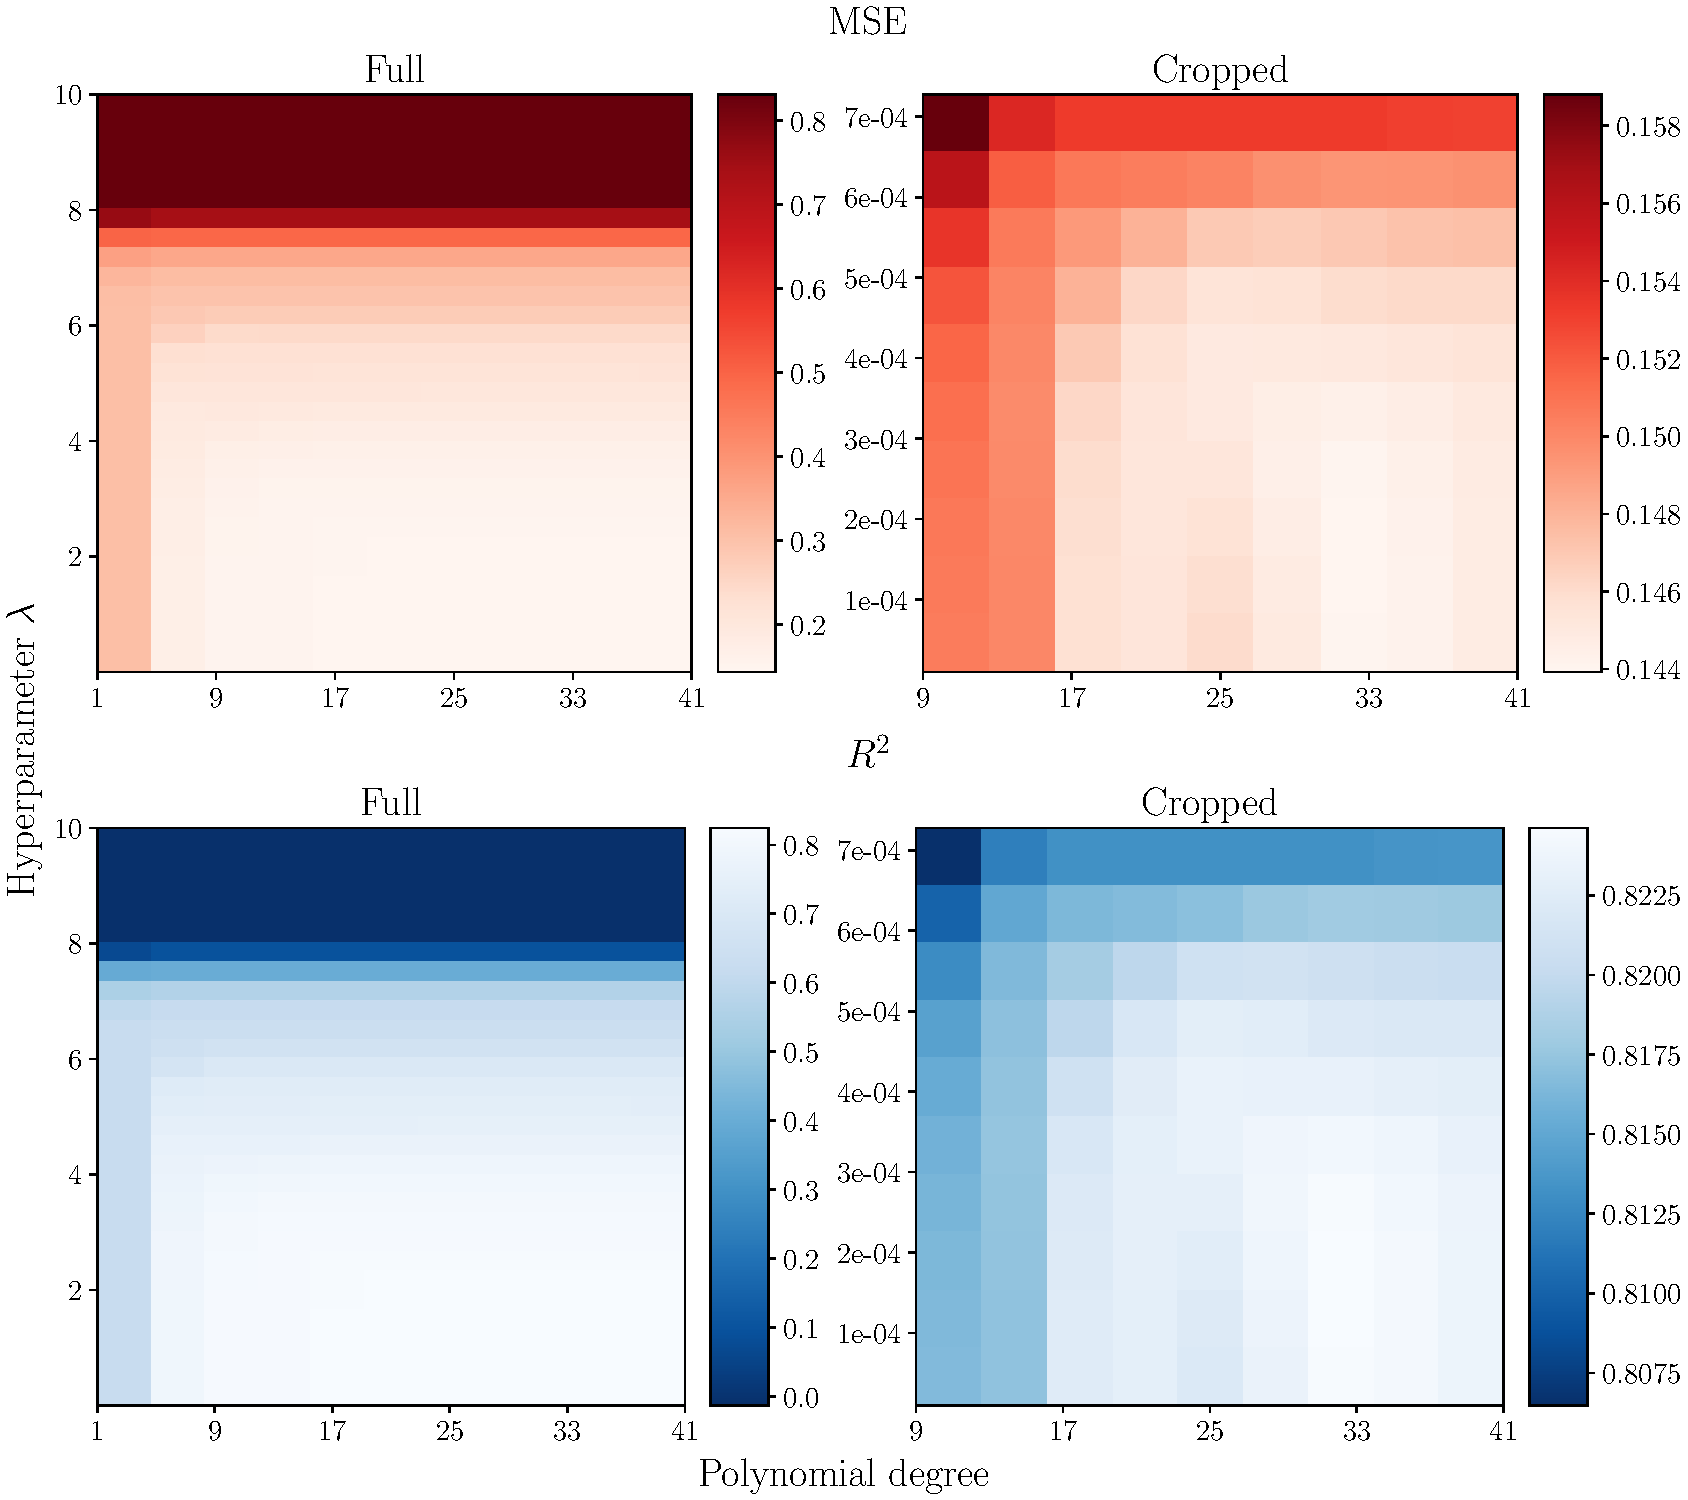
\includegraphics[width=0.7\textwidth]{../figs/c_MSE_R2.pdf}
  \caption{MSE (upper rows) and $R^2$ (lower rows) for Ridge (top section) and Lasso (bottom section) regression evaluated on the Franke test data. The scores vary with polynomial degree horizontally and hyperparameter $\lambda$ vertically. In the right columns we have cropped away degrees 1 and 3 (1 and 5) and the 15 (20) largest $\lambda$ values for Ridge (Lasso), purely for visualization purposes.}\label{fig:MSE R2}
  \vspace*{-5pt}
\end{figure*}

For Ridge we see that the increased error associated with a large $\lambda$ is smaller as we move to the highest complexities, which makes sense considering that we already had a good fit (low MSE and high $R^2$) for polynomial degrees around 5-6, hence the higher order terms are not as necessary. Since the $L^2$ norm ensures that the coefficients are shrinked uniformly, a large hyperparameter will thus have more severe consequences for the quality of the lower complexity fits. Moreover, we found that the scores' overall trend of the dependencies on polynomial degree and hyperparameter were similar for the cosmological data, for both Ridge and Lasso regression, as can be seen in \cref{appfig:g MSE R2} in \cref{appsec:figures}. 

In the right columns of figs. \ref{fig:MSE R2} and \ref{appfig:g MSE R2} we have cropped out the smallest polynomial degrees and largest hyperparameters. Here we can see that the scores solely improve as we move towards larger degree and smaller $\lambda$ for the dark matter data, while for the Franke data some combinations of degree and $\lambda$ lead to slightly better scores than others. Although these variations seem to follow some sort of pattern, at least for Ridge, looking at the values on the colorbar axes we see that they are very small, and they might just be random. For future studies this would be worth looking into.


\subsection{Bias-Variance Tradeoff}
\subsubsection{Training and Test Errors}
In \cref{fig:e train test} we have plotted MSE scores evaluated on the training and test portions of the Franke data as functions of polynomial degrees up to 81. Although our curves are not as smooth as those in fig. 2.11 from Hastie et al., the overall trend is similar. The main difference is that the errors fall much faster with complexity for low degrees, and the test error is very close to the training error for a wide range of polynomial degrees before it abruptly increases as we reach $\sim75$, contrary to the more smooth ``U-shape'' we see in their figure. It is worth noting that theirs is an illustration, though, and we can not know how complex the data is assumed to be relative to the Franke function, nor what exactly is meant by a ``high'' model complexity. The former affects how large the error is for the lowest polynomial degrees, and the magnitude of the test error at high complexity depends on both. 

\begin{figure}[h!]
  \vspace*{-5pt}
  \centering %Centers the figure
  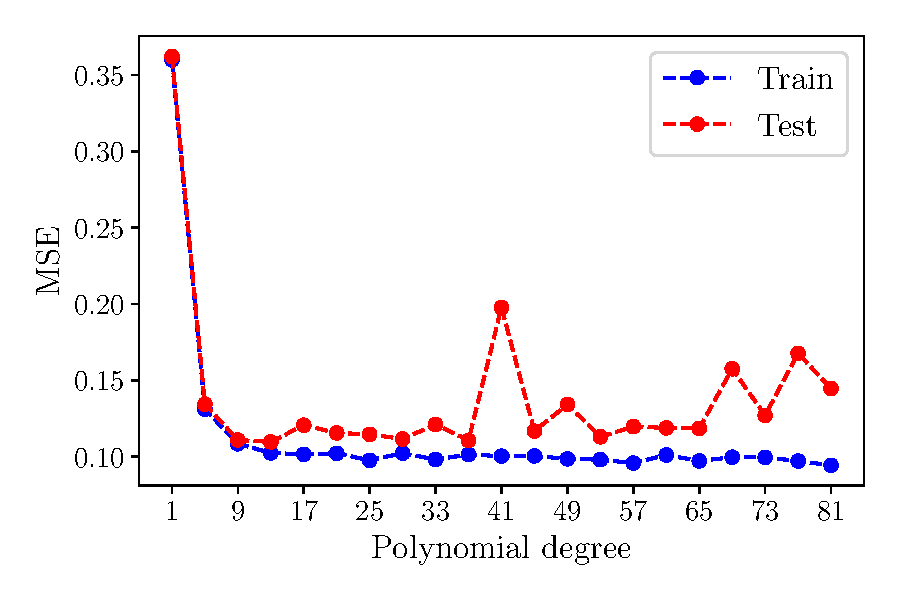
\includegraphics[width=\columnwidth]{../figs/e_MSE_train_test.pdf}
  \caption{MSE evaluated on the Franke function training set (blue) and test set (red) for 21 evenly spaced polynomial degrees in the interval $[1, 81]$.}\label{fig:e train test}
  \vspace*{-5pt}
\end{figure}

When studying the complexity and hyperparameter dependence of the Franke function MSE and $R^2$ scores, we saw that they continued to improve with complexity up to degree 41 and that vanishing $\lambda$ was the best option. We found this rather peculiar at first, as we would expect overfitting and thus a need for regularization at this level, considering the relatively low complexity of the Franke function and that the fits we obtained with polynomial degrees between 5 and 10 already seemed score-wise satisfactory. However, \cref{fig:e train test} offers an explanation to this result, since the test set MSE for OLS regression starts increasing well after we surpass polynomial degree 41. Also, Since we used $50\times50$ data points for the regression, the likelihood of fitting to random noise is smaller than if we had used, for example, $10\times10$ points. This is because, as the number of data points increases, the average of the true data plus noise approaches the sum of the true data's mean and the noise's mean. In our case, the noise has an expectation value of zero, so with more data points, the overall effect of noise on the model diminishes. 

\vspace*{-2.5pt}
\subsubsection{Parameter Dependencies of MSE, Bias and Variance}
In \cref{fig:e bias variance} we have plotted MSE, bias and variance for models trained using generated Franke data with bootstrapping as functions of polynomial degree, number of data points, number of bootstrap steps and test size fraction. Their dependencies on polynomial degree agree well with \eqref{eq:model error}, although we would expect the MSE to be slightly larger than the bias even when the model variance is $\sim0$, due to the contribution from the noise variance. We need to remember that the noise we added to our Franke data was generated using a standard deviation $\sigma=0.1$, hence this contribution $\sigma^2=0.01$ to the error is negligible compared to the bias at the lowest complexities, which lies in the range $[0.1,0.3]$. 

\begin{figure*}
  \vspace*{-5pt}
  \centering %Centers the figure
  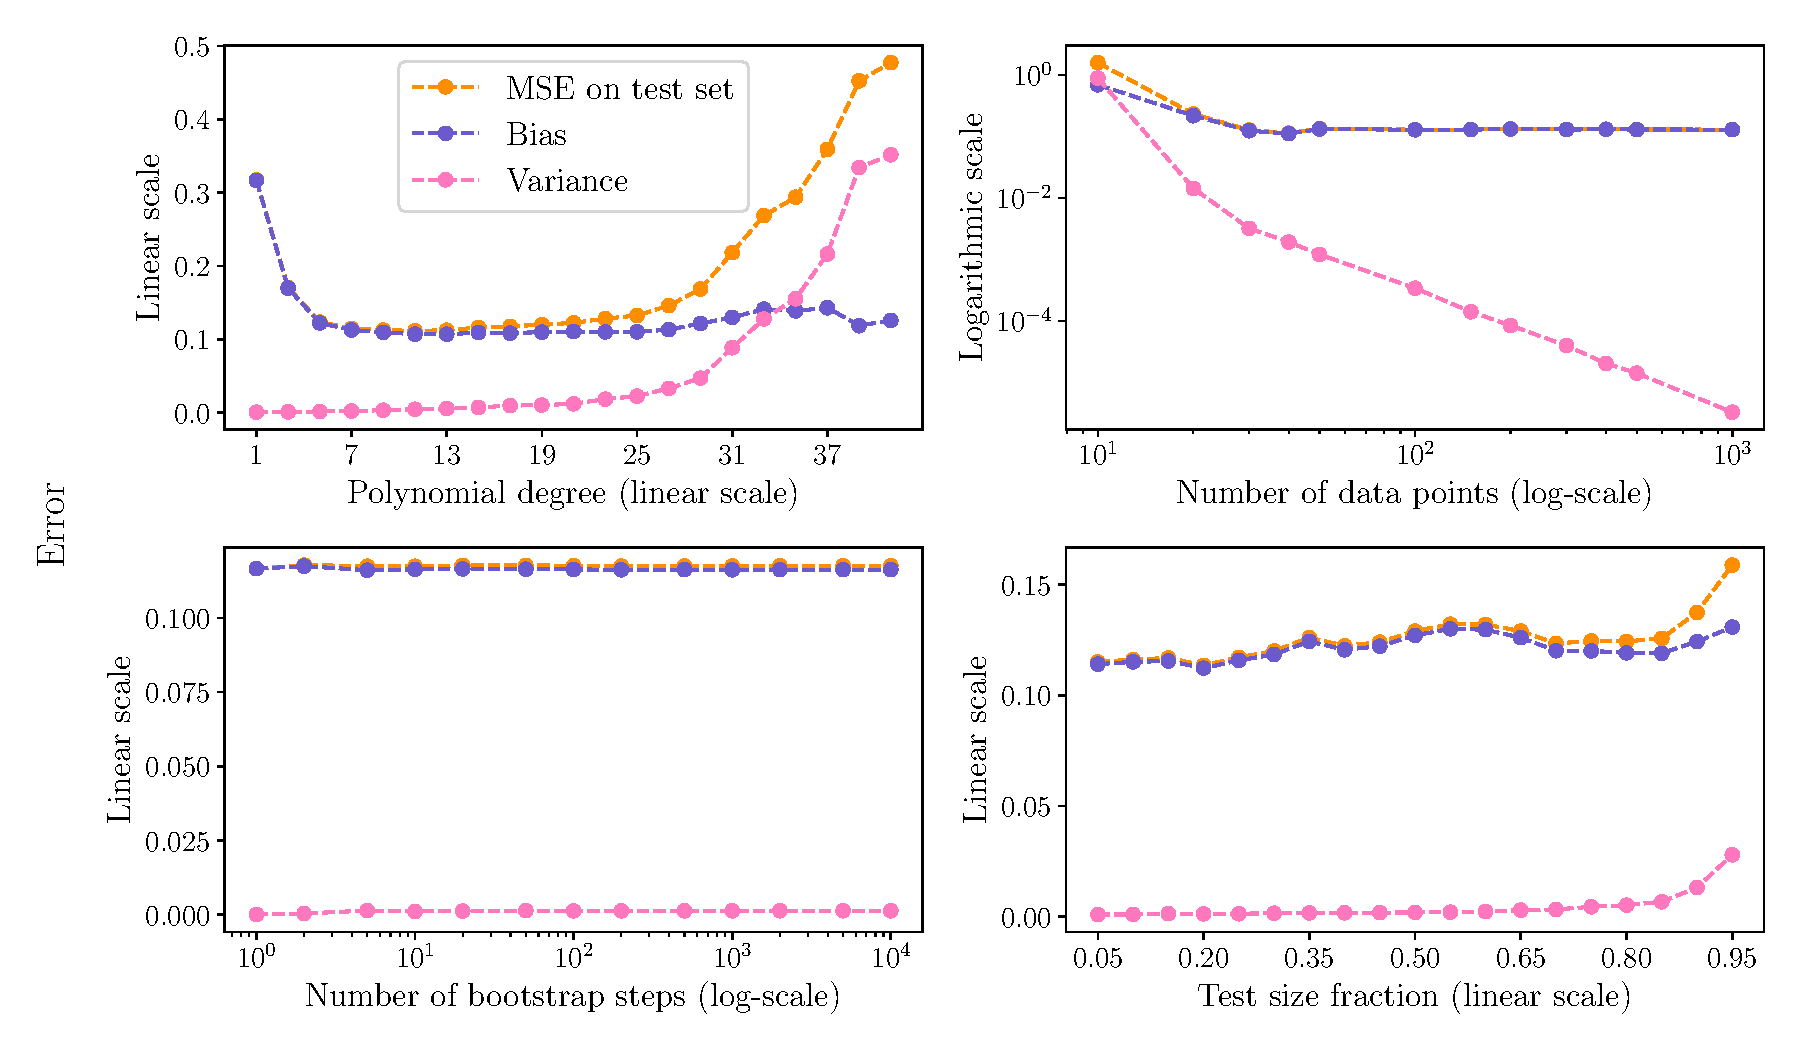
\includegraphics[width=\textwidth]{../figs/e_bias_variance.pdf}
  \caption{MSE (orange), bias (blue) and variance (pink) for OLS regression evaluated on Franke test data and plotted as functions of polynomial degree (upper left), number of data points (upper right), number of bootstrap steps (lower left) and test size fraction (lower right). When these are not varied we have used degree 5, $50\times50$ data points, 100 bootstrap steps and a test size fraction of 0.2. Note that some axes are scaled logarithmically and some have a linear scale.}\label{fig:e bias variance}
  \vspace*{-5pt}
\end{figure*}

The bias-variance tradeoff is clearly showcased, since the bias and MSE stabilize at their lowest value of around 0.1 at polynomial degree 7, where the variance is still very low. As we move towards degrees $>19$ the steady increase in variance picks up while the bias remains more or less the same, and as a result the MSE starts increasing again. 

We see that increasing the number of data points in the grid past $50\times50$ has little to no effect on the bias, while the variance falls to zero. This is because the bias is determined by the model's assumptions about the underlying data structure, i.e. its complexity, and not by the amount of training data. On the other hand, model variance decreases with the number of data points because the model becomes less sensitive to fluctuations in individual data points. This is because the model is trained on a dataset that is more representative of the true underlying data distribution, which reduces the likelihood of the model fitting to random noise or outliers that are not reflective of the true relationship between the features and the target variable. 

Both the bias and the variance increase as we move to the extreme case of reserving more than 90\% of the data for testing, since we then have very few data points to train the model with. This heightens the chance of fitting to random fluctuations due to noise, which leads to an increased variance, as well as the probability of not having enough data points to capture the complex nature of the dataset's underlying structure, which increases the bias. We suspect that the error would be even larger had it not been for bootstrapping, since this typically minimizes the variance when working with a very small dataset. Moreover, increasing the number of bootstrap steps does not seem to be necessary when using a polynomial degree of 5 and $50\times50$ data points, since both the bias and the variance remain practically constant. This agrees well with the complexity dependency plot, since the variance was negligible for this degree, and bootstrapping generally does not help with decreasing the bias. For future studies on the bias-variance tradeoff it would be interesting to see how the dependency on the number of bootstrap steps would change if we used a polynomial degree of e.g. 40 instead. 

Comparing \cref{fig:e train test} and the top left subplot in \cref{fig:e bias variance} we see that the MSE evaluated on the test set stays more or less constant at $\lesssim0.15$ for polynomial degrees $\in[20,70]$ when not employing bootstrap, while it increases past this value as we move to degrees $>20$ when using 100 bootstrap steps. The reason for this is that bootstrapping actually can lead to an increased model variance if the dataset is already large enough, because in that case the model already captures most of the data's inherent variability. Bootstrapping, which samples with replacement, results in some data points being included multiple times and others being left out in each resampled dataset. This can create redundant patterns that the model may pick up on. In large datasets, these redundant patterns are more likely to differ across bootstrapped samples, potentially leading to fluctuations in the fitted model. Thus, we hypothesize that a $50\times50$ dataset was large enough, and that increasing the polynomial degree to around 40 would lead to an increase in variance and MSE with the number of bootstrap steps.


\subsection{Resampling Methods}
\subsubsection{OLS: Cross-Validation VS Bootstrap}
In the top (bottom) part of \cref{fig:kfold vs bootstrap} we have plotted OLS model MSE's evaluated on Franke (cosmological) test data against polynomial degrees $\in[1,15]$ ($\in[1,31]$). In the left column we have MSE's estimated from cross-validation, and the number of $k$-folds used vary in integer steps between 5 and 15. In the right column we have plotted their MSE's computed using 100 bootstrap steps. We did not vary the number of steps as we did $k$, because we assumed from \cref{fig:e bias variance} that the dependency on the number of steps would be miniscule. As mentioned in the previous section this might not be the case, though, and in further investigation it may prove insightful to explore this dependency as well.


\begin{figure*}
  \vspace*{-5pt}
  \centering %Centers the figure
  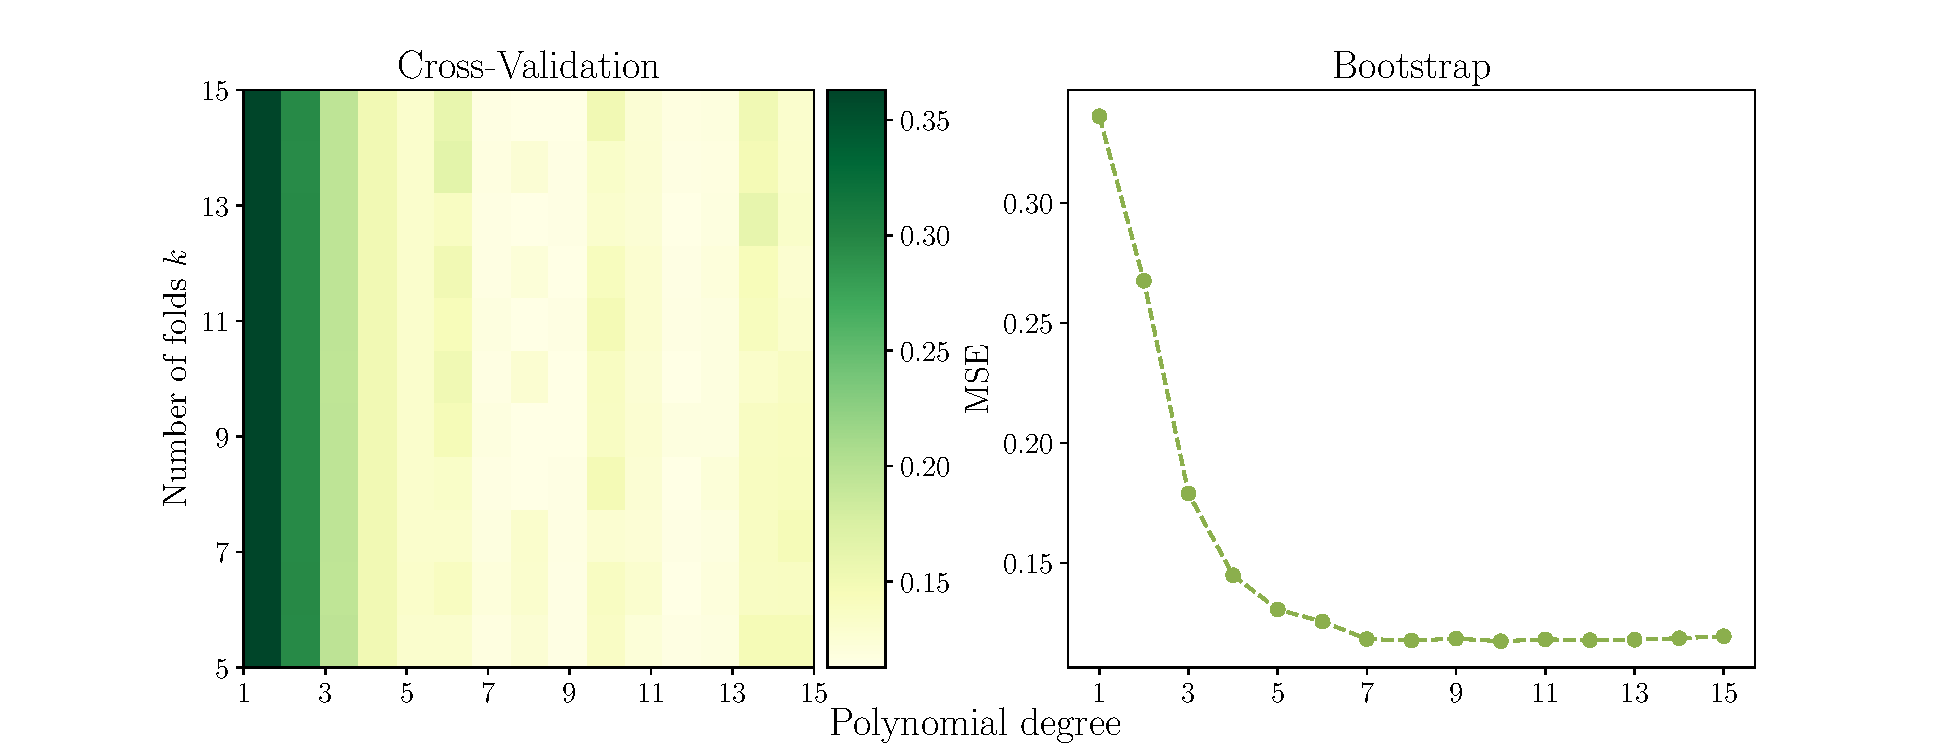
\includegraphics[trim = 0 0.8cm 0 0,clip,width=0.95\textwidth,keepaspectratio]{../figs/f_kfold_vs_bootstrap.pdf}
  \centering
  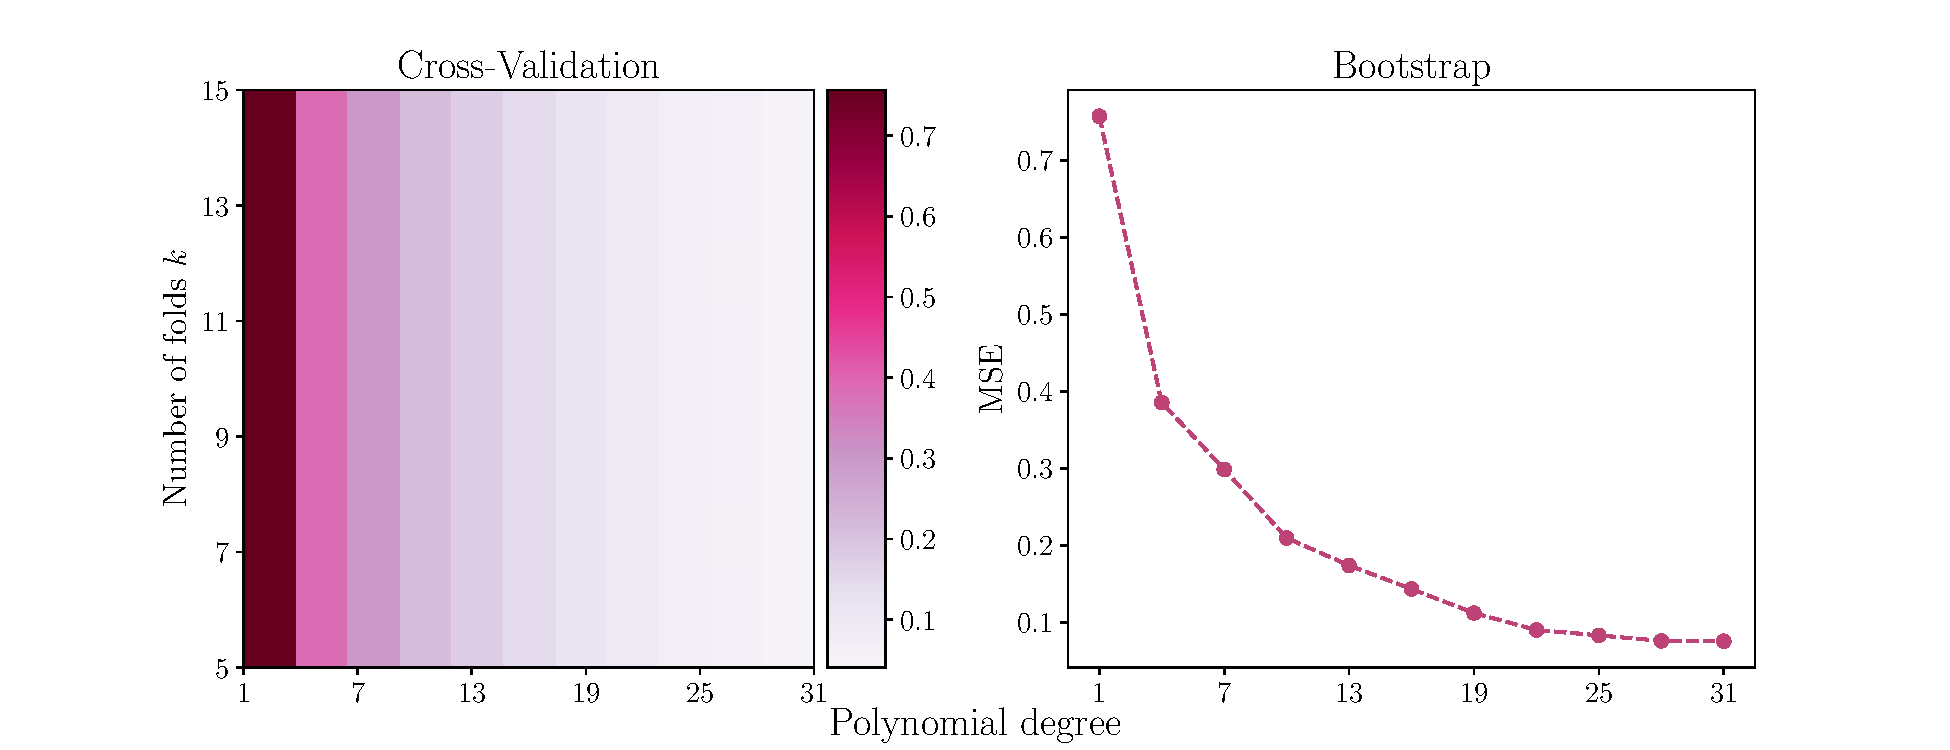
\includegraphics[width=0.95\textwidth]{../figs/g_kfold_vs_bootstrap.pdf}
  \caption{MSE evaluated on Franke (upper row) and cosmological (lower row) test data as function of polynomial degrees in the intervals $[1,15]$ (Franke) and $[1, 31]$ (cosmological) and number of folds $k\in[5, 15]$ used in cross-validation (contour plots on the left). On the right we have plotted the MSE's purely as functions of complexity when using the bootstrap resampling method with 100 steps.}\label{fig:kfold vs bootstrap}
  \vspace*{-5pt}
\end{figure*}

Assuming our predictions of the bootstrap dependency is correct, the observed dependency on the number of $k$-folds is not surprising, since the former would suggest that the models are relatively insensitive to fluctuations in the training set as is. Cross-validation would then be rather ineffective in further minimizing the model variance, since the dataset is probably large or homogeneous enough that the way it is split does not lead to a substantial difference in the training or validation sets. Furthermore, we see that for the Franke data the MSE fluctuates somewhat with $k$ for polynomial degrees $\gtrsim7$, especially for degrees 8 and 14. The fluctuations are small and seem to follow a somewhat random pattern, however, and are most likely not very telling of the fits' relative qualities. This should be tested more extensively before saying for sure, though.

For the dark matter simulation data, $k$-fold cross-validation appears to be rather ineffective at reducing the model error, since there is no visible dependency on the number of folds. In fact, the decrease in MSE with complexity seems to be more or less the same for both cross-validation and bootstrap, and the fact that the MSE's flatten out only as we reach degrees $\gtrsim25$ implies that we have not yet reached the model complexity that properly captures the variability of our data. In other words, the main contribution to the model error for the lower polynomial degrees is bias due to underfitting rather than the variance, which neither cross-validation nor bootstrap can minimize to any significant degree. We did not explore higher complexities due to the increasingly long computational time, but this would definitely be a leading topic of further investigation. 


\subsubsection{Cross-Validation With Ridge and Lasso}
The blue-green (brown-yellow) contour plots in \cref{fig:kfold Ridge Lasso} show the MSE scores of fits to the Franke generated data as well as the cosmological simulation data using Ridge (Lasso) regression. The MSE's for the Franke and cosmological fits are plotted in the top and bottom sections, respectively, and the plots on the left (right) correspond to $\lambda=0.001$ ($\lambda=0.5$). We have used the same range of polynomial degrees and $k$'s here as for the OLS case plotted in \cref{fig:kfold vs bootstrap}. It is important to note the scale on the bottom right plot, which shows that the MSE scores fluctuate around 1 with an order of magnitude $\lesssim10^{-7}$. 

\begin{figure*}
  % \vspace*{-5pt}
  \centering %Centers the figure
  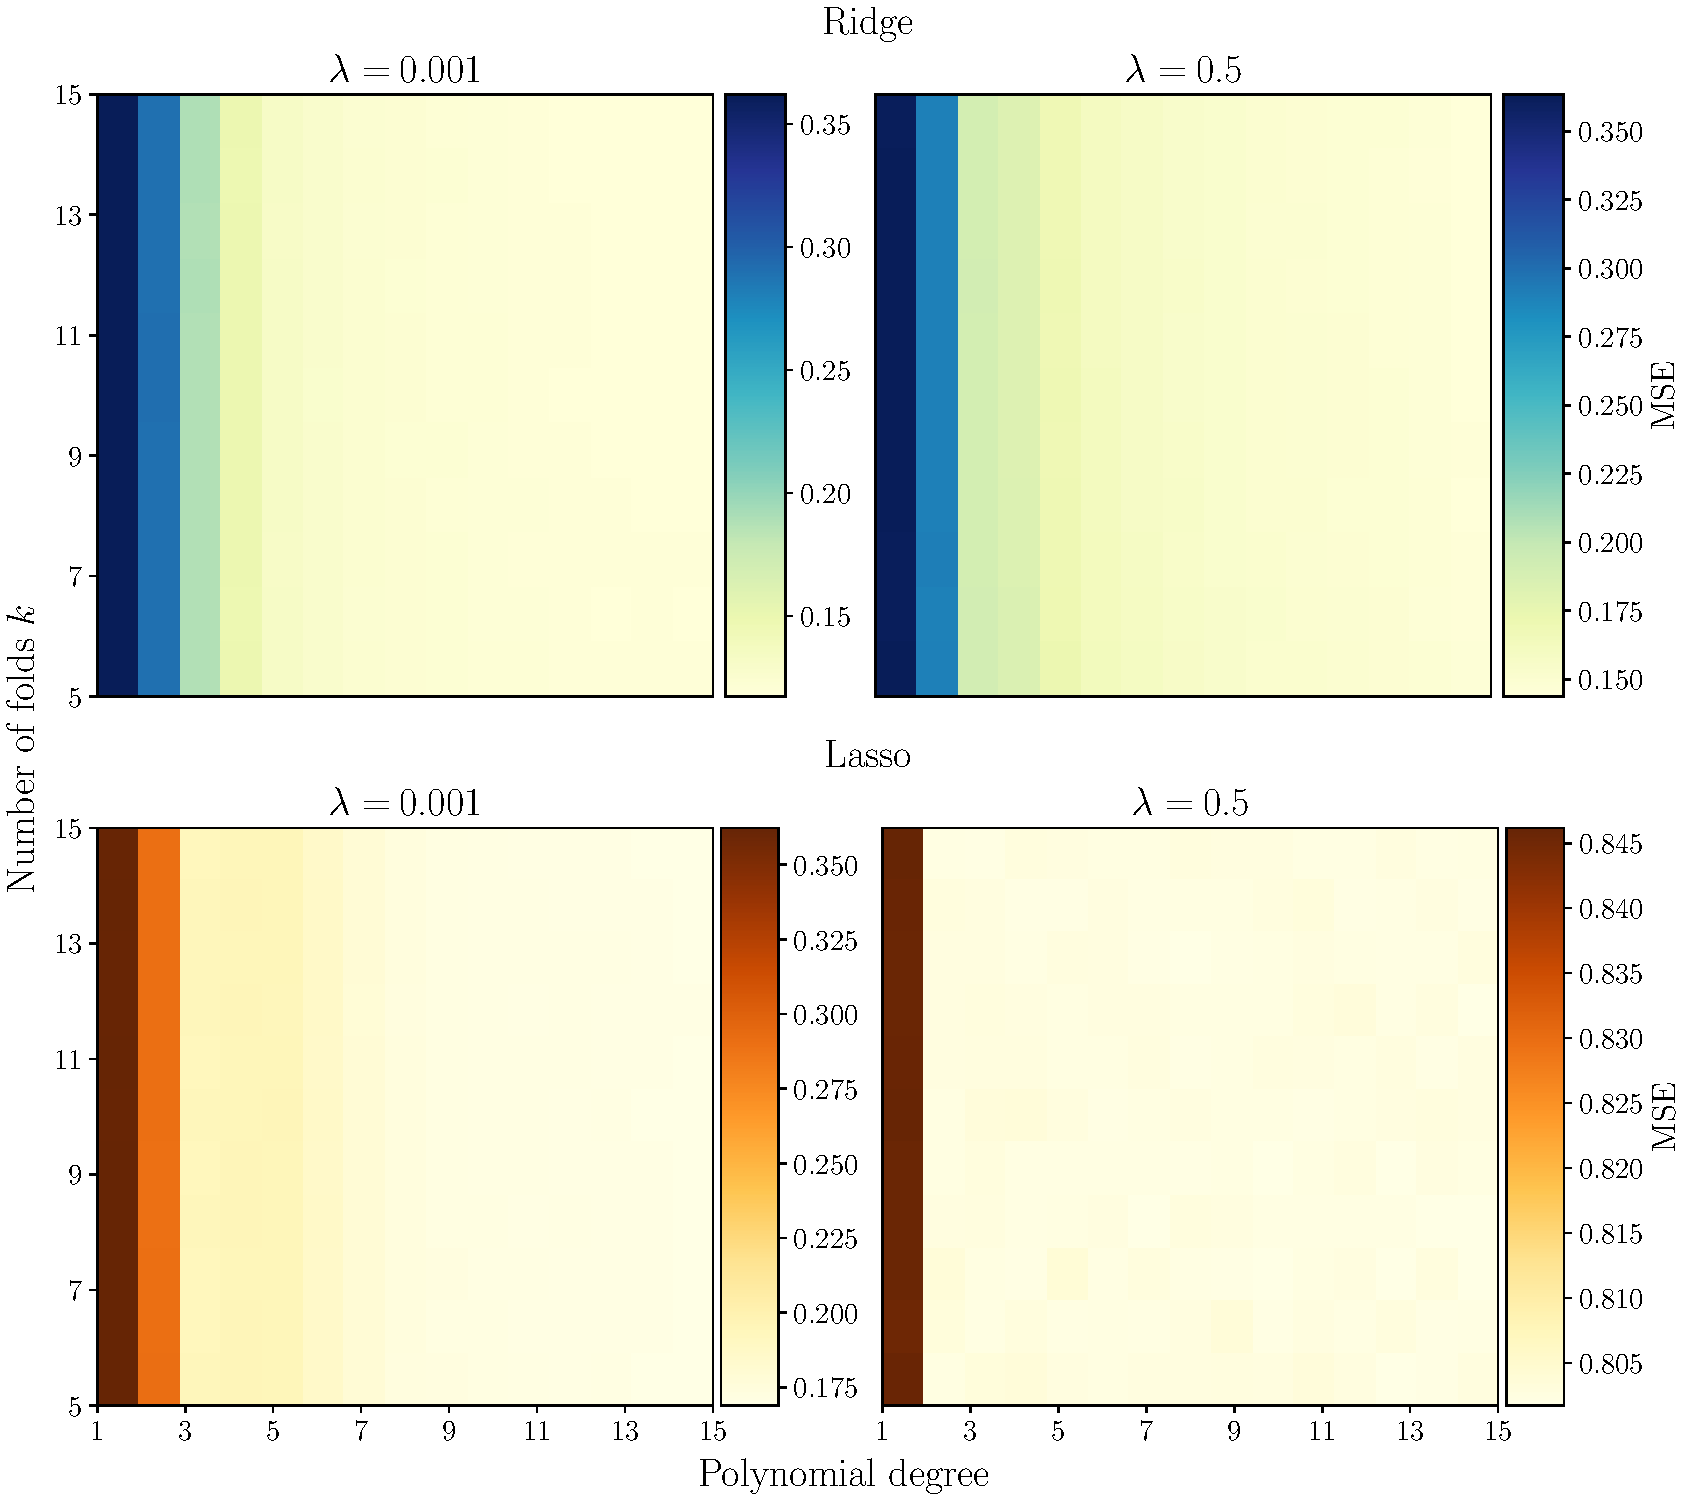
\includegraphics[width=0.7\textwidth]{../figs/f_Ridge_Lasso.pdf}
  \centering
  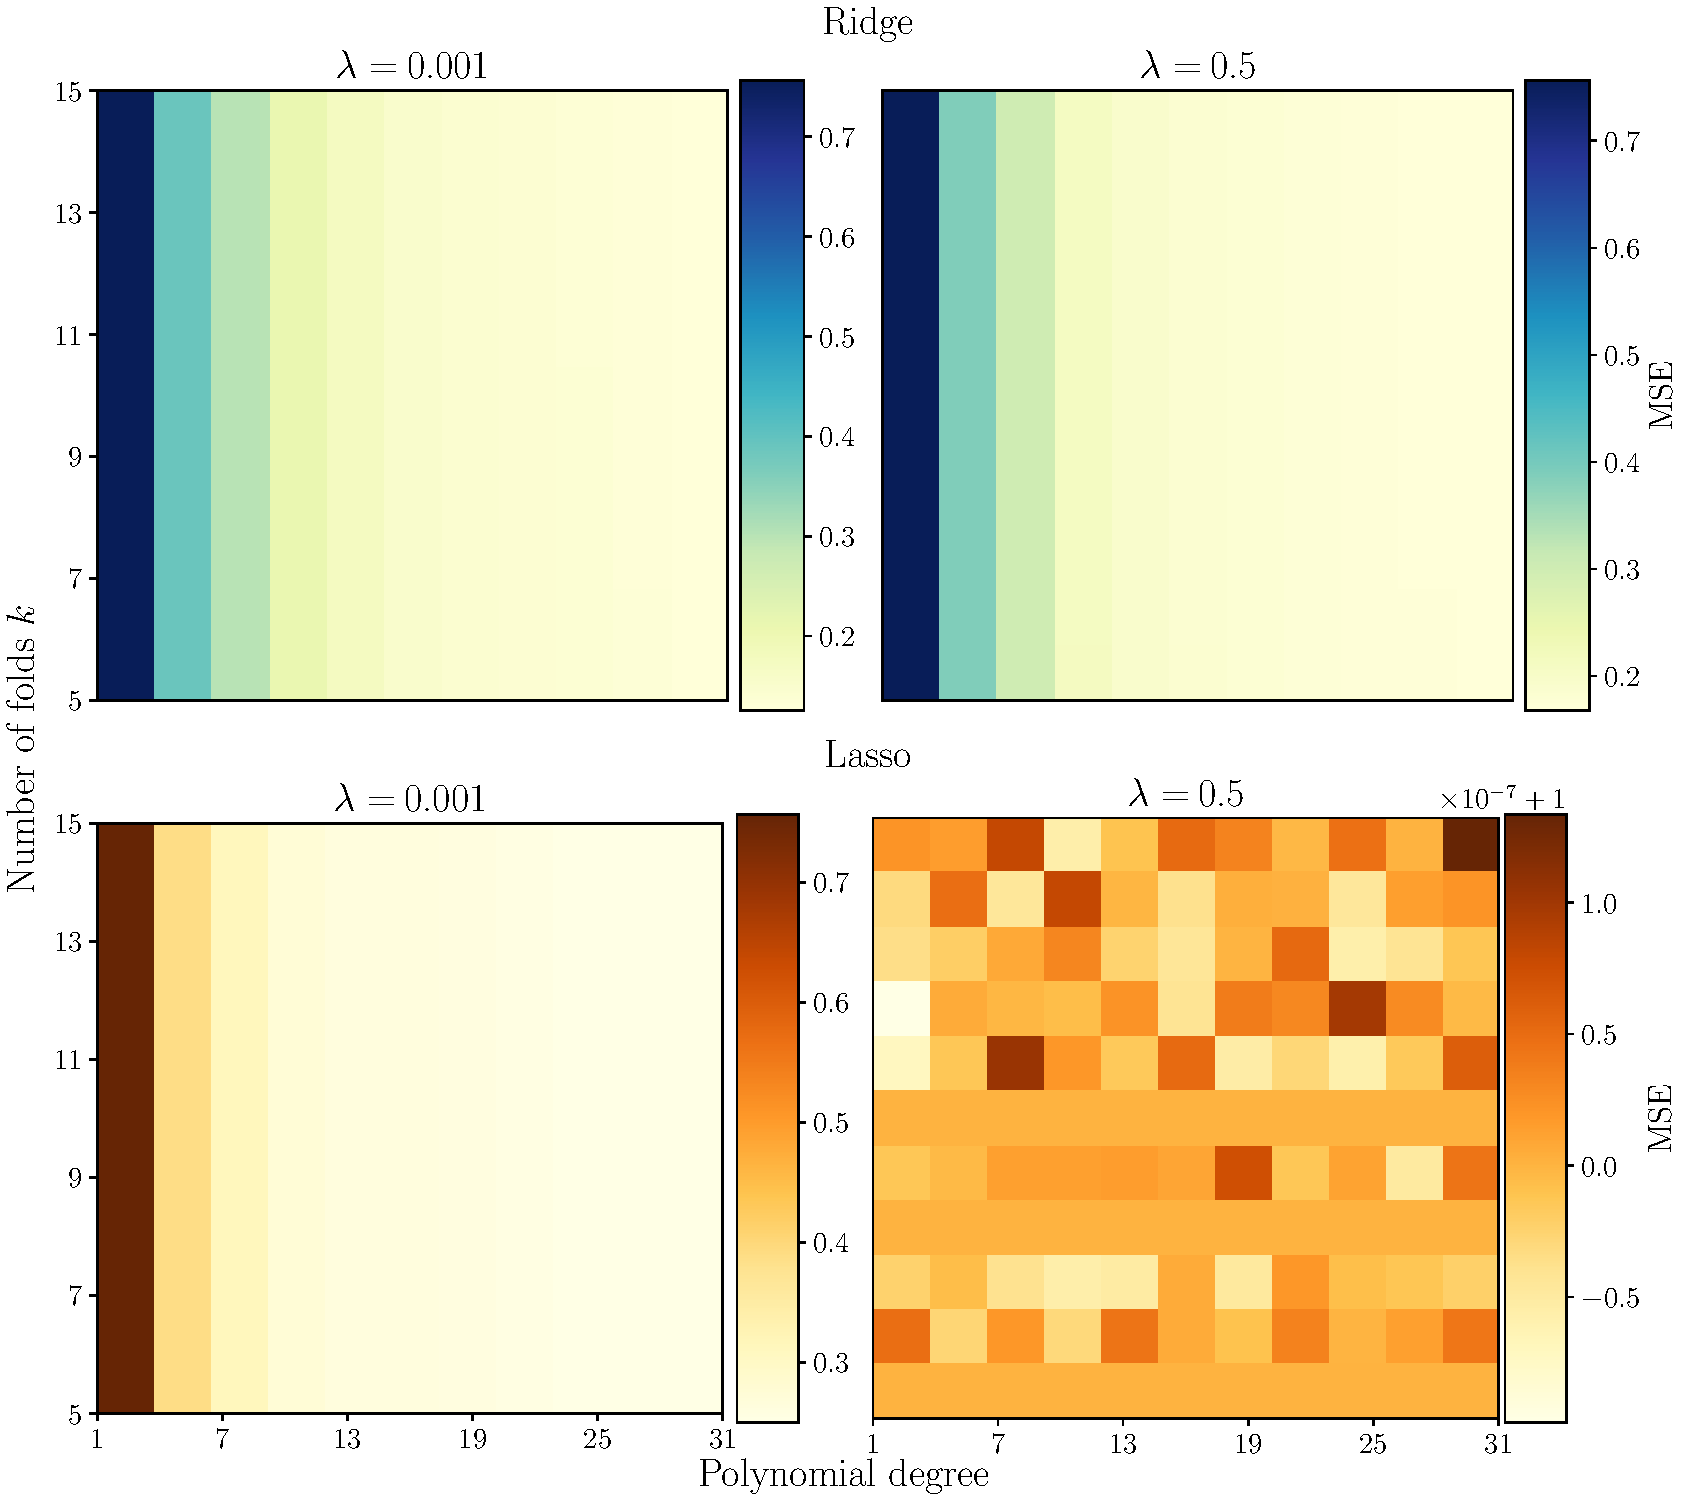
\includegraphics[width=0.7\textwidth]{../figs/g_Ridge_Lasso.pdf}
  \caption{MSE evaluated on the Franke (top section) and cosmological (bottom section) test sets as function of polynomial degrees and number of $k$-folds used in cross-validation, for Ridge (upper rows) and Lasso (lower rows) regression. We have used $\lambda=0.001$ and $\lambda=0.5$ in the left and right columns, respectively.}\label{fig:kfold Ridge Lasso}
  % \vspace*{-5pt}
\end{figure*}

Based on our discussions in \cref{subsec:hyperparameter} it is not surprising that the Ridge fits' MSE's are more or less the same for both hyperparameters, while the Lasso MSE's are significantly larger for $\lambda=0.5$ than $\lambda=0.001$. Nor is it suprising that varying the number of $k$-folds have negligible effect on the scores. In fact, by introducing a regularization term as we do with Ridge and Lasso regression we actually undermine the model complexity even further, which is probably why the small MSE fluctuations observed for OLS on the Franke data are not present here. Again, in further analyses it would be interesting to explore how the scores change as we increase the polynomial degrees, specifically at what points introducing a regularization term starts to prove useful and the number of $k$-folds has a visible effect.


\subsection{Fits to the Cosmological Data}
\subsubsection{Complexity Dependency in OLS}
In \cref{fig:density complexity} we have plotted OLS fits to the cosmological data using polynomial degrees 5, 10, 20, 30 and 50 to further examine the effects of increasing model complexity. From degree 30 to 50 the fit actually seems to worsen, looking more smudged in the center, while ripple-like structures near the edges become more prominent. These are already visible for degree 30, especially in \cref{appfig:density surf} in \cref{appsec:figures}, where we have surface plotted the fit together with the actual data.

To explain the reason for the ripple effect, and why the smaller scale structures in the data don't show up more clearly as we continue increasing the model complexity, we need to consider the columns of the scaled design matrix. As mentioned in \cref{subsec:scaling effect} most of the scaled box coordinates are less than 1. They are in fact close to zero in the center region and slightly larger than 1 in magnitude near the edges. Thus, as we move to higher order polynomials the elements of the rightmost columns in $\mathbf{X}_\text{scaled}$ (corresponding to the highest order terms) diverge, some tend to zero while others grow in magnitude. To minimize the model error the coefficients cannot continue increasing because then the fit worsens in the edges, but they cannot decrease too much either as this leads to a less accurate fit in the center. As a result we see the fits become increasingly smeared in the center and more complex at the edges as we increase the complexity.

\begin{figure*}
  \vspace*{-5pt}
  \centering %Centers the figure
  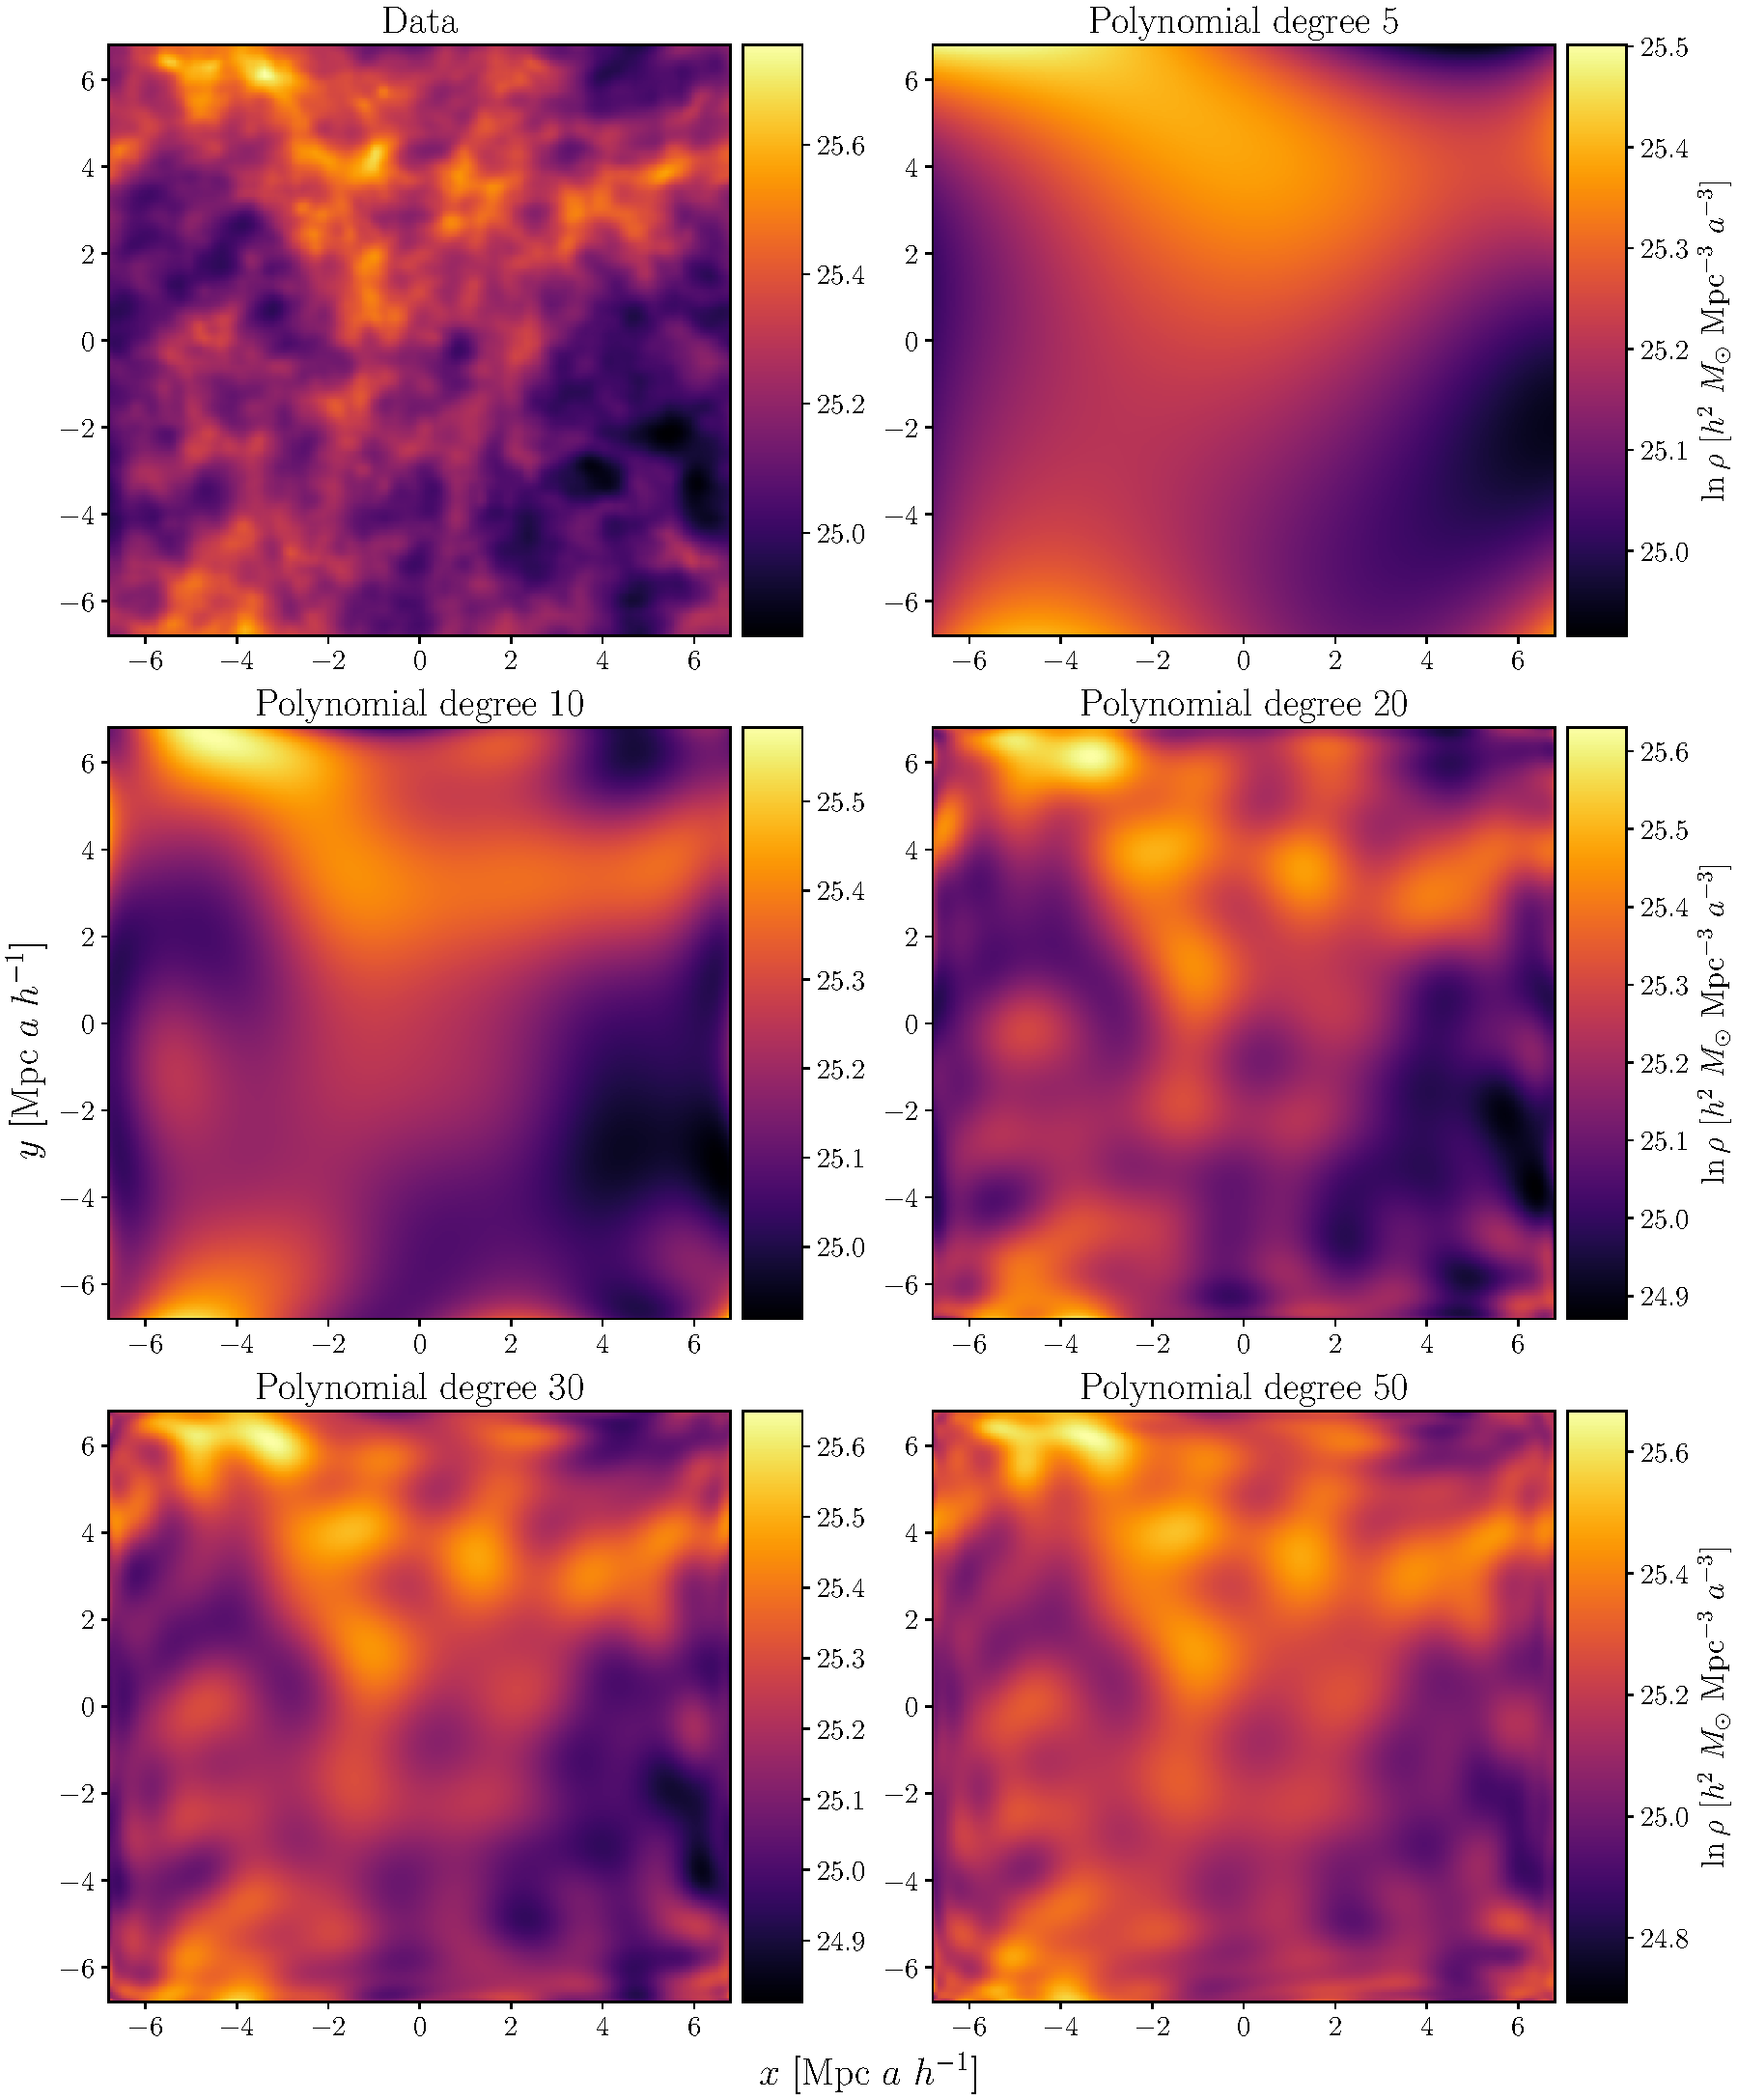
\includegraphics[width=0.85\textwidth]{../figs/density_complexity.pdf}
  \caption{Contour plots of the cosmological simulation data (upper left) and the OLS fits for polynomial degrees 5 (upper right), 10 (middle left), 20 (middle right), 30 (lower left) and 50 (lower right).}\label{fig:density complexity}
  \vspace*{-5pt}
\end{figure*}

In an attempt to confirm this interpretation we decided to split our simulation data into equally sized pieces, scale each piece and perform fits on them separately, then stitch them back together. That way, we hypothesized that the smearing and ripple effects would be minimized and more evenly distributed through the grid since the complex structure of the data is simpler on smaller, local scales. We did this with 4 pieces and 100 pieces, using OLS and polynomial degree 30 in both cases, and the result is shown in \cref{appfig:density pieces} in \cref{appsec:figures}. Indeed, we see that the resulting fit with 100 pieces looks nearly identical to the actual data. For the fit with 4 pieces it is very obvious that we have stitched separate fits back together, since we clearly see the ripple effects from each fit meeting at the boundaries.



\subsubsection{Comparing Regression Variants}
In \cref{fig:density OLS Ridge Lasso} we have plotted the OLS, Ridge and Lasso fits using polynomial degree 30, hyperparameter  $\lambda=0.001$ and $k=5$ folds together with the actual data to get a feel for the implications of the estimated MSE scores. Here we see that the Lasso fit is significantly worse than both OLS and Ridge, although Ridge is lacking in comparison to OLS as well. This agrees with figs. \ref{fig:kfold vs bootstrap} and \ref{fig:kfold Ridge Lasso}, since the MSE's for the largest plynomial degrees lie somewhere below 0.1 for OLS, in the interval $[0.1,0.2]$ for Ridge and $[0.2,0.3]$ for Lasso. It also makes sense considering the scores plotted in \cref{appfig:g MSE R2} in \cref{appsec:figures}, where we saw that Lasso generally performed poorly compared to Ridge.

\begin{figure*}
  \vspace*{-5pt}
  \centering %Centers the figure
  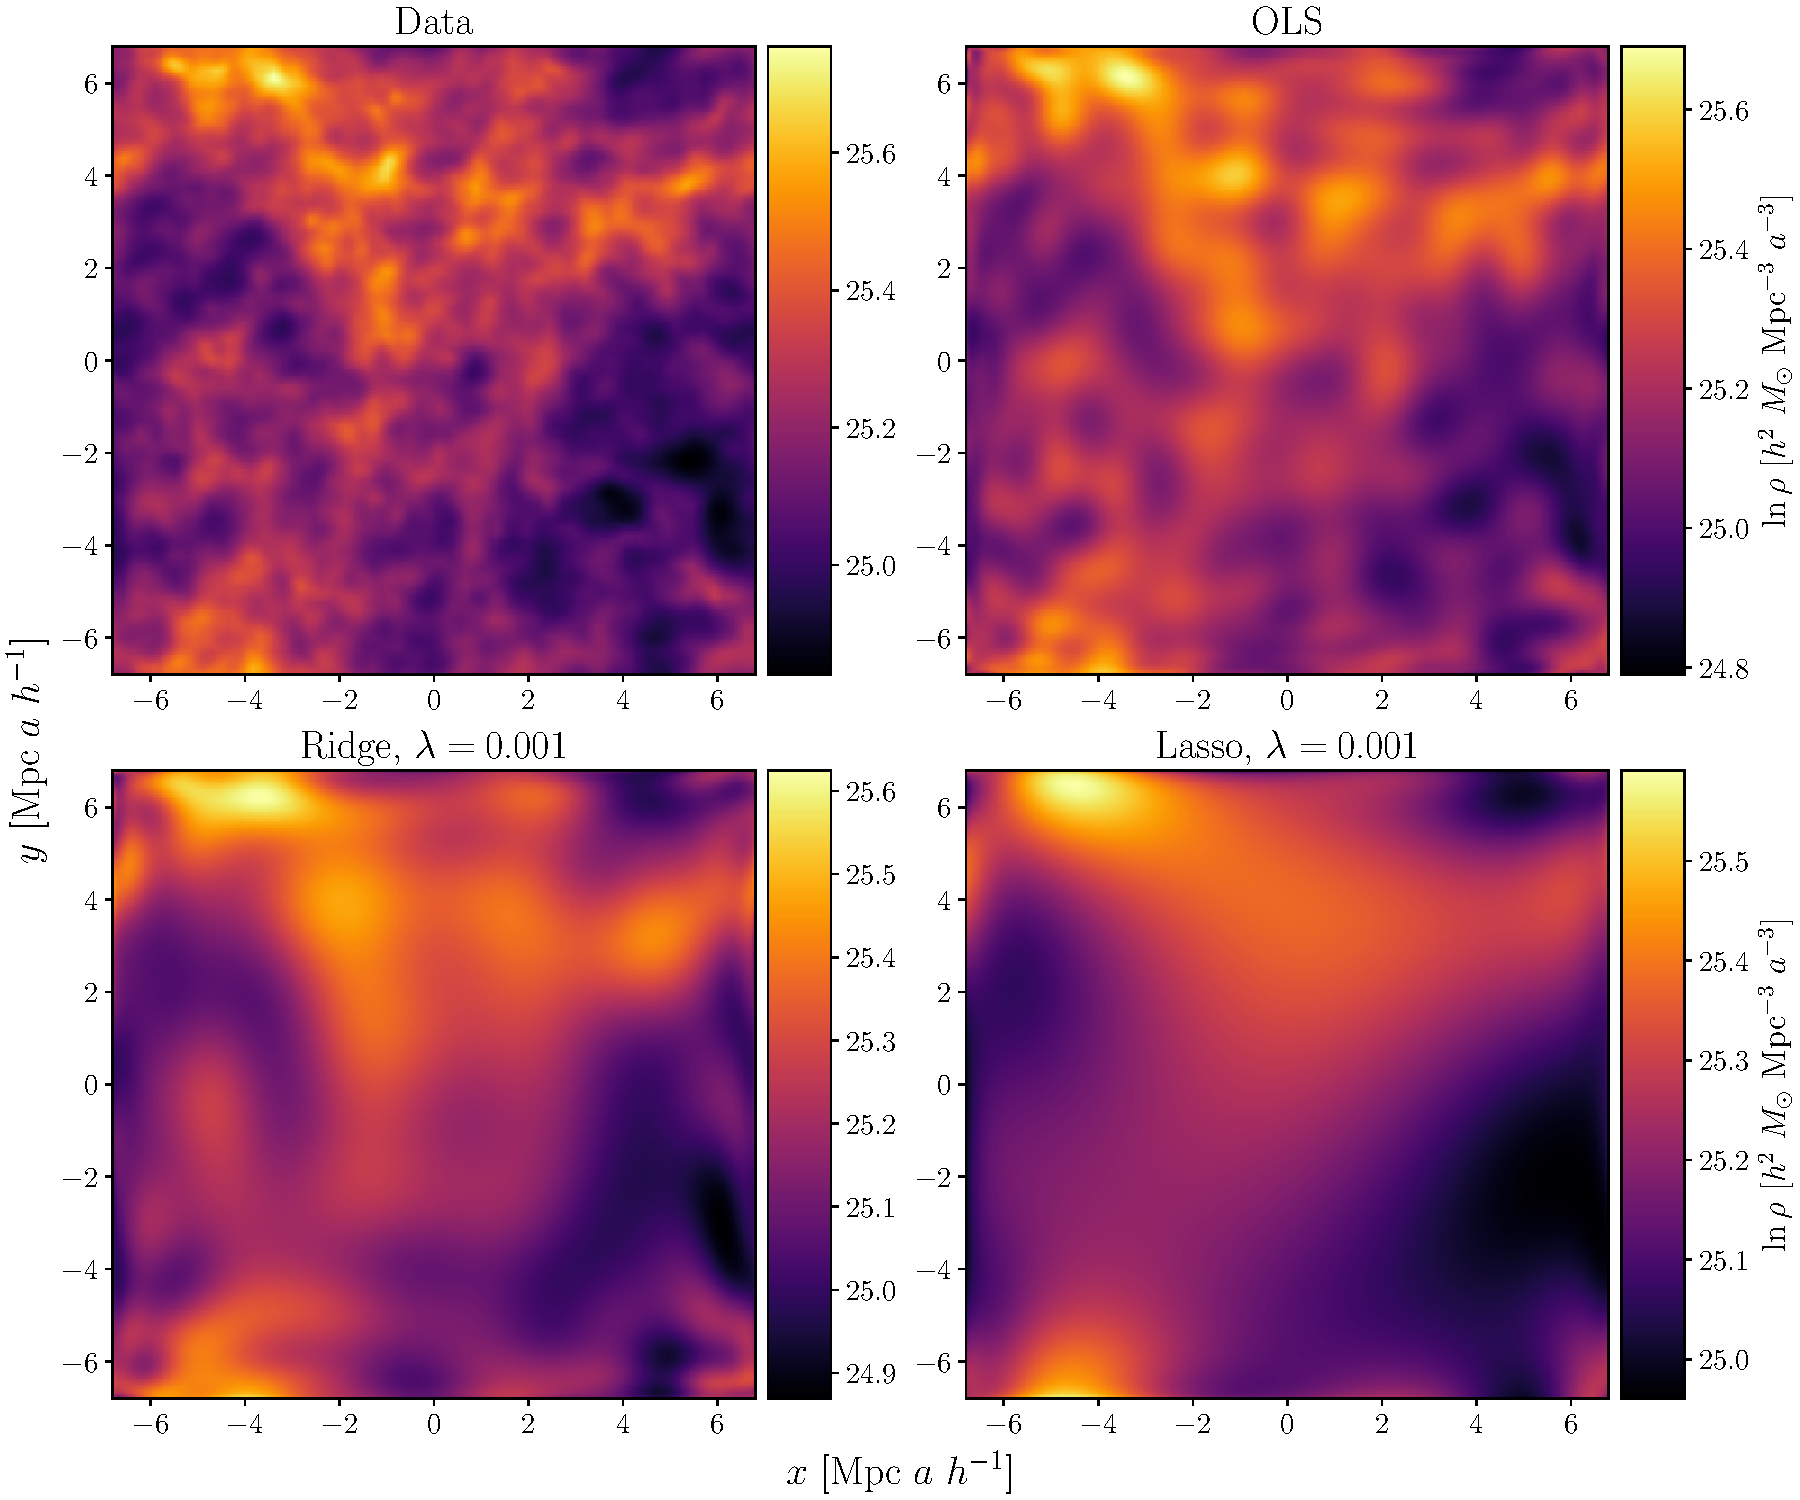
\includegraphics[width=0.85\textwidth]{../figs/density_OLS_Ridge_Lasso.pdf}
  \caption{Contour plots of the cosmological simulation data (upper left) and OLS (upper right), Ridge (lower left) and Lasso (lower right) regression fits using polynomial degree 30, $\lambda=0.001$ for both Ridge and Lasso, and $k=5$ folds in cross-validation.}\label{fig:density OLS Ridge Lasso}
  \vspace*{-5pt}
\end{figure*}

It is not surprising that OLS worked best with our chosen polynomial degree, since we are far from reaching the complexity of the actual data. Thus, introducing a penalizing regularization term when computing the estimators $\boldsymbol{\hat{\beta}}$ to account for overfitting is of little use, and the result is instead that the fits become too simplistic. In order to understand why the Lasso fit is so poor compared to the Ridge fit we need to review their cost functions. The $L^1$ norm used in Lasso regression creates a sparser model by shrinking some coefficients entirely to zero, which tends to be more pronounced when dealing with higher polynomial degrees where many coefficients could have minimal or redundant contributions to the model. The $L^2$ norm in Ridge regression penalizes large coefficients as well, but does not drive them to zero. While it still reduces the impact of large polynomial coefficients, it tends to be less severe in its penalization than Lasso, particularly for coefficients that contribute significantly to the model.


% \vspace*{-2.5pt}
\section{Conclusion}\label{sec:conclusion}
% \vspace*{-2.5pt}
In this study we have implemented and compared three well known regression techniques - Ordinary Least Squares (OLS), Ridge, and Lasso - in the context of both synthetic and real world data. We employed the widely used Franke function to generate the former, which we used to validate our implementations and explore fundamental concepts in machine learning such as the bias-variance tradeoff. Our investigation of Ridge and Lasso regression revealed that adding regularization terms to the cost function, which is known to be an effective way to overfitting, either reduced the model performances or left them unchanged. We concluded that our dataset contained enough points for the models to be able to fit to its underlying structure without fitting to the noise, even as we increased the model complexity way past what was necessary. This was validated by the application of two well known resampling methods; bootstrap and $k$-fold cross-validation, as these typically minimize model variance due to overfitting, but had minimal obervable effect on our model errors. 

Our analyses were further extended to cosmological N-body simulation data generated with the public version of the G\begin{scriptsize}ASOLINE\end{scriptsize}2 SPH code. Due to runtime constraints we repeated the aforementioned analyses only for polynomial degrees $\in[1,31]$, even though the variability of the data indicated that we should explore even more complex models. This revealed that introducing regularization only worsened the model performances, while bootstrapping and cross-validation had negligible visible effect. These results were not surprising based on our previous analyses of the Franke function data since the cosmological data is significantly more complex, and we did not add any random noise components. Increased errors due to overfitting with polynomial degree 31 would be a peculiar result when we observed that this did not happen for the Franke function data before we reached polynomial degrees $\gtrsim70$. 

We observed with OLS that employing a polynomial degree larger than 20-30 lead to a ripple-like effect near the edges of the grid while still not accounting for the complex structure in the center. In future work it would be interesting to explore more advanced regularization techniques combined with even larger polynomial degrees to see if we could mitigate the effect. We would also have to direct our focus towards code optimization in order to reduce the limiting computation time.

% \section*{Acknowledgements}\label{sec:cknowledgements}
% % MAYBE REMOVE

\Urlmuskip=0mu plus 1mu\relax
\onecolumngrid
\bibliography{references}

\newpage
% ===========================================
\appendix
\section{Code}\label{appsec:code}
Link to our GitHub repository: \href{https://github.com/Oskar-Idland/FYS-STK4155-Projects}{https://github.com/Oskar-Idland/FYS-STK4155-Projects}

\section{Derivations}\label{appsec:derivations}
\subsection{Expectation value and variance of the OLS estimator \texorpdfstring{$\boldsymbol{\hat{\beta}}$}{Lg}}\label{subapp:beta OLS}
Since the error in $\mathbf{y}$ is normal distributed as $\boldsymbol{\varepsilon}\sim N(0,\sigma^2)$ we know that the expectation value and variance of the $i$'th element of $\boldsymbol{\varepsilon}$ is $\mathbb{E}(\varepsilon_i)=0$ and $\textrm{Var}(\varepsilon_i)=\sigma^2$. Thus, since we approximate $f(\mathbf{x})$ with $\mathbf{\tilde{y}}=\mathbf{X}\boldsymbol{\beta}$ the expectation value of $\mathbf{y}$ becomes 
\begin{equation}
\mathbb{E}(\mathbf{y})=\mathbb{E}(\mathbf{X}\boldsymbol{\beta}) + \mathbb{E}(\boldsymbol{\varepsilon}) = \mathbb{E}(\mathbf{X}\boldsymbol{\beta}),
\end{equation}
which gives us the expectation value of $\mathbf{y}$ for a given element $i$:
\begin{equation}
\mathbb{E}(y_i) = \mathbb{E}\left(\sum_jX_{ij}\beta_j\right) = \sum_jX_{ij}\beta_j = \mathbf{X}_{i,*}\boldsymbol{\beta}.
\end{equation}
Here we have used that the sum $\sum_jX_{ij}\beta_j$ is known to be the value of $\tilde{y}_i$, hence its expectation value is itself. Moreover, we can similarly find the variance of $\mathbf{y}$ for a given element $i$ by using that the terms in the aforementioned sum are known to be $\tilde{y}_i$ for all $i$, i.e. $\textrm{Var}(\mathbf{X}_{i,*}\boldsymbol{\beta})=0$. Thus, we have
\begin{equation}
\textrm{Var}(y_i) = \textrm{Var}(\mathbf{X}_{i,*}\boldsymbol{\beta}) + \textrm{Var}(\varepsilon_i) = \sigma^2,
\end{equation}
and consequently
\begin{equation}
  y_i\sim N(\mathbf{X}_{i,*}\boldsymbol{\beta},\sigma^2).
\end{equation}
Now, using that the OLS estimator is given by $\boldsymbol{\hat{\beta}}=\left(\mathbf{X}^\top\mathbf{X}\right)^{-1}\mathbf{X}^\top\mathbf{y}$, its expectation values become
\begin{align*}
  \mathbb{E}(\boldsymbol{\hat{\beta}})&=\mathbb{E}\left\{ \left(\mathbf{X}^\top\mathbf{X}\right)^{-1}\mathbf{X}^\top\mathbf{y} \right\} \\
  &= \mathbb{E}\left\{\left(\mathbf{X}^\top\mathbf{X}\right)^{-1}\mathbf{X}^\top\right\} \mathbb{E}(\mathbf{y}) \\
  &= \left(\mathbf{X}^\top\mathbf{X}\right)^{-1}\mathbf{X}^\top\mathbf{X}\boldsymbol{\beta} \\
  &= \boldsymbol{\beta}. \numberthis \label{appeq:expect beta OLS}
\end{align*}
Furthermore, if $x$ and $y$ are two independent variables, the variance of their product is given by
\begin{align*}
\textrm{Var}(xy) &= \mathbb{E}(x^2y^2)-(\mathbb{E}(xy))^2, \\
&= \mathbb{E}(x^2)\mathbb{E}(y^2) - \left(\mathbb{E}(x)\right)^2\left(\mathbb{E}(y)\right)^2,
\\
&= \left[\mathbb{E}(x^2) - \left(\mathbb{E}(x)\right)^2 + \left(\mathbb{E}(x)\right)^2\right]\left[\mathbb{E}(y^2) - \left(\mathbb{E}(y)\right)^2 + \left(\mathbb{E}(y)\right)^2\right] - \mathbb{E}(x^2)\mathbb{E}(y^2),
\\
&= \left[\textrm{Var}(x) + \left(\mathbb{E}(x)\right)^2\right]\left[\textrm{Var}(y) + \left(\mathbb{E}(y)\right)^2\right] - \mathbb{E}(x^2)\mathbb{E}(y^2), \\
&= \textrm{Var}(x)\textrm{Var}(y) + \textrm{Var}(x)(\mathbb{E}(y))^2 + \textrm{Var}(y)(\mathbb{E}(x))^2 +\mathbb{E}(x^2)\mathbb{E}(y^2)- \mathbb{E}(x^2)\mathbb{E}(y^2),
\\
&= \textrm{Var}(x)\textrm{Var}(y) + \textrm{Var}(x)(\mathbb{E}(y))^2 + \textrm{Var}(y)(\mathbb{E}(x))^2,
\end{align*}
so if we now set $x=\left(\mathbf{X}^\top\mathbf{X}\right)^{-1}\mathbf{X}^\top$ and $y=\mathbf{y}$ we find that the variance of $\boldsymbol{\hat{\beta}}$ is
\begin{align*}
\textrm{Var}(\boldsymbol{\hat{\beta}}) 
&= \underbrace{\textrm{Var}\left[\left(\mathbf{X}^\top\mathbf{X}\right)^{-1}\mathbf{X}^\top\right]\textrm{Var}(\mathbf{y})}_0 
+ \underbrace{\textrm{Var}\left[\left(\mathbf{X}^\top\mathbf{X}\right)^{-1}\mathbf{X}^\top\right](\mathbb{E}(\mathbf{y}))^2}_{0} 
+ \textrm{Var}(\mathbf{y})\left(\mathbb{E}\left[\left(\mathbf{X}^\top\mathbf{X}\right)^{-1}\mathbf{X}^\top\right]\right)^2,
\\
&= \sigma^2\left[\left(\mathbf{X}^\top\mathbf{X}\right)^{-1}\mathbf{X}^\top\right]^2,
\\
&= \sigma^2\left[\left(\mathbf{X}^\top\mathbf{X}\right)^{-1}\mathbf{X}^\top\right]\left[\left(\mathbf{X}^\top\mathbf{X}\right)^{-1}\mathbf{X}^\top\right]^\top,
\\
&= \sigma^2\left[\left(\mathbf{X}^\top\mathbf{X}\right)^{-1}\mathbf{X}^\top\right]\left[\mathbf{X}\left(\mathbf{X}^\top\mathbf{X}\right)^{-1}\right],
\\
&= \sigma^2\left(\mathbf{X}^\top\mathbf{X}\right)^{-1}. \numberthis \label{appeq:var beta OLS}
\end{align*}
Here we have used that the transpose of $\left(\mathbf{X}^\top\mathbf{X}\right)^{-1}$ is itself since it is square and symmetric.


\subsection{MSE expressed in terms of model bias, model variance and noise variance}\label{subapp:cost}
Substituting $\mathbf{y}$ with $f(\mathbf{x}) + \boldsymbol{\epsilon}$, and adding and subtracting $\mathbb{E}\left[\mathbf{\tilde{y}}\right]$, we find that
\begin{align*}
\mathbb{E}\left[(\mathbf{y}-\mathbf{\tilde{y}})^2 \right] 
&= \mathbb{E}\Big[(\underbrace{f(\mathbf{x})}_{\mathbf{f}} + \boldsymbol{\epsilon}-\mathbf{\tilde{y}})^2 \Big],
\\
&= \mathbb{E}\left[(\mathbf{f} + \boldsymbol{\epsilon}-\mathbf{\tilde{y}} + \mathbb{E}\left[\mathbf{\tilde{y}}\right] - \mathbb{E}\left[\mathbf{\tilde{y}}\right])^2\right],
\\
&= \mathbb{E}\Big[\mathbf{f}^2 + \mathbf{f}\boldsymbol{\epsilon} - \mathbf{f}\mathbf{\tilde{y}} + \mathbf{f}\mathbb{E}\left[\mathbf{\tilde{y}}\right] - \mathbf{f}\mathbb{E}\left[\mathbf{\tilde{y}}\right] 
\\
&\hspace{23pt} + \boldsymbol{\epsilon}\mathbf{f} + \boldsymbol{\epsilon}^2 - \boldsymbol{\epsilon}\mathbf{\tilde{y}} + \boldsymbol{\epsilon}\mathbb{E}\left[\mathbf{\tilde{y}}\right] - \boldsymbol{\epsilon}\mathbb{E}\left[\mathbf{\tilde{y}}\right]
\\
&\hspace{23pt} - \mathbf{\tilde{y}}\mathbf{f} - \mathbf{\tilde{y}}\boldsymbol{\epsilon} + \mathbf{\tilde{y}}^2 - \mathbf{\tilde{y}}\mathbb{E}\left[\mathbf{\tilde{y}}\right] + \mathbf{\tilde{y}}\mathbb{E}\left[\mathbf{\tilde{y}}\right]
\\
&\hspace{23pt} + \mathbb{E}\left[\mathbf{\tilde{y}}\right]\mathbf{f} + \mathbb{E}\left[\mathbf{\tilde{y}}\right]\boldsymbol{\epsilon} - \mathbb{E}\left[\mathbf{\tilde{y}}\right]\mathbf{\tilde{y}} + \left(\mathbb{E}\left[\mathbf{\tilde{y}}\right]\right)^2 - \left(\mathbb{E}\left[\mathbf{\tilde{y}}\right]\right)^2
\\
&\hspace{23pt} \left. \:-\: \mathbb{E}\left[\mathbf{\tilde{y}}\right]\mathbf{f} - \mathbb{E}\left[\mathbf{\tilde{y}}\right]\boldsymbol{\epsilon} + \mathbb{E}\left[\mathbf{\tilde{y}}\right]\mathbf{\tilde{y}} - \left(\mathbb{E}\left[\mathbf{\tilde{y}}\right]\right)^2 + \left(\mathbb{E}\left[\mathbf{\tilde{y}}\right]\right)^2 \right],
\\
&= \mathbb{E}\Big[\mathbf{f}^2 + \mathbf{f}\boldsymbol{\epsilon} + \boldsymbol{\epsilon}\mathbf{f} + \boldsymbol{\epsilon}^2 - \mathbf{f}\mathbb{E}\left[\mathbf{\tilde{y}}\right] -\boldsymbol{\epsilon}\mathbb{E}\left[\mathbf{\tilde{y}}\right] -\mathbb{E}\left[\mathbf{\tilde{y}}\right]\mathbf{f} -\mathbb{E}\left[\mathbf{\tilde{y}}\right]\boldsymbol{\epsilon}  + \left(\mathbb{E}\left[\mathbf{\tilde{y}}\right]\right)^2\Big]
\\
&\hspace{10pt} + \mathbb{E}\Big[\mathbf{\tilde{y}}^2 - \mathbf{\tilde{y}}\mathbb{E}\left[\mathbf{\tilde{y}}\right] - \mathbb{E}\left[\mathbf{\tilde{y}}\right]\mathbf{\tilde{y}} + \left(\mathbb{E}\left[\mathbf{\tilde{y}}\right]\right)^2\Big]
\\
&\hspace{10pt} +\mathbb{E}\Big[-\mathbf{f}\mathbf{\tilde{y}}- \boldsymbol{\epsilon}\mathbf{\tilde{y}} + \mathbf{f}\mathbb{E}\left[\mathbf{\tilde{y}} \right]+ \boldsymbol{\epsilon}\mathbb{E}\left[\mathbf{\tilde{y}} \right]  - \mathbf{\tilde{y}}\mathbf{f}- \mathbf{\tilde{y}}\boldsymbol{\epsilon} + \mathbf{\tilde{y}}\mathbb{E}\left[\mathbf{\tilde{y}}\right] + \mathbb{E}\left[\mathbf{\tilde{y}}\right]\mathbf{f}+ \mathbb{E}\left[\mathbf{\tilde{y}}\right]\boldsymbol{\epsilon} + \mathbb{E}\left[\mathbf{\tilde{y}}\right]\mathbf{\tilde{y}} - 2\left(\mathbb{E}\left[\mathbf{\tilde{y}}\right]\right)^2\Big].
\end{align*}
Before we move further we may note that the exact function $f(\mathbf{x})$ generally is not known, and we may therefore assume that our data is a good representation and replace $\mathbf{f}$ with $\mathbf{y}$ in the expression above. In practise this $\mathbf{y}$ is then the part of the dataset that we have chosen as test set, while the model is trained with the remaining dataset (the training set). Thus, using that $\mathbb{E}[\mathbb{E}[\mathbf{x}]]= \mathbb{E}[\mathbf{x}]$, $\mathbb{E}[(\mathbb{E}[\mathbf{x}])^2] = (\mathbb{E}[\mathbf{x}])^2$ and $\mathbb{E}[\mathbf{x},\mathbf{y}]=\mathbb{E}[\mathbf{x}]\mathbb{E}[\mathbf{y}]$ for any statistically independent $\mathbf{x}$ and $\mathbf{y}$, and that $\mathbb{E}[\boldsymbol{\epsilon}]=0$ so that we can remove all first order terms in $\boldsymbol{\epsilon}$, we get
\begin{align*}
\mathbb{E}\left[(\mathbf{y}-\mathbf{\tilde{y}})^2 \right] 
&= \mathbb{E}\Big[\mathbf{y}^2 + \boldsymbol{\epsilon}^2 - \mathbf{y}\mathbb{E}\left[\mathbf{\tilde{y}}\right] -\mathbb{E}\left[\mathbf{\tilde{y}}\right]\mathbf{y}  + \left(\mathbb{E}\left[\mathbf{\tilde{y}}\right]\right)^2\Big]
\\
&\hspace{10pt} + \mathbb{E}\Big[\mathbf{\tilde{y}}^2 - \mathbf{\tilde{y}}\mathbb{E}\left[\mathbf{\tilde{y}}\right] - \mathbb{E}\left[\mathbf{\tilde{y}}\right]\mathbf{\tilde{y}} + \left(\mathbb{E}\left[\mathbf{\tilde{y}}\right]\right)^2\Big]
\\
&\hspace{10pt} +\mathbb{E}\Big[-\mathbf{y}\mathbf{\tilde{y}} + \mathbf{y}\mathbb{E}\left[\mathbf{\tilde{y}} \right] - \mathbf{\tilde{y}}\mathbf{y} + \mathbf{\tilde{y}}\mathbb{E}\left[\mathbf{\tilde{y}}\right] +\mathbb{E}\left[\mathbf{\tilde{y}}\right]\mathbf{y} + \mathbb{E}\left[\mathbf{\tilde{y}}\right]\mathbf{\tilde{y}} - 2\left(\mathbb{E}\left[\mathbf{\tilde{y}}\right]\right)^2\Big],
\\
&= \mathbb{E}\Big[\left(\mathbf{y} - \mathbb{E}\left[\mathbf{\tilde{y}}\right]\right)^2\Big] + \mathbb{E}\big[\boldsymbol{\epsilon}^2\big] + \mathbb{E}\Big[\left(\mathbf{\tilde{y}} - \mathbb{E}\left[\mathbf{\tilde{y}}\right]\right)^2\Big]
\\
&\hspace{10pt} - \mathbb{E}[\mathbf{y}]\mathbb{E}[\mathbf{\tilde{y}}] + \mathbb{E}[\mathbf{y}]\mathbb{E}[\mathbf{\tilde{y}}] - \mathbb{E}[\mathbf{\tilde{y}}]\mathbb{E}[\mathbf{y}] + \mathbb{E}[\mathbf{\tilde{y}}]\mathbb{E}[\mathbf{\tilde{y}}] + \mathbb{E}[\mathbf{\tilde{y}}]\mathbb{E}[\mathbf{y}] + \mathbb{E}[\mathbf{\tilde{y}}]\mathbb{E}[\mathbf{\tilde{y}}] - 2\left(\mathbb{E}\left[\mathbf{\tilde{y}}\right]\right)^2,
\\
&= \text{Bias}[\tilde{y}] + \text{Var}[\tilde{y}] + \sigma^2. \numberthis \label{appeq:cost OLS}
\end{align*}


\begin{figure*}
  \vspace*{-5pt}
  \section{Additional Figures}\label{appsec:figures}
  \vspace*{-5pt}
  \centering %Centers the figure
  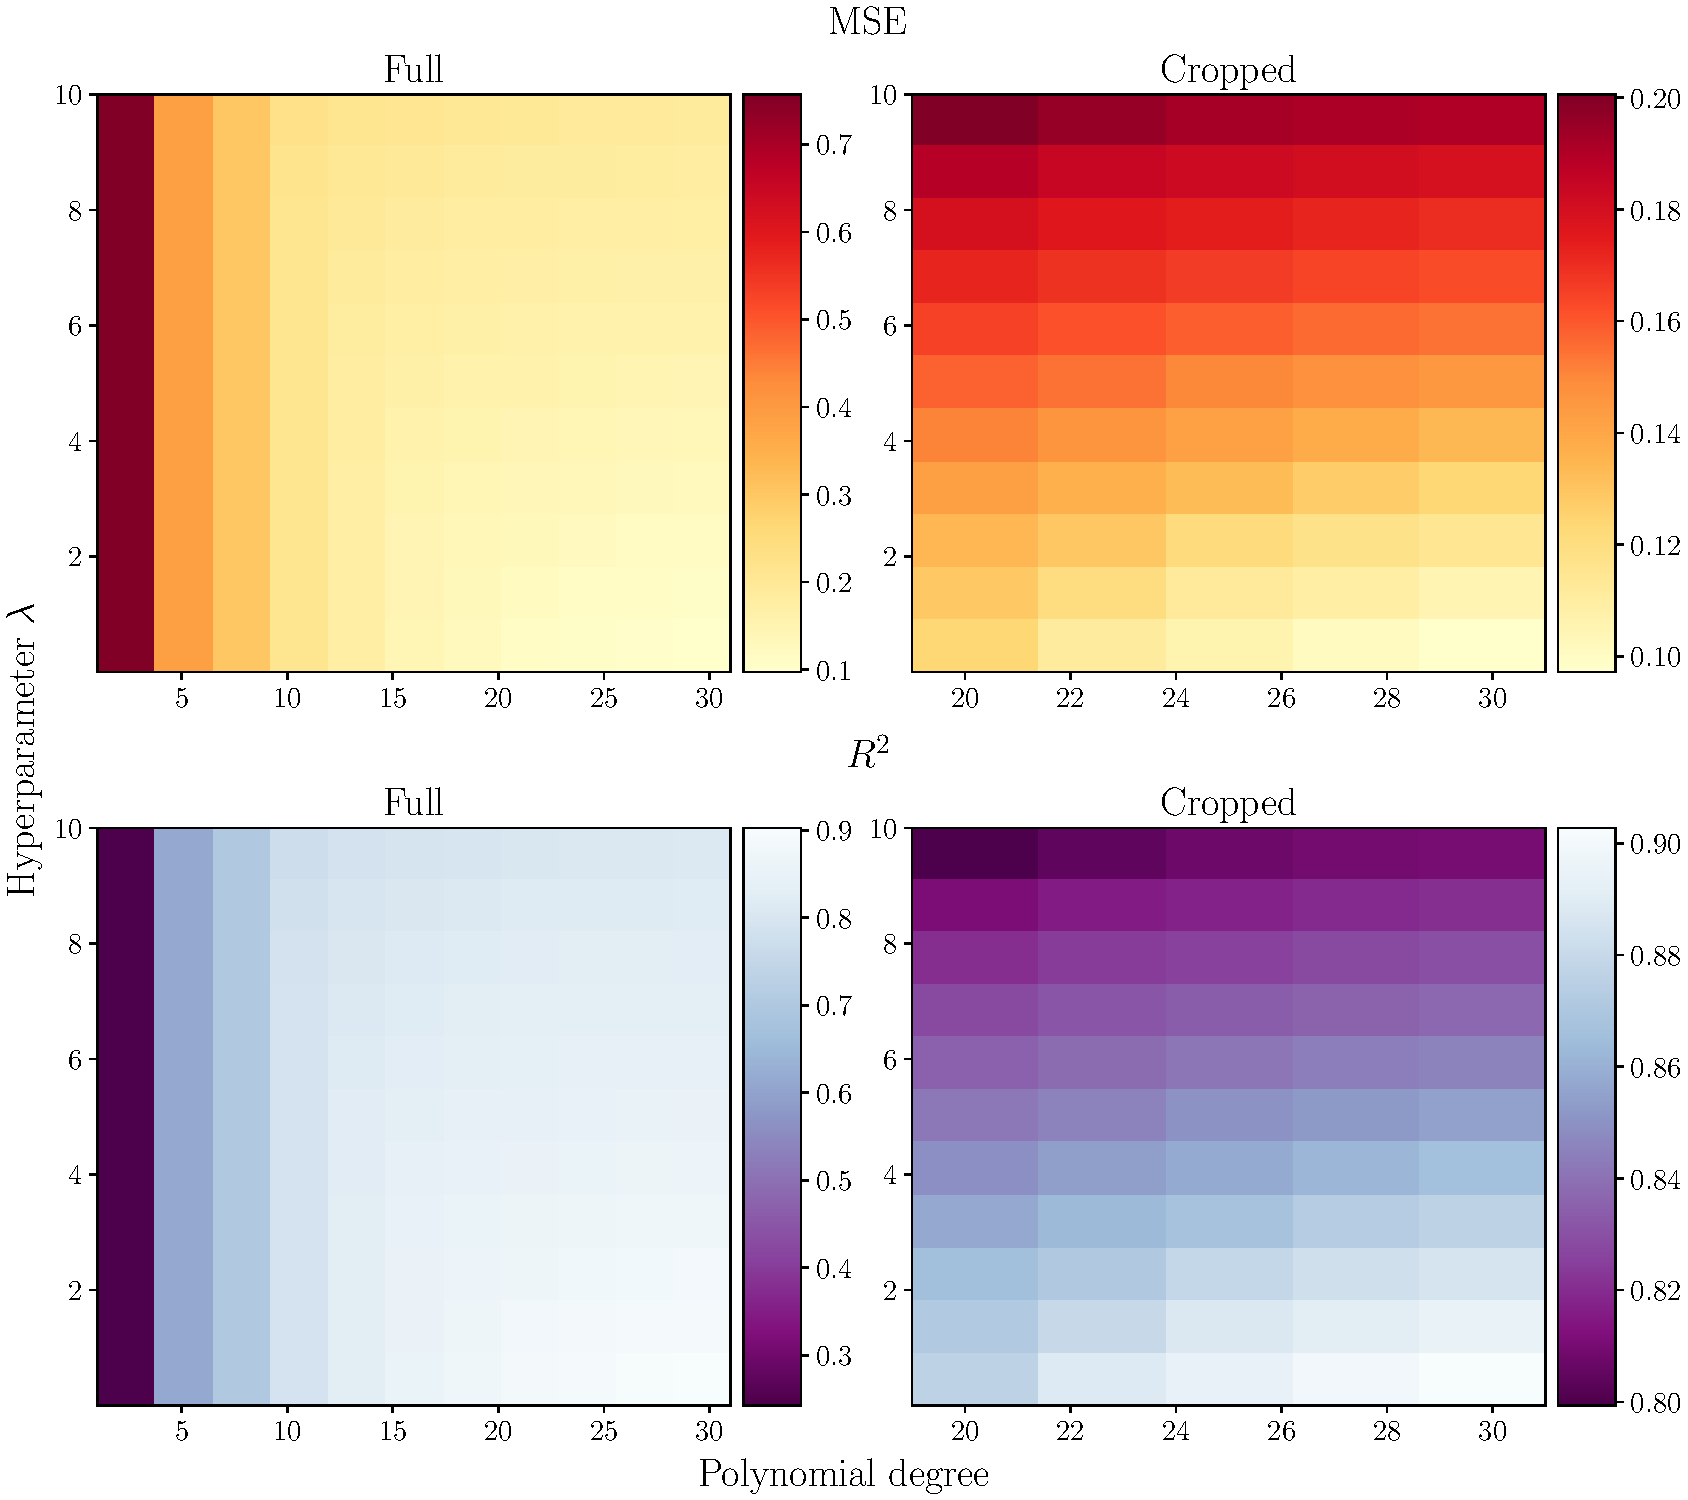
\includegraphics[trim = 0 0.75cm 0 0,clip,width=0.7\textwidth,keepaspectratio]{../figs/g_MSE_R2_Ridge.pdf}
  \centering
  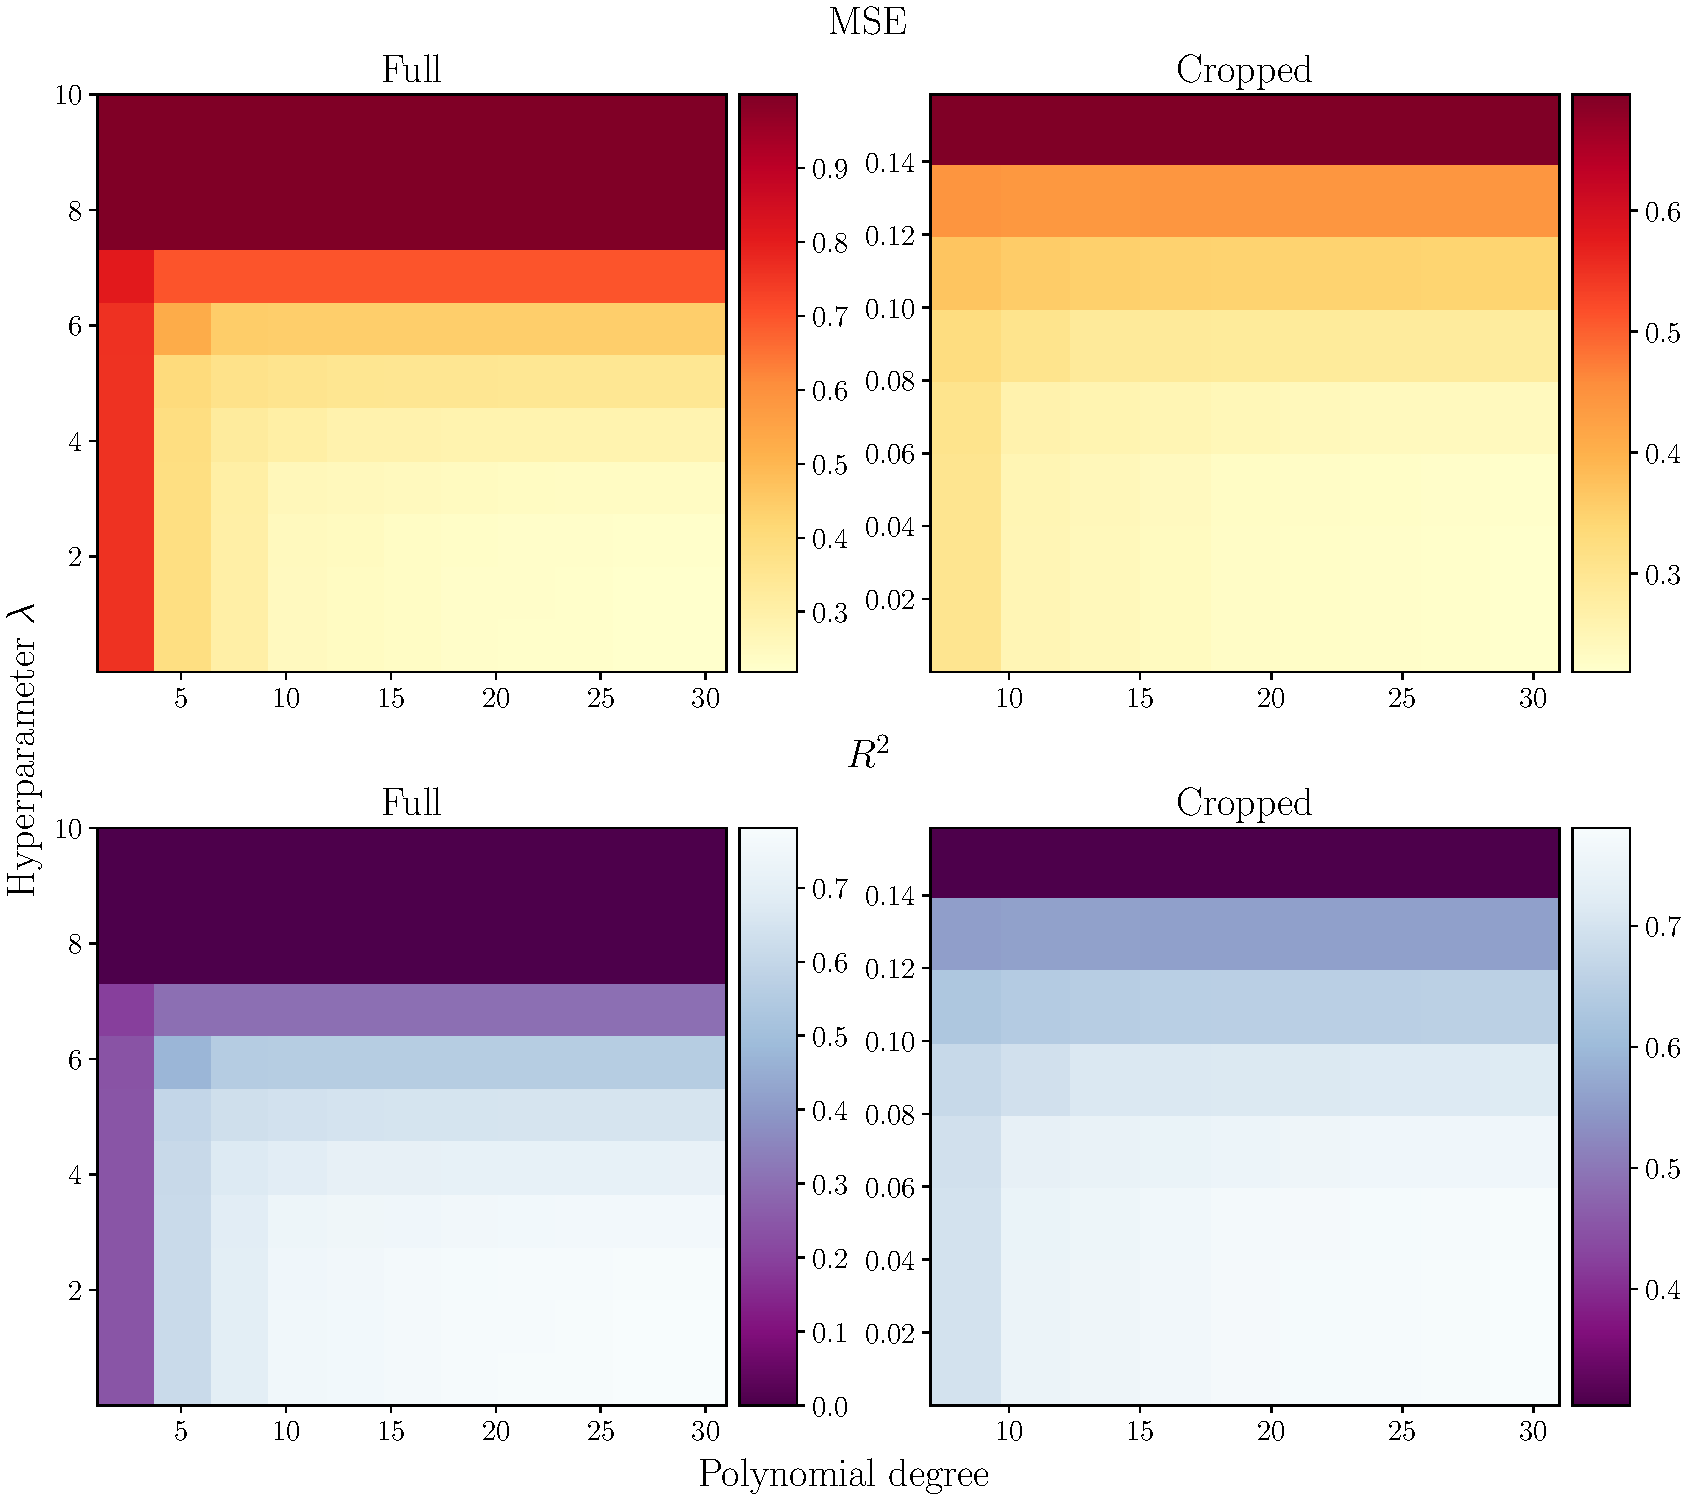
\includegraphics[width=0.7\textwidth]{../figs/g_MSE_R2_Lasso.pdf}
  \caption{MSE (upper rows) and $R^2$ (lower rows) for Ridge (top section) and Lasso (bottom section) regression evaluated on the cosmological test set. The scores vary with polynomial degree horizontally and hyperparameter $\lambda$ vertically. In the right columns we have cropped away degrees smaller than 19, as well as the 3 largest $\lambda$'s only for Lasso, purely for visualization purposes.}\label{appfig:g MSE R2}
  \vspace*{-5pt}
\end{figure*}


\begin{figure*}
  \vspace*{-5pt}
  \centering %Centers the figure
  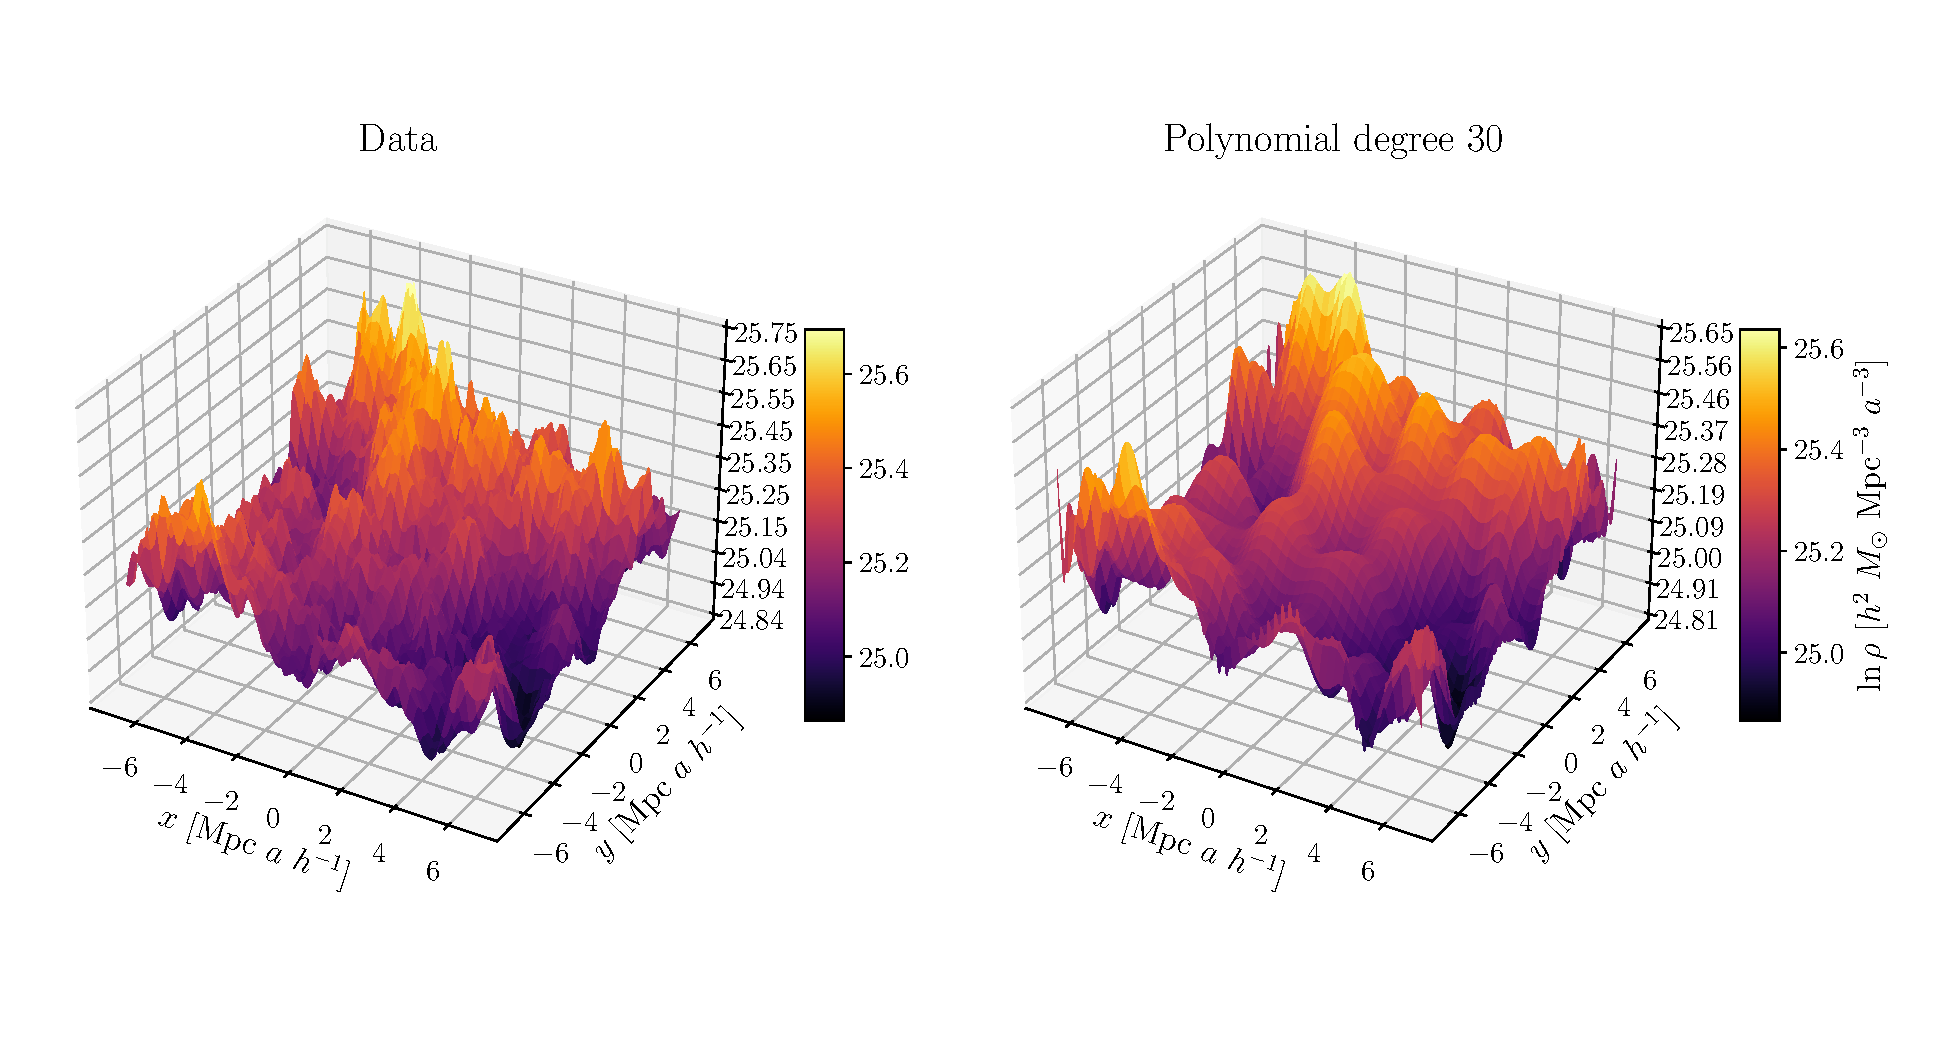
\includegraphics[trim = 0 2cm 0 0,clip,width=\textwidth,keepaspectratio]{../figs/density_surf.pdf}
  \caption{Surface plots of the cosmological simulation data (left) and the OLS fit for polynomial degree 30 (right).}\label{appfig:density surf}
  \vspace*{-5pt}
\end{figure*}


\begin{figure*}
  \vspace*{-5pt}
  \centering %Centers the figure
  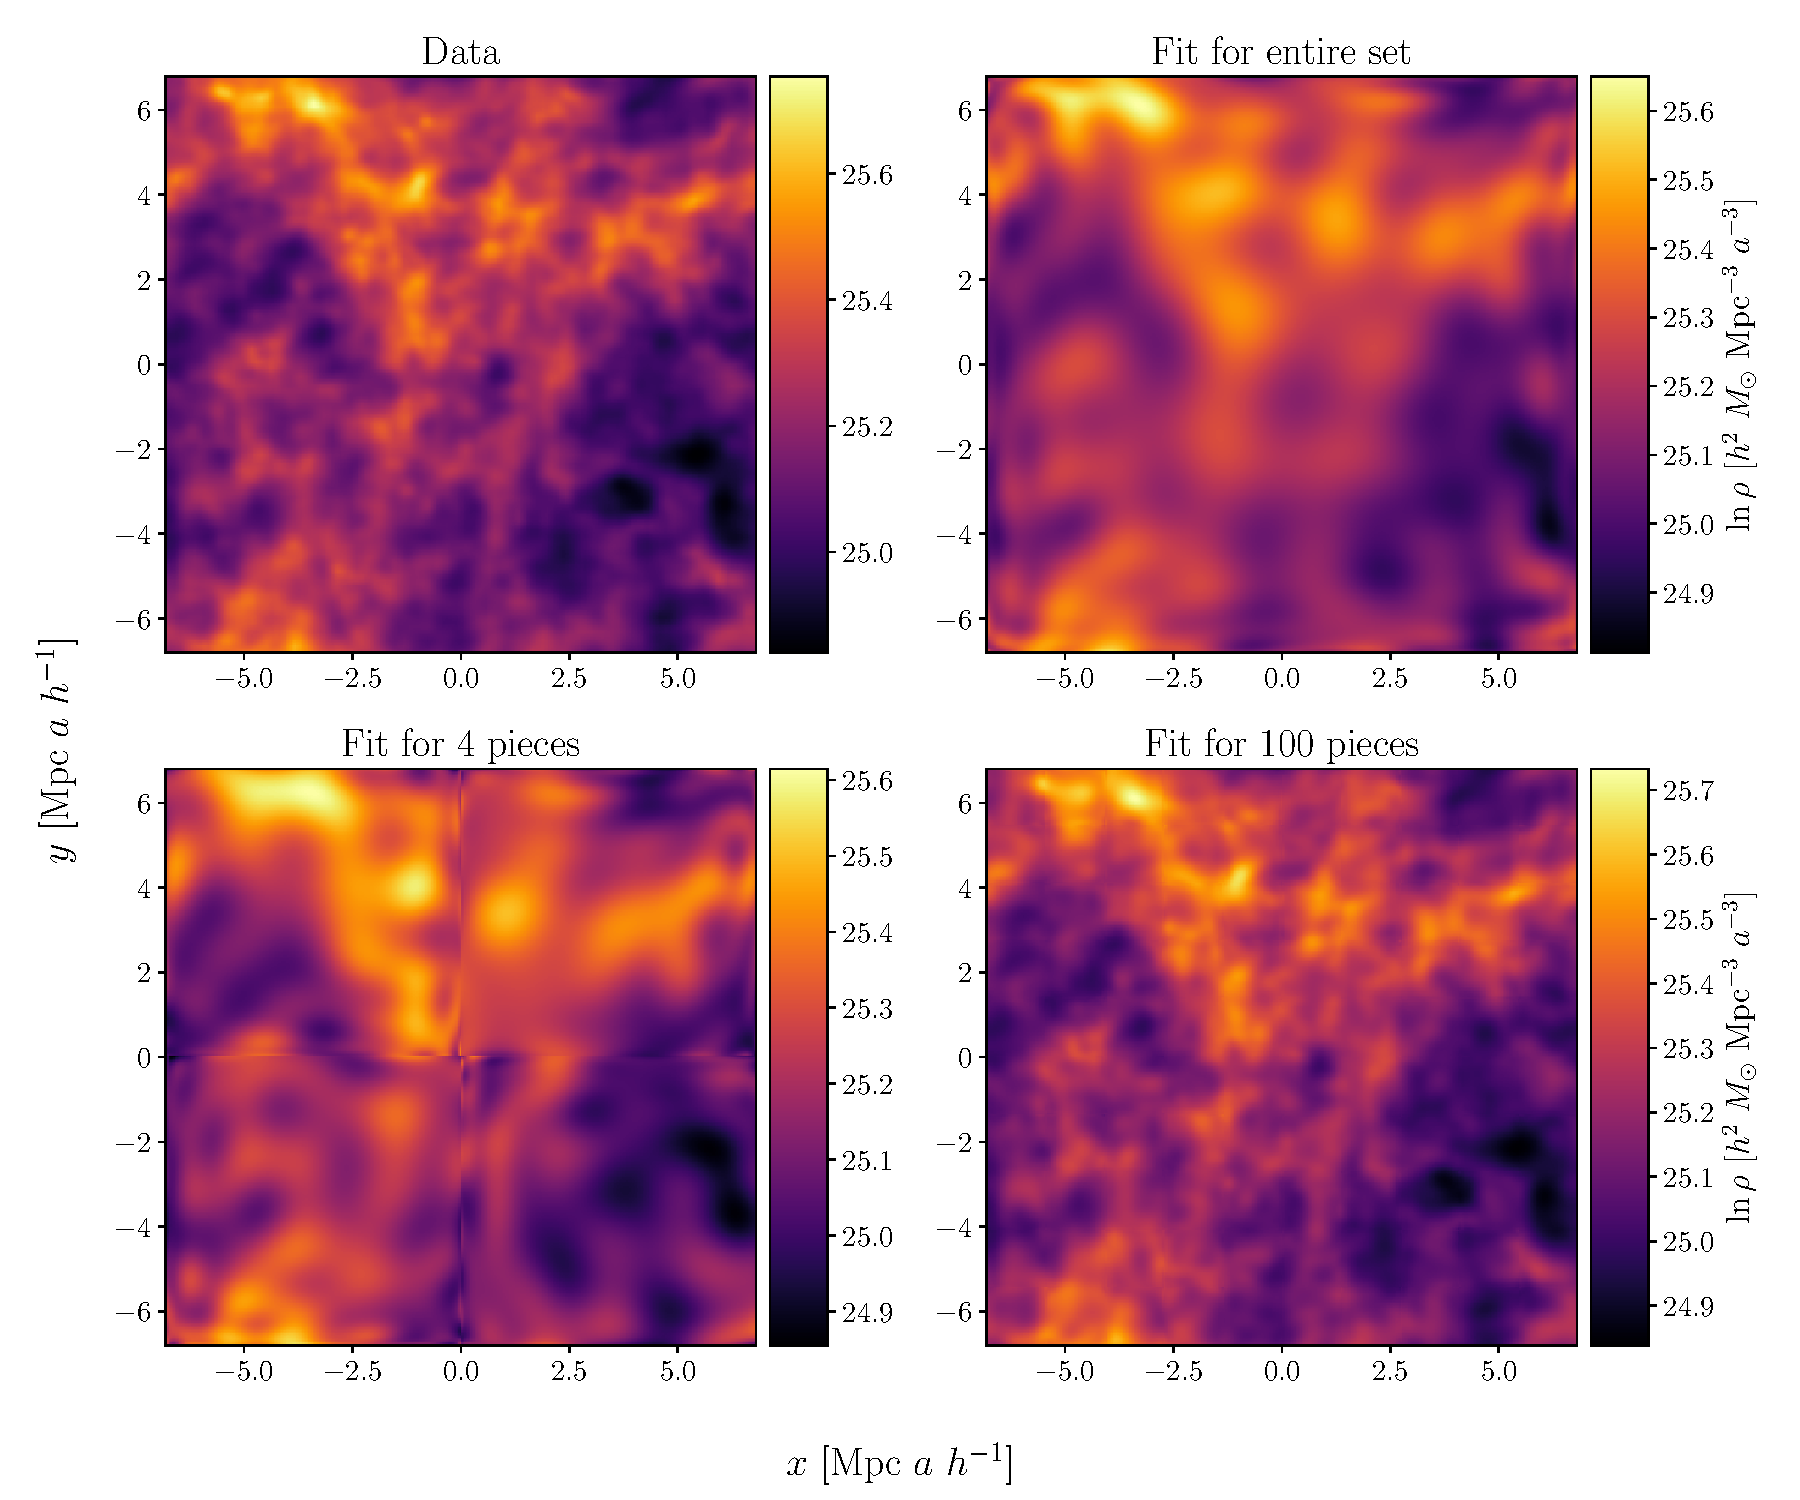
\includegraphics[width=0.8\textwidth]{../figs/density_pieces.pdf}
  \caption{Contour plots of the cosmological simulation data (upper left) and the OLS fits for the entire data (upper right), 4 separate pieces stitched back together (lower left) and 100 separate pieces stitched back together (lower right). We have used a polynomial degree of 30 for all fits.}\label{appfig:density pieces}
  \vspace*{-5pt}
\end{figure*}

\end{document}

% MAYBE REMOVE

% LINK WITH SPECIFIC NAME
% \href{https://raw.github.uio.no/oskarei/CompFys-Project5/main/data/gif/triple_slit_200_81_anim.gif?token=GHSAT0AAAAAAAAAIZKJAEIVBDMTTIDARGUYZMAXTHA}{triple-slit}

% MATHMODE IN HEADLINE
% \subsubsection{\texorpdfstring{$\text{Re}(u_{i,j}^n)$ and $\text{Im}(u_{i,j}^n)$}{Lg}}


% FIGURE COVERING BOTH COLUMNS
% \begin{figure*}
%   \vspace*{-5pt}
%   \centering %Centers the figure
%   \includegraphics[width=\textwidth]{../data/fig/triple_slit.pdf}
%   \caption{The square root of the probabilities at each point in the box $\sqrt{p_{i,j}^n}$ at the beginning (top left), middle (top center) and end (top right) of the triple-slit simulation with adjusted initialization and potential position. The plot at the bottom shows the normalized probability values $p(y\:|\:x=0.9;\;t=0.0025)$ along the detection screen at $x = 0.9$ at the end of the simulation.}\label{fig:TripleSlit}
%   \vspace*{-5pt}
% \end{figure*}

% FIGURE IN SINGLE COLUMN
% \begin{figure}[h!]
%   %\vspace*{-5pt}
%   \centering %Centers the figure
%   \includegraphics[width=0.9\columnwidth]{../data/fig/triple_sketch.png}
%   \caption{Illustration showing how the triple-slit interference pattern changes with distance from the slits. Gathered from Physics StackExchange \cite{TripleSketch}.}\label{fig:TripleSketch}
%   \vspace*{-10pt}
% \end{figure}


% TABLE COVERING BOTH COLUMNS
% \begin{center}
%   \vspace{-10pt}
%   \renewcommand{\arraystretch}{1.5}
%   \begin{table*}
%   %\centering
%   \begin{tabular}{| C{3.5cm} | C{2.2cm} | C{2.2cm} |  C{2.2cm} |  C{2.2cm} |  C{2.2cm} |  C{2.2cm} |}
%   \hline
%   \hspace{1pt} & \textbf{Model \hyperref[fig:potential model A]{A}} & \textbf{Model \hyperref[fig:potential model B]{B}} & \textbf{Model \hyperref[fig:potential model C]{C}} & \textbf{Model \hyperref[fig:potential model D]{D}} & \textbf{Model \hyperref[fig:potential model E]{E}} & \textbf{Model \hyperref[fig:potential model F]{F}} \\
%   \hline
%   \boldmath$m_0/M_{\astrosun}$ & $0.95$ & $0.95$ & $1.00$ & $1.00$ & $1.00$ & $1.05$ \\
%   \hline
%   \boldmath$r_0/R_{\astrosun}$ & $1.00$ & $1.25$ & $1.00$ & $1.00$ & $1.00$ & $1.50$ \\
%   \hline
%   \boldmath$L_0/L_{\astrosun}$ & $1.25$ & $1.00$ & $1.25$ & $1.50$ & $1.50$ & $1.00$ \\
%   \hline
%   \boldmath$\rho_0/\overline{\rho}_{\astrosun}$ & $1.00\times10^{-5}$ & $1.00\times10^{-5}$ & $7.50\times10^{-6}$ & $1.00\times10^{-5}$ & $2.50\times10^{-5}$ & $1.25\times10^{-5}$ \\
%   \hline
%   \textbf{Reach of }\boldmath{$m/m_0$} & $3.02\:\%$ & $4.24\:\%$ & $1.18\:\%$ & $2.66\:\%$ & $4.40\:\%$ & $3.79\:\%$ \\
%   \hline
%   \textbf{Reach of }\boldmath{$r/r_0$} & $0.73\:\%$ & $0.34\:\%$ & $0.06\:\%$ & $0.39\:\%$ & $0.51\:\%$ & $0.19\:\%$ \\
%   \hline
%   \textbf{Reach of }\boldmath{$L/L_0$} & $0.03\:\%$ & $0.14\:\%$ & $0.08\:\%$ & $0.04\:\%$ & $0.11\:\%$ & $0.21\:\%$ \\
%   \hline
%   \textbf{Size of core} & $0.24\times r_0$ & $0.19\times r_0$ & $0.26\times r_0$ & $0.25\times r_0$  & $0.24\times r_0$  & $0.15\times r_0$ \\
%   \hline
%   \textbf{Width of main zone} & $0.21\times r_0$ & $0.24\times r_0$ & $0.17\times r_0$ & $0.21\times r_0$ & $0.30\times r_0$ & $0.28\times r_0$ \\
%   \hline
%   \boldmath$F_\textbf{small}/F_\textbf{main}$ & No zone & No zone & $8.39\:\%$ & No zone & No zone & No zone \\
%   \hline
%   \end{tabular}
%   \cprotect\caption{The first four rows contain the initial mass, radius, luminosity and mass density of the six models, respectively. The initial temperature was $T_0 = 5770\:\text{K}$ for all six models, and the initial pressure was decided by the initial mass density through the equation of state. The next three rows show how far $m$, $r$ and $L$ reached before the integration was stopped, respectively. The size of the core and of the main convection zone near the surface, both given in units of $r_0$, are listed in the two next rows. In the last row I have listed the ratios between the convective flux from an eventual second, smaller convection zone and the convective flux from the respective main convection zone. If it says ``No zone'', the model does not have any more convection zones.}\label{tab:models}
%   \end{table*}
%   \renewcommand{\arraystretch}{1}
%   \vspace{-20pt}
% \end{center}

% STANDARD TABLE IN SINGLE COLUMN
% \begin{center}
%   \renewcommand{\arraystretch}{1.5}
%   \begin{table}[h!]
%   \centering
%   \begin{tabular}{| C{2.2cm} | C{1.4cm} | C{1.4cm} | C{1.4cm} | C{1.4cm} |}
%   \hline
%   \textbf{No. of cycles} & \boldmath$\left<ϵ\right>$ \boldmath$[J]$ & \boldmath$\left<|m|\right>$ & \boldmath$C_V$ \boldmath$[k_\text{B}]$ & \boldmath$\chi$ \boldmath$[J^{-1}]$ \\
%   \hline
%   10 & $-1.8000$ & 0.9375 & 1.4400 & 0.1594 \\
%   \hline
%   20 & $-1.9000$ & 0.9688 & 0.7600 & 0.0836 \\
%   \hline
%   50 & $-1.9600$ & 0.9875 & 0.3136 & 0.0344 \\
%   \hline
%   100 & $-1.9800$ & 0.9938 & 0.1584 & 0.0173 \\
%   \hline
%   200 & $-1.9775$ & 0.9931 & 0.1780 & 0.0186 \\
%   \hline
%   500 & $-1.9880$ & 0.9962 & 0.0954 & 0.0104 \\
%   \hline
%   1000 & $-1.9940$ & 0.9981 & 0.0479 & 0.0052 \\
%   \hline
%   5000 & $-1.9960$ & 0.9988 & 0.0319 & 0.0033 \\
%   \hline
%   10000 & $-1.9974$ & 0.9992 & 0.0204 & 0.0022 \\
%   \hline
%   100000 & $-1.9975$ & 0.9992 & 0.0197 & 0.0022 \\
%   \hline
%   1000000 & $-1.9973$ & 0.9992 & 0.0215 & 0.0023 \\
%   \hline
%   \textbf{Analytical} & $-1.9960$ & 0.9987 & 0.0321 & 0.0040 \\
%   \hline
%   \end{tabular}
%   \cprotect\caption{Numerical estimates of $\left<\epsilon\right>$, $\left<|m|\right>$, $C_V$ and $\chi$ for $T = 1.0\:J/k_\text{B}$ after increasing numbers of Monte Carlo cycles are performed. The last row contains the analytical values.}\label{tab:2x2 results}
%   \end{table}
%   \renewcommand{\arraystretch}{1}
% \end{center}

% TABLE WITH MULTIROW
% \begin{center}
%   \renewcommand{\arraystretch}{1.5}
%   \begin{table}[h!]
%   \centering
%   \begin{tabular}{| C{2.4cm} | C{1.5cm} | C{1.1cm} | C{2.0cm} |}
%   \hline
%   \textbf{No. of} \boldmath$s = +1$ & \boldmath$E(\mathbf{s})$ \boldmath$[J]$ & \boldmath$M(\mathbf{s})$ & \textbf{Degeneracy} \\
%   \hline
%   0 & $-8$ & $-4$ & None \\
%   \hline
%   1 & \hspace{7pt}$0$ & $-2$ & $4$ \\
%   \hline
%   \multirow{2}{*}{2} & \hspace{7pt}$8$ & \multirow{2}{*}{\hspace{7pt}$0$} & $2$ \\
%   \cline{2-2}\cline{4-4}
%   & \hspace{7pt}$0$ & & $4$ \\
%   \hline
%   3 & \hspace{7pt}$0$ & \hspace{7pt}$2$ & $4$ \\
%   \hline
%   4 & $-8$ & \hspace{7pt}$4$ & None \\
%   \hline
%   \end{tabular}
%   \cprotect\caption{Total energy $E(\mathbf{s})$ and magnetisation $M(\mathbf{s})$ for a \texorpdfstring{$2\times2$}{Lg} lattice with $0$, $1$, $2$, $3$ and $4$ spins $s = +1$. Because we use periodic boundary conditions, the total energy can either be 0$\:J$ or 8$\:J$ when we have two spins $s = +1$ and two spins $s = -1$, depending on if the equal spins are neighbours or not. The last column contains the degeneracy level for the different combinations of number of spins $s = +1$ and total energy.}\label{tab:2x2 lattice}
%   \end{table}
%   \renewcommand{\arraystretch}{1}
% \end{center}


% ALGORITHM
% \begin{figure}
%   % NOTE: We only need \begin{figure} ... \end{figure} here because of a compatability issue between the 'revtex4-1' document class and the 'algorithm' environment.
%       \begin{algorithm}[H]
%       \caption{The Metropolis Algorithm}
%       \label{algo:Euler}
%           \begin{algorithmic}
%               \Procedure{Monte Carlo cycle}{$\mathbf{s}, L, β$}
%               \For{$i = 0, 1, \ldots, L-1$}
%               \For{$j = 0, 1, \ldots, L-1$}
%               \State $\triangleright$ Compute energy difference due to flipping $s_{ij}$
%               \State $\Delta E ← \Delta E_\text{function}(\mathbf{s}, i, j)$
%               \State
%               \State $\triangleright$ Flip if energy difference is negative or zero
%               \If{$\Delta E \leq 0$}
%                   \State $s_{ij} = -s_{ij}$ \Comment{Flip spin}
%                   \State
%               \Else \Comment{Energy difference is positive}
%                   \State $w = e^{-β\Delta E}$ \Comment{Probability of flipping spin}
%                   \State $\triangleright$ Generate random number $r ∈ [0,1]$
%                   \State $\triangleright$ Flip spin if $r≤ w$
%                   \If{$r≤ w$}
%                       \State $s_{ij} = -s_{ij}$ \Comment{Flip spin}
%                   \EndIf
%               \EndIf
%               \State 
%               \State $\triangleright$ Calculate $E$, $E^2$, $|M|$ and $M^2$ for $\mathbf{s}$
%               \State $E$, $E^2 = E_\text{function}(\mathbf{s})$
%               \State $|M|$, $M^2 = M_\text{function}(\mathbf{s})$
%               \State $\triangleright$ Update expectation values accordingly
%               \EndFor
%               \EndFor
%               \EndProcedure
%           \end{algorithmic}
%       \end{algorithm}
%   \end{figure}